\documentclass[type=doctor]{thuthesis}
% 选项:
%   type=[bachelor|master|doctor|postdoctor], % 必选
%   secret,                                   % 可选
%   pifootnote,                               % 可选(建议打开)
%   openany|openright,                        % 可选,基本不用
%   arial,                                    % 可选,基本不用
%   arialtoc,                                 % 可选,基本不用
%   arialtitle                                % 可选,基本不用

% 所有其它可能用到的包都统一放到这里了,可以根据自己的实际添加或者删除。
\usepackage{thuthesis}
\usepackage{tikz}
\usetikzlibrary{arrows.meta} 
\usepackage{tensor}
\usepackage{xspace}
\usepackage{alltt}
%\usepackage{pdflscape}
\usepackage{lscape} 
\usepackage[boxed]{algorithm2e}
\usepackage{mathpartir}
\usepackage{amssymb}
\usepackage{wasysym}
\usepackage{marvosym}
\usepackage{pifont}



%\usepackage{amsmath,amssymb,latexsym} 
%\usepackage{stmaryrd}

% 定义所有的图片文件在 figures 子目录下
\graphicspath{{figures/}}

% 可以在这里修改配置文件中的定义。导言区可以使用中文。
% \def\myname{薛瑞尼}

%%% calligraphic letters
\newcommand{\cA}{\mathcal{A}}
\newcommand{\cB}{\mathcal{B}}
\newcommand{\cC}{\mathcal{C}}
\newcommand{\cD}{\mathcal{D}}
\newcommand{\cE}{\mathcal{E}}
\newcommand{\cF}{\mathcal{F}}
\newcommand{\cG}{\mathcal{G}}
\newcommand{\cH}{\mathcal{H}}
\newcommand{\cI}{\mathcal{I}}
\newcommand{\cL}{\mathcal{L}}
\newcommand{\cM}{\mathcal{M}}
\newcommand{\cN}{\mathcal{N}}
\newcommand{\cO}{\mathcal{O}}
\newcommand{\cP}{\mathcal{P}}
\newcommand{\cR}{\mathcal{R}}
\newcommand{\cS}{\mathcal{S}}
\newcommand{\cT}{\mathcal{T}}
\newcommand{\cV}{\mathcal{V}}
\newcommand{\cX}{\mathcal{X}}
\newcommand{\cY}{\mathcal{Y}}

%%% brackets
\newcommand{\lb}{\langle}
\newcommand{\rb}{\rangle}

%%% arrows
\newcommand{\la}{\leftarrow}
\newcommand{\ra}{\rightarrow}
\newcommand{\da}{\downarrow}
\newcommand{\ua}{\uparrow}
\newcommand{\dive}{\uparrow\vspace{0.5mm}\uparrow}
\newcommand{\lra}{\leftrightarrow}
\newcommand{\lh}{\leftharpoons}
\newcommand{\rh}{\rightharpoons}
\newcommand{\rlh}{\rightleftharpoons}
\newcommand{\Lla}{\longleftarrow}
\newcommand{\Lra}{\longrightarrow}
\newcommand{\Llra}{\longleftrightarrow}
\newcommand{\Dla}{\Leftarrow}
\newcommand{\Dra}{\Rightarrow}
\newcommand{\Dda}{\Downarrow}
\newcommand{\Dua}{\Uparrow}
\newcommand{\Dlra}{\Leftrightarrow}
\newcommand{\Nla}{\not\rightarrow}
\newcommand{\Nra}{\not\leftarrow}
\newcommand{\raa}{\ra_{aliens}}
\newcommand{\rac}{\ra_{cap}}
\newcommand{\raA}{\ra_{A}}
\newcommand{\raC}{\ra_{C}}
%\newcommand{\nf}[1]{#1\!\!\downarrow}

\newcommand{\Var}[1]{\mathcal{V}ar({#1})}
\newcommand{\FVar}[1]{\mathcal{FV}ar({#1})}
\newcommand{\Pos}[1]{\mathcal{P}os({#1})}
\newcommand{\FPos}[1]{\mathcal{FP}os({#1})}
\newcommand{\VPos}[1]{\mathcal{VP}os({#1})}
\newcommand{\rootp}{\mbox {\footnotesize $\Lambda$}}
\newcommand{\Dom}[1]{\mathcal{D}om({#1})}
\newcommand{\TFX}{\cT(\cF,\cX)}
\newcommand{\GTF}{\cT(\cF)}
\newcommand{\Ran}[1]{{\cV\cR}an({#1})}

\renewcommand{\emptyset}{\varnothing}

%%% macros specifiques
\newcommand{\nat}{\mbox{$I\!\!N$}}
\newcommand{\vect}[1]{\overline{#1}}
%\newcommand{\interp}[1]{\mbox{$[\!\mid \!\! #1 \!\! \mid\!]$}}
\newcommand{\interp}[1]{\llbracket #1 \rrbracket}
%\newcommand{\Ft}{\mbox{$F_{\textit{T}}$}\xspace}
%\newcommand{\Fnt}{\mbox{$F_{\textit{NT}}$}\xspace}




%%% orders
% for labels
\newcommand{\ordl}{\gtordl}
\newcommand{\gtordl}{\rhd}
\newcommand{\geordl}{\unrhd}
\newcommand{\ltordl}{\lhd}
\newcommand{\leordl}{\unlhd}
% for positions
\newcommand{\gtordp}{>_{\cP}}
\newcommand{\geordp}{\ge_{\cP}}
\newcommand{\ltordp}{<_{\cP}}
\newcommand{\leordp}{\le_{\cP}}
\newcommand{\ordp}{\gtordp}
% for subsumption
\newcommand{\gtsubs}{\gtrdot}   %{{\scriptsize \bullet}{\hspace{-0.75mm}>}}
\newcommand{\gesubs}{\mathrel{\stackrel{\scriptscriptstyle\bullet}{}{\!\!\!\!\geq}}}
%\newcommand{\gesubs}{\mathrel{\cdot\!\!\!\geq}}
% for conversions
\newcommand{\po}{\mathrel{\succ\!\!\succ}}
\newcommand{\poeq}{\mathrel{\succeq\!\!\succeq}}
% others
\newcommand{\ordo}{\succ}
\newcommand{\rpo}{\succ_H}
\newcommand{\gerpo}{\succeq_H}
\newcommand{\rpomul}{\,(\rpo)_{mul}\,}
\newcommand{\gerpomul}{\,(\gerpo)_{mul}\,}



\newcommand{\cp}[1]{\cC\cP(#1)}
\newcommand{\pcp}[1]{\cP\cC\cP(#1)}
\newcommand{\hcp}[1]{\cH\cC\cP(#1)}

\newcommand{\lmm}[1]{\vect{#1}}
\newcommand{\mm}[1]{mm({#1})}

%\newcommand{\lll}[1]{ll(#1)}
\newcommand{\rll}[1]{rl(#1)}
\newcommand{\ml}[1]{\cL(#1)}

\newcommand{\fp}[1]{\mbox{\textsc{F}$_{\textsc p}$($#1$)}}
\newcommand{\vL}[1]{{\textsc{vl}}(#1)}
\newcommand{\vS}[1]{{\textsc{vs}}(#1)}
\newcommand{\vs}[1]{{\textsc{sh}}(#1)}
\newcommand{\hp}[1]{\cH p(#1)}
\newcommand{\hit}[1]{\cH t(#1)}
\newcommand{\IC}[1]{\cI\cC(#1)}
\newcommand{\lp}[1]{#1_{\mathit{peak}}}
\newcommand{\lc}[1]{#1_{\mathit{conv}}}
\newcommand{\lcl}[1]{#1_{\mathit{cliff}}} %added by jiaxiang
\newcommand{\lcp}[1]{#1_{\mathit{convp}}} %added by jiaxiang
\newcommand{\lcc}[1]{#1_{\mathit{convc}}} %added by jiaxiang

\newcommand{\equivp}[2]{~\equiv^{#1}_{#2}~}
\newcommand{\repl}{{\cR}epl}

%\newcommand{\RT}{R_{{\textsc{t}\xspace}}}
%\newcommand{\RNT}{R_{{\textsc{nt}\xspace}}}

%labelled rewriting
%Optional Args 1: position, 2:label, 3:rule or rule set, 4:substitution.
\newcommand{\lablrps}[4]{\mathop{\longrightarrow}^{#1,#2}_{#3,#4}}
\newcommand{\dlablrps}[4]{\displaystyle \lablrps{#1}{#2}{#3}{#4}}
\newcommand{\lablrpps}[4]{\mathop{\Longrightarrow}^{#1,#2}_{#3,#4}}
\newcommand{\dlablrpps}[4]{\displaystyle \lablrpps{#1}{#2}{#3}{#4}}

% rewriting
%% \newcommand{\lrps}[2]{{\mathop{\longrightarrow}^{#1}_{#2}}}
\newcommand{\lrps}[2]{\mathrel{\ra^{#1}_{#2}}} % new def
\newcommand{\llrps}[2]{~\lrps{#1}{#2}~}
\newcommand{\dlrps}[2]{\displaystyle \lrps{#1}{#2}}
\newcommand{\dllrps}[2]{\displaystyle \llrps{#1}{#2}}
%% \newcommand{\rlps}[2]{{^{~#1}_{#2}\!\!\mathop{\longleftarrow}}}
%%\newcommand{\rlps}[2]{\mathrel{\prescript{#1\!\!\;}{#2}{\!\!\;\la}}} % new def
%% \newcommand{\rlps}[2]{\mathrel{\myprescript{#1\!\!\;}{#2}{\!\!\;\la}}} % new def
\newcommand{\rlps}[2]{\mathrel{\!\tensor*[^{#1\!\!\;}_{#2}]{\!\!\;\la}{}}} % new def
\newcommand{\lrlps}[2]{~\rlps{#1}{#2}~}
\newcommand{\rlpsbis}[2]{\mathop{\longleftarrow}^{\,#1}_{#2}}
\newcommand{\drlps}[2]{{\displaystyle \rlpsbis{#1}{#2}}}
\newcommand{\dlrlps}[2]{~\drlps{#1}{#2}~}
\newcommand{\Lrps}[2]{\mathrel{\Rightarrow^{#1}_{#2}}} % new def
\newcommand{\Rlps}[2]{\mathrel{\prescript{#1\!\!\;}{#2}{\!\!\;\Leftarrow}}} % new def

%\newcommand{\DLrps}[2]{\mathop{\Longrightarrow}^{#1}_{#2}}
%\newcommand{\TLrps}[2]{\mathop{\Longrightarrow\!\!\succ}^{#1}_{#2}}

% parallel rewriting
%\newcommand{\llrpps}[2]{~\Lrps{#1}{#2}~}
%\newcommand{\Rlps}[2]{\mathop{\Longleftarrow}^{#1}_{#2}}
%\newcommand{\lrlpps}[2]{~\Rlps{#1}{#2~}}

%% symmetric closures
\newcommand{\eqps}[2]{\mathrel{\lra^{#1}_{#2}}} % new def
\makeatletter
\newcommand{\shorteq}{%
  \settowidth{\@tempdima}{-}% Width of hyphen
  \resizebox{\@tempdima}{\height}{=}%
}
\makeatother
%% \newcommand{\eqpseq}[2]{{\mathop{\:\;{\tiny =}\:\!\!\!\!\!\!\!\!\!\!\!\longleftrightarrow}^{#1}_{#2}}}
\newcommand{\eqpseq}[2]{\mathrel{\mathrel{\lra\!\!\!\!\!\!\!\:\shorteq\,\,}^{#1}_{#2}}} % new def 
\newcommand{\deqpseq}[2]{\displaystyle \eqpseq{#1}{#2}}

%% \newcommand{\conv}[2]
%%            {{\mathop{\la\!\!\!\!\!\longleftrightarrow\!\!\!\!\!\ra}^{#1}_{#2}}}
\newcommand{\conv}[2]{\mathrel{\la\!\!\!\!\!\lra\!\!\!\!\!\ra^{#1}_{#2}}} % new def
\newcommand{\lconv}[2]{~\conv{#1}{#2}~}
\newcommand{\dconv}[2]{\displaystyle \conv{#1}{#2}}
\newcommand{\dlconv}[2]{~\dconv{#1}{#2}~}
%\newcommand{\conv}[1]{\displaystyle \convv{#1}}


%% reflexive closures
%% \newcommand{\lrpseq}[2]{{\mathop{\longrightarrow\!\!\!\!\!\!\!{\tiny =}}^{#1}_{#2}}}
\newcommand{\lrpseq}[2]{\mathrel{\mathrel{\ra\!\!\!\!\!\!\:\shorteq\,}^{#1}_{#2}}} % new def
\newcommand{\llrpseq}[2]{~\lrpseq{#1}{#2}~}
\newcommand{\dlrpseq}[2]{\displaystyle \lrpseq{#1}{#2}}
\newcommand{\dllrpseq}[2]{\displaystyle \llrpseq{#1}{#2}}
%% \newcommand{\rlpseq}[2]{{~^{~#1}_{#2}\mathop{\!{\tiny =}\!\!\!\!\!\!\!\longleftarrow}}}
\newcommand{\rlpseq}[2]{\mathrel{\prescript{#1\!\!\;}{#2}{\;\!\shorteq\!\!\!\!\!\!\:\la}}} % new def
\newcommand{\lrlpseq}[2]{~\rlpseq{#1}{#2}~}
\newcommand{\rlpseqis}[2]{\mathop{{\tiny =}\!\!\!\!\!\!\!\longleftarrow}^{#1}_{#2}}
\newcommand{\drlpseq}[2]{\,{\displaystyle \rlpseqis{#1}{#2}}}
\newcommand{\dlrlpseq}[2]{~\drlpseq{#1}{#2}~}
%\newcommand{\lrppseq}[1]{\mathop{\Longrightarrow\!\!\!\!\!\!\!{\tiny =}}^{#1}}
%\newcommand{\rlppseq}[1]{\mathop{{\tiny =}\!\!\!\!\!\!\!\Longleftarrow}^{#1}}


%% derivations
%% \newcommand{\lrder}[2]{{\mathop{\longrightarrow\!\!\!\!\!\ra}^{#1}_{#2}}}
\newcommand{\lrder}[2]{\mathrel{\ra\!\!\!\!\!\ra^{#1}_{#2}}} % new def
\newcommand{\llrder}[2]{~\lrder{#1}{#2}~}
\newcommand{\dlrder}[2]{\displaystyle \lrder{#1}{#2}}
\newcommand{\dllrder}[2]{~\dlrder{#1}{#2}~}
%% \newcommand{\rlder}[2]{{~^{~#1}_{#2}\!\!\mathop{\la\!\!\!\!\!\longleftarrow}}}
\newcommand{\rlder}[2]{\mathrel{\prescript{#1\!\!\;}{#2}{\!\!\;\la\!\!\!\!\!\la}}} % new def
\newcommand{\lrlder}[2]{~\rlder{#1}{#2}~}
\newcommand{\rlderis}[2]{\mathop{\la\!\!\!\!\!\longleftarrow}^{~#1}_{#2}}
\newcommand{\drlder}[2]{{\displaystyle \rlderis{#1}{#2}}}
\newcommand{\dlrlder}[2]{~\drlder{#1}{#2}~}

\newcommand{\ordt}{\mbox{$\succ\!\!\succ$}}
\newcommand{\geordt}{\mbox{$\succeq\!\!\succeq$}}

%% others
\newcommand{\LrpsD}{\Longrightarrow_\cD}
\newcommand{\RlpsD}{_\cD\!\!\Longleftarrow}



\newcommand{\hide}[1]{\ignorespaces}
\newcommand{\todo}[1]{\textbf{TODO: } #1}
\renewcommand{\algorithmcfname}{算法}

\newcommand{\zero}{\operatorname{\mathsf{zero}}}
\newcommand{\s}{\operatorname{\mathsf{s}}}
\newcommand{\add}{\operatorname{\mathsf{add}}}
\newcommand{\lessthan}{\operatorname{\mathsf{lessthan}}}
\newcommand{\true}{\operatorname{\mathsf{true}}}
\newcommand{\false}{\operatorname{\mathsf{false}}}
\newcommand{\mynot}{\operatorname{\mathsf{not}}}
\newcommand{\farmer}{\operatorname{\mathsf{farmer}}}
\newcommand{\wolf}{\operatorname{\mathsf{wolf}}}
\newcommand{\lamb}{\operatorname{\mathsf{lamb}}}
\newcommand{\grass}{\operatorname{\mathsf{grass}}}
\newcommand{\lhs}{\operatorname{\mathsf{left}}}
\newcommand{\rhs}{\operatorname{\mathsf{right}}}
\newcommand{\change}{\operatorname{\mathsf{change}}}
\newcommand{\comp}{\operatorname{\mathsf{::}}}
\renewcommand{\clock}{\operatorname{\mathsf{clock}}}
\newcommand{\broken}{\operatorname{\mathsf{broken}}}
\newcommand{\myempty}{\operatorname{\mathsf{empty}}}

\newcommand{\defeq}{\ensuremath{\stackrel{\text{\tiny def}}{=}}}
\newcommand{\nf}[2]{{#1}\!\da_{#2}\xspace}
\newcommand{\RE}{\cR_{\cE}}
\newcommand{\SE}{\cS_{\cE}}
\newcommand{\RSE}{\cR_{\cS\cE}}
\newcommand{\VP}{\cV_{\cP}}
\newcommand{\Vsym}{\cV_{sym}}
\newcommand{\pta}{\hookrightarrow}
\newcommand{\ty}{\texttt{ty}}
\newcommand{\transto}{\rightsquigarrow}

\newcommand{\allsup}{\ding{51}}
\newcommand{\halfsup}{\CheckedBox}
\newcommand{\nonsup}{\ding{55}}

\newcommand\TTT{%
 \textsf{T\kern-0.2em\raisebox{-0.3em}T\kern-0.2emT\kern-0.2em\raisebox{-0.3em}2}%
}

\newcommand{\CTerm}{{Ceagle-\textsc{Term}}}

\begin{document}

%%% 封面部分
\frontmatter
\thusetup{
  %******************************
  % 注意:
  %   1. 配置里面不要出现空行
  %   2. 不需要的配置信息可以删除
  %******************************
  %
  %=====
  % 秘级
  %=====
  secretlevel={秘密},
  secretyear={10},
  %
  %=========
  % 中文信息
  %=========
  ctitle={基于重写理论的嵌入式系统建模与验证},
  cdegree={工学博士},
  cdepartment={计算机科学与技术系},
  cmajor={计算机科学与技术},
  cauthor={刘嘉祥},
  csupervisor={顾 明教授},
  cassosupervisor={孙家广教授}, % 副指导老师
  % ccosupervisor={某某某教授}, % 联合指导老师
  % 日期自动使用当前时间,若需指定按如下方式修改:
  % cdate={超新星纪元},
  %
  % 博士后专有部分
  cfirstdiscipline={计算机科学与技术},
  cseconddiscipline={系统结构},
  postdoctordate={2009年7月——2011年7月},
  id={编号}, % 可以留空: id={},
  udc={UDC}, % 可以留空
  catalognumber={分类号}, % 可以留空
  %
  %=========
  % 英文信息
  %=========
  etitle={An Introduction to \LaTeX{} Thesis Template of Tsinghua University v\version},
  % 这块比较复杂,需要分情况讨论:
  % 1. 学术型硕士
  %    edegree:必须为Master of Arts或Master of Science(注意大小写)
  %             “哲学、文学、历史学、法学、教育学、艺术学门类,公共管理学科
  %              填写Master of Arts,其它填写Master of Science”
  %    emajor:“获得一级学科授权的学科填写一级学科名称,其它填写二级学科名称”
  % 2. 专业型硕士
  %    edegree:“填写专业学位英文名称全称”
  %    emajor:“工程硕士填写工程领域,其它专业学位不填写此项”
  % 3. 学术型博士
  %    edegree:Doctor of Philosophy(注意大小写)
  %    emajor:“获得一级学科授权的学科填写一级学科名称,其它填写二级学科名称”
  % 4. 专业型博士
  %    edegree:“填写专业学位英文名称全称”
  %    emajor:不填写此项
  edegree={Doctor of Engineering},
  emajor={Computer Science and Technology},
  eauthor={Liu Jiaxiang},
  esupervisor={Professor Gu Ming},
  eassosupervisor={Professor Sun Jiaguang},
  % 日期自动生成,若需指定按如下方式修改:
  % edate={December, 2005}
  %
  % 关键词用“英文逗号”分割
  ckeywords={\TeX, \LaTeX, CJK, 模板, 论文},
  ekeywords={\TeX, \LaTeX, CJK, template, thesis}
}

% 定义中英文摘要和关键字
\begin{cabstract}
  摘要是对论文研究内容和成果的高度概括。摘要应对论文所研究的问题及其研究目
  的进行描述,对研究方法和过程进行简单介绍,对研究成果和所得结论进行概括。摘要应
  具有独立性和自明性,其内容应包含与论文全文同等量的主要信息。使读者即使不阅读全
  文,通过摘要就能了解论文的总体内容和主要成果。

  论文摘要的书写应力求精确、简明。切忌写成对论文书写内容进行提要的形式,尤其要避
  免“第 1 章……;第 2 章……;……”这种或类似的陈述方式。

  本文介绍清华大学论文模板 \thuthesis{} 的使用方法。本模板符合学校的本科、硕士、
  博士论文格式要求。

  本文的创新点主要有:
  \begin{itemize}
    \item 用例子来解释模板的使用方法;
    \item 用废话来填充无关紧要的部分;
    \item 一边学习摸索一边编写新代码。
  \end{itemize}

  关键词是为了文献标引工作、用以表示全文主要内容信息的单词或术语。关键词不超过 5
  个,每个关键词中间用分号分隔。(模板作者注:关键词分隔符不用考虑,模板会自动处
  理。英文关键词同理。)
\end{cabstract}

% 如果习惯关键字跟在摘要文字后面,可以用直接命令来设置,如下:
% \ckeywords{\TeX, \LaTeX, CJK, 模板, 论文}

\begin{eabstract}
   An abstract of a dissertation is a summary and extraction of research work
   and contributions. Included in an abstract should be description of research
   topic and research objective, brief introduction to methodology and research
   process, and summarization of conclusion and contributions of the
   research. An abstract should be characterized by independence and clarity and
   carry identical information with the dissertation. It should be such that the
   general idea and major contributions of the dissertation are conveyed without
   reading the dissertation.

   An abstract should be concise and to the point. It is a misunderstanding to
   make an abstract an outline of the dissertation and words ``the first
   chapter'', ``the second chapter'' and the like should be avoided in the
   abstract.

   Key words are terms used in a dissertation for indexing, reflecting core
   information of the dissertation. An abstract may contain a maximum of 5 key
   words, with semi-colons used in between to separate one another.
\end{eabstract}

% \ekeywords{\TeX, \LaTeX, CJK, template, thesis}

% 如果使用授权说明扫描页,将可选参数中指定为扫描得到的 PDF 文件名,例如:
% \makecover[scan-auth.pdf]
\makecover  

%% 目录
\tableofcontents

%% 符号对照表
\begin{denotation}[3cm]
\item[FSM] 有限状态机 (Finite State Machine)
\item[HCFSM] 层次化并发有限状态机 (Hierarchical Concurrent FSM)
\item[CPN] 着色 Petri 网 (Colored Petri Net)
\item[LTL] 线性时序逻辑 (Linear Temporal Logic)
\item[CIC] 归纳构造演算 (Calculus of Inductive Constructions)
\item[HOL] 高阶逻辑 (Higher-Order Logic)
\item[RMS] 速率单调调度 (Rate-Monotonic Scheduling)
\end{denotation}



%%% 正文部分
\mainmatter
\chapter{绪论}
\label{cha:intro}

\section{研究背景}


嵌入式系统最早出现在六十年代,其产生是为了减少搭载系统的体积重量以及降低成本。由于作为计算资源的成本高昂的计算机逐步被成本相对低廉的微处理器系统替换,设备不仅变得小型化、价格降低,同时处理能力以及功能也不断提高。这些变化使得七八十年代时期,民用电子、消费类电子等行业得到了快速发展并大规模兴起。从工业 2.0 时代开始的自动化、电力驱动的大规模工业生产中,早期的嵌入式系统开始大量投入使用。到现在的工业3.0时代以及2013年德国提出的工业4.0,信息化、智能化、自动化、网络化作为核心,数字化产品以及产品生产制造过程,其全生命周期都将依赖于电子信息而产生的新工业模式。在这中间,嵌入式系统的不断强大将为工业的进程提供技术支撑,以加快工业4.0在全领域的普及。

最早,不同的嵌入式系统承载不同功能,其设计是为特定系统、特定任务而定制的,大多数嵌入式系统都是功能单一的。在发展过程中,嵌入式系统的处理单元逐渐变得强大(如现在的ARM、PowerPC、MIPS等),外围设备、硬件资源越来越丰富,这使其可以承担更多复杂的处理任务,并具有了通用性、架构可移植的特点。在嵌入式系统硬件系统能力提升的基础上,除了为硬件系统开发固件外,Linux、MSDOS,以及专为嵌入式系统开发的实时操作系统VxWorks等操作系统的加入,可以帮助系统中设备的协调调度、资源监管等,并且使得开发运行针对应用需求的用户控制界面或更多功能的应用软件成为可能。 

除消费类电子产品外,嵌入式系统在民用、军用大型设备中的作用同样重要。在航空领域中,民用航空飞机的机载电子设备功能愈加强大,系统架构愈加复杂。飞行控制系统、导航系统、通信系统、雷达系统、环境控制系统,以及各终端传感器系统都搭载了嵌入式系统来对其进行控制,并完成计算、存储、传输等以支持飞控、通信、导航等高级任务。其中系统异步、并发、调度、实时等问题引起的不确定性都是影响系统正常工作、影响飞行安全的重要因素。安全性是民用飞机的重要属性,系统安全性的设计、验证以及管理贯穿飞行器生命周期。有 ARP4754~\cite{ARP4754A}、ARP4761~\cite{ARP4761} 来指导飞行器系统的安全性设计,以及 DO-178、DO-254 来指导符合安全性等级的软件、硬件设计。其中嵌入式系统的硬件要满足安全性设计中的可靠性需求。而嵌入式系统中的固件及软件系统要满足软件的验证需求。如飞控系统的安全性等级为A级,其涉及的嵌入式系统硬件设备要满足安全性保障等级为A的设计、测试、验证流程。对于嵌入式系统软件,若其应满足的安全性保证等级为A,则要求其设计及验证过程中必须使用严格的形式化方法对其安全等级进行保障。其它安全攸关的系统,如轨道运输、海洋运输都有相应的安全性保障需求。嵌入式系统硬件设计验证方法早已比较成熟,但是软件的形式化设计验证方法相对于硬件起步较晚。随着嵌入式系统软件发展的加快,针对实时性嵌入式系统软件的形式化设计与验证有迫切需求。在嵌入式系统的设计与开发过程中,硬件与软件往往是难以分开单独设计的,因为其软件及固件开发的专用性,互相影响程度很深。所以一种基于形式化方法的、可以同时对硬件及软件系统进行验证的方法亟待研究。



\section{研究现状}

对嵌入式系统的建模方法不胜枚举,根据其描述对象的不同,可以建立架构模型、状态模型、数据模型等。它们分别以不同角度去描述嵌入式系统,用仿真、测试、形式化验证等方法保证系统的正确性、有效性、可靠性等多方面重要属性,特别是对安全攸关系统的设计、验证与运行提供有力支撑。如上一节提到,嵌入式系统在众多安全攸关系统(如航空航天飞行器、铁路、核电站、医疗、保密系统等)中扮演着重要的角色。自1990年起,已有多份统计以研究报告与论文的形式指出形式化方法在工业领域中所取得的突出成果,2009年英国约克大学的Jim Woodcock统计得到:在工业应用中,对比只依赖于测试验证的工程开发,基于形式化建模的工程项目有 92\% 得到了产品品质的提升,体现在更少的故障、正确性的提升、设计能力提升等多方面。

在这些形式化方法中,有些用抽象的形式化规约避免模型中的二义性,从而保证设计质量,如VDM~\cite{DBLP:conf/fm/1978}、Z~\cite{DBLP:books/daglib/0067866} 等。有些用状态模型描述系统行为特性,模型本身能够采用静态分析与模型执行来进行验证,如Petri网~\cite{murata1989}、自动机~\cite{DBLP:books/aw/HopcroftU79} 等。 

有限状态机~\cite{minsky1967computation}(FSM)是面向系统状态最基本的模型,被控制系统广泛地应用。但对于功能、架构复杂的嵌入式系统,有限状态机缺乏对其并发性、实时性等方面的支持。所以有限状态机有多种扩展形式:支持并发性的层次化并发有限状态机~\cite{DBLP:journals/scp/Harel87}(Hierarchical Concurrent FSM,HCFSM)以及支持时间的时间自动机~\cite{DBLP:journals/tcs/AlurD94,DBLP:conf/cav/Alur99}(Timed automata)。HCFSM可将一个状态组视为一个状态,状态组之间通过全局变量进行通信,可以用于描述相对复杂的控制系统。时间自动机作为有限状态机的另一个变种,增加对状态转移过程中时间因素的描述,变迁上标记的是该状态转移发生的时间约束,从而可以满足对实时系统时间分析的需求。

{\sc Uppaal2k}~\cite{larsen1999uppaal2k},作为 {\sc Uppaal}~\cite{DBLP:journals/sttt/LarsenPY97} 的后继工具,提供了对时间系统的建模、仿真以及验证功能。适用于对具有共享变量、通道通信的系统进行描述。UppAal2k 支持对时间自动机图形化的描述、动态仿真以及模型检测等功能,可以进行有界活性检测、死锁检测、验证使用TCTL(Timed Computation Tree Logic)表达式描述的多种性质。

Petri网的研究与应用相当广泛。由于对异步并发系统描述上的优势,Petri 网在实时系统、协议验证、硬件设计、制造过程、商业管理等众多领域中均发挥了作用。在实时嵌入式系统的应用中,Petri 网为描述待验证系统的异步、并发性、不确定性等多种特性提供了有效工具。为了扩展标准Petri网的适应性,Petri 网衍生出多种变种,如着色 Petri 网(Colored Petri net,CPN)、混合Petri网(Hybrid Petri net)、随机Petri网(Stochastic Petri net),以及多种时间相关的Petri网,如Time Petri net(TPN)、Timed Petri net(TdPN)、Timing Constraint Petri net(TCPN),以适用于不同的应用需求。

在以嵌入式实时系统为验证对象时,时间是最重要的因素之一,时间自动机以及各类时间Petri网均可在一定程度上满足描述以时间为关键因素的实时系统。根据描述对象的需求,将时间因素加入Petri网三个要素——库所、变迁以及有向弧上,扩展成为各种时间Petri网。这些时间Petri网虽然在描述时间约束上有不同的设计,但由于其不脱离标准Petri 网的形式化语法语义,基本可以实现相互之间的转化。TdPN以在变迁上的变迁时刻与延迟时间来表示该变迁转换时允许的最迟时间,即在规定阈值内到位的令牌仅可供该变迁使用。区别于TdPN,TPN所描述的系统不但要满足变迁上相应的时间延迟上限,而且需要满足变迁发生前所花费的最小时间,将变迁发生时间看作一个时间区间,以便更精确地对系统的运行时间进行分析与评估。由于其特点,TdPN与TPN都对并发系统具有一定的分析评估能力。而TCPN在库所与变迁上均可以增加时间约束,以表示触发过程的时间。与TdPN以及TPN不同,TCPN采用弱触发规则,即不满足时间约束时,由调度决策决定是否触发该变迁。因此,TCPN可以更准确地描述系统的执行过程。

在工具方面,一共有多达40多种工具提供了对时间相关的Petri网的支持。TINA(Time petri Net Analyzer)是其中应用最广泛的一种,可以对TPN和TdPN进行线性时序逻辑(Linear Temporal Logic,LTL)性质验证、可达性验证等。Romeo是支持TPN验证的工具,并且预定义了多种从 TPN 到时间自动机的转换方法。这些工具基本都支持Petri网的建模、仿真及多种验证工作。

对于前面提到的时间自动机以及几种时间Petri网,由于它们的语法、以及其工具的局限性,不支持对系统中复杂的数据类型进行建模。由于语言表达能力不足,使得这些建模方法在对涉及复杂数据结构(如结构式数据类型或自定义数据类型)的系统的描述能力具有局限性。

在Petri网的众多变种中,还有一个应用广泛的变种名为着色Petri网(Colored Petri net),其具备更强的表达能力。着色 Petri 网可以对自身的令牌(token)对象进行具体的特征描述,即着色。并且它支持利用面向表达式的函数式程序设计语言对系统进行描述,可以支持如布尔、整数、列表、字符、结构体等多种数据类型,丰富了表达能力。通过CPN tool可以对使用CPN的项目进行建模、仿真、验证, 同时CPN tool具有对函数式程序设计语言标准 ML(SML)的支持。有了以上特点,CPN 可以用来对具有复杂表达对象的系统进行建模及验证工作。

重写模型是完全不同于自动机的数学模型,它是基于代数表达式和规则的一种不确定性模型。近年来重写模型开始被应用于系统的建模与验证工作中。 Bluespec是一种基于重写模型的硬件描述语言,十分适用于SoCs(System on Chips)的设计验证。Bluespec 使用重写的目的是利用重写模型本身并发的特点来描述并发系统,以便通过仿真来保障其设计正确性。它利用重写规则来描述并发,可以降低设计的复杂性。Bluespec支持函数式程序设计语言Haskell,以便对嵌入式系统中的复杂类型、自定义参数等进行定义,增加其描述能力。其工具Bluespec System Verilog可以将Bluespec写成的代码转换成RTL(Resistor Transistor Logic)。但工具本身没有支持形式化验证的工具,需要通过外部工具进行。重写逻辑(Rewriting logic)是重写模型的一种扩展,它通过对重写规则以及规则应用策略的扩展,增加其对复杂数据结构及复杂系统结构的描述能力。基于重写逻辑的 Maude 语言及工具,可支持利用重写逻辑对系统进行建模,并支持模型仿真、可达性验证、线性时序逻辑性质验证等功能。目前基于重写逻辑的建模验证工作主要针对协议验证及语言验证,还没有被广泛应用于嵌入式系统领域。





\section{研究思路}
%\label{chap1:sample:table}


\section{论文贡献}
\label{sec:theorem}

\section{论文结构}
\label{sec:bib}

\chapter{规范化条件重写模型}
\label{cha:normalrewriting}

\section{引言}

\todo{简要介绍重写的历史、应用及近年来作为建模方法的应用。}

\section{重写模型} 

一个重写模型包含两个部分:\emph{项表达式}和\emph{重写规则}。

\subsection{项表达式}

项表达式是重写模型讨论、操作的对象,它是一个抽象的、非解释性的代数表达式。

\emph{词汇表}是一个\emph{函数符号}集合,记作 $\cF$。其中的每一个函数符号$f\in\cF$都具有固定的\emph{元数} $n$($n\ge 0$),即该函数符号所需\emph{参数}的数量。元数为 $n$ 的函数符号 $f$记作$f^{(n)}$;当$n$可从上下文推断确定时,$f^{(n)}$可简写成$f$。元数为 $0$ 的函数符号称为\emph{常数}。

当给定一个词汇表和一个\emph{变量(符号)}集合时,我们可以采用如下归纳方式来定义一个项表达式的集合。

\begin{definition}[项表达式]
假定一个词汇表$\cF$和一个可数的变量(符号)集合$\cX$,由$\cF$和$\cX$构建的项表达式集合$\TFX$由以下语法规则定义:
\begin{eqnarray}
    \TFX & ::= & x ~\mid~ f^{(n)}(t_1,t_2,\ldots,t_n) \nonumber 
\end{eqnarray}
其中$x\in\cX$,$f^{(n)}\in\cF$,$t_1,t_2,\ldots,t_n\in\TFX$。
\end{definition}

下面我们举一个用来表示自然数集合的项表达式集合的例子。

\begin{example}
\label{e:nat}
假定$\cF = \{\zero^{(0)}, \s^{(1)}\}$,$\cX=\{x,y,z,\ldots\}$,则$\zero$、$\s(\zero)$、$\s(\s(\zero))$、$\s(\s(x))$都是属于$\TFX$的项表达式。
\end{example}

需要注意,项表达式只是一个抽象的语法表达式,它本身并不蕴含任何语义信息。但我们可以人为地赋予它某种语义,并且通过定义基于项表达式的规则或等式,将其语义反映出来。在
例~\ref{e:nat} 中,函数符号$\zero$可以看作是自然数$0$,而$\s$表示它的参数$x$的后继,即$x$的下一个自然数$x+1$。于是例~\ref{e:nat} 只利用两个抽象的函数符号$\zero$和$\s$,构造出可以表示全体自然数的项表达式集合$\TFX$,因为任意一个自然数,要么为$0$,即$\zero$,要么为某个自然数$x$的后继,即$\s(x)$。这就是 Peano 代数~\cite{Kaye1991-KAYMOP}中对于自然数的表示方法。

另外需要注意,这里所讨论的变量,也是语法意义上的抽象符号。这与我们一般所指的指令式编程语言(如 C 语言)中的变量不一样,不会“储存”具体的“值”。一个带有变量的项表达式,如$\s(\s(x))$,它可以被看作是一个项表达式,也可以被看作是一个项表达式的\emph{模式},即表示形如$\s(\s(x))$的所有项表达式,比如$\s(\s(\zero))$、$\s(\s(\s(\zero)))$以及$\s(\s(\s(y))$,但$\s(\zero)$不能被$\s(\s(x))$所表示。关于模式及其\emph{实例}的概念,后文会有准确的定义。

在接下来的讨论及所有例子中,我们假定使用同一个可数的变量集合$\cX=\{x,y,z,\ldots\}$,不再对每个例子进行复述。

为了记号简洁,对于任意一元函数符号$f^{(1)}\in\cF$,我们定义
\begin{eqnarray}
    f^0(t) & \defeq & t \, ,     \nonumber \\
    f^{n+1}(t) & \defeq & f(f^n(t)) \mbox{,其中$n\ge 0$,$t\in\TFX$。} \nonumber 
\end{eqnarray}
因此在例~\ref{e:nat} 中,$\s(\zero)$可简写成$\s^1(\zero)$,代表自然数$1$;$\s(\s(\zero))$可简写成$\s^2(\zero)$,代表自然数$2$。

一个项表达式$t$可以看作是一棵带标记的有序树,它的叶子结点被变量或常数标记,它的分支结点被元数不为零的函数符号标记。

\begin{example}
\label{e:term-tree}
假定$\cF = \{\zero^{(0)}, \s^{(1)}, \add^{(2)}\}$。项表达式$\add(x,y)$、$\add(\s(\zero), x)$可分别用以下两棵树来表示:

\medskip
\centering
\begin{tikzpicture}[sibling distance=5em]
  \draw (3,-0.05) node {$\add(x,y) = $}; 
  \node at (5,0) {$\add$} 
    child { node {$x$} }
    child { node {$y$} };
  \draw (10,-0.05) node {$\add(\s(\zero),x) = $}; 
  \node at (12.5,0) {$\add$}
    child { node {$\s$} 
      child { node {$\zero$} } 
      }
    child { node {$x$} };    
\end{tikzpicture}
\end{example}

假设有序树的每条边都被一个正整数标记,则一个正整数序列可以用来表示该有序树上从根结点开始的一条路径,从而表示该有序树上的一个结点的位置。

\begin{definition}[位置]
位置是一个由正整数组成的有限序列,表示成$n_1\cdot n_2\cdot\ldots\cdot n_m$,空序列记作$\rootp$。位置的集合用$\cP$表示。
\end{definition}

如果标记在有序树某条边上的正整数$n$表示的是该边连接的子结点是该边连接的父结点的第$n$个子结点,那么可以定义一个映射$subterm : \TFX \times \cP \ra \TFX\cup\{\bot\}$,其中$\bot\not\in\TFX$表示一个不合法的项表达式:
\begin{eqnarray}
  subterm(t, \rootp) & \defeq & t  \nonumber \\
  subterm(x,\, i\cdot p) & \defeq & \bot  \nonumber \\
  subterm(f^{(0)},\, i\cdot p) & \defeq & \bot  \nonumber \\
  subterm(f(t_1,\ldots,t_n),\, i\cdot p) & \defeq & subterm(t_i, p) \nonumber \\
  subterm(f(t_1,\ldots,t_n),\, j\cdot p) & \defeq & \bot \nonumber
\end{eqnarray}
其中$x\in\cX$,$f\in\cF$,$t,t_1,\ldots,t_n\in\TFX$,$1\le i\le n$,$j > n$,$p\in\cP$。直观上解释,给定项表达式$t$和位置$p$,$subterm(t,p)$表示$t$在位置$p$的\emph{子项表达式}。

\begin{example}
在例~\ref{e:term-tree} 中,
\begin{eqnarray}
  subterm(\add(x,y),\, \rootp) & = & \add(x,y)  \nonumber \\
  subterm(\add(x,y),\, 1) & = & x \nonumber \\
  subterm(\add(\s(\zero),x),\, 1\cdot 1) & = & \zero  \nonumber \\
  subterm(\add(\s(\zero),x),\, 3) & = & \bot  \nonumber
\end{eqnarray}
\end{example}

基于映射$subterm$,可以定义以下关于项表达式的概念及符号。给定项表达式$t$,$\Pos{t}\defeq \{p\mid subterm(t,p)\not=\bot\}$是$t$的所有位置的集合。给定项表达式$t$及位置$p \in \Pos{t}$,$t|_p = subterm(t,p)$是$t$在位置$p$的\emph{子项表达式}。给定项表达式$t,u$和位置$p\in\Pos{t}$,$t[u]_p$表示把$t$里的子项表达式$t|_p$替换为$u$所得到的新的项表达式。

\begin{definition}[代换]
代换是从变量集合到项表达式集合的映射。给定词汇表$\cF$和代换$\sigma : \cX \ra \TFX$,代换$\sigma$可以通过以下定义扩展成从项表达式集合到项表达式集合的映射:
\begin{eqnarray}
  \sigma(f^{(0)}) & \defeq & f^{(0)}  \nonumber \\
  \sigma(f(t_1,\ldots,t_n)) & \defeq & f(\sigma(t_1),\ldots,\sigma(t_n)) \nonumber
\end{eqnarray}
其中$f\in\cF$,$t_1,\ldots,t_n\in\TFX$。
\end{definition}

一个代换$\sigma : \cX\ra\TFX$的\emph{域}定义为$\Dom{\sigma} \defeq \{x\in\cX \mid \sigma(x)\not= x \}$,即域中的变量经过$\sigma$映射后不等于自身。一个代换$\sigma$的域如果只有有限个元素$\{x_1,\ldots,x_n\}$,则可以写作$\sigma = \{x_1\mapsto t_1, \ldots, x_n\mapsto t_n \}$,其中对于$1\le i \le n$有$t_i = \sigma(x_i)$。

\begin{example}
在例~\ref{e:term-tree} 中,给定$\sigma = \{x\mapsto \s(\zero), y\mapsto \zero\}$,则$\sigma(\add(x,y)) = \add(\s(\zero), \zero)$,$\sigma(\add(\s(\zero), x)) = \add(\s(\zero), \s(\zero))$。
\end{example}

给定项表达式$s$和$t$,如果存在代换$\sigma$使$s=\sigma(t)$,则称$s$是$t$的一个\emph{实例}。我们称计算$\sigma$的过程为\emph{模式匹配}。

\subsection{重写规则与重写关系}

定义了项表达式作为操作的对象,我们需要定义可用于操作项表达式的工具。如上文已提到,例~\ref{e:nat} 定义了描述自然数集合的项表达式集合。在例~\ref{e:term-tree} 中,如果将词汇表中的函数符号$\add^{(2)}$看作是加号,则例~\ref{e:term-tree} 的项表达式集合可以表示所有定义在自然数上的加法表达式。于是直观上看,$\add(\s(\zero), \zero)$表示的是加法表达式$1+0$。加法表达式可被计算,而项表达式也类似。

同时需要注意,$\add$只是抽象的函数符号。虽然它可以被看作加号,当然它也可以被看作是乘号,使得对应的项表达式表示的是乘法表达式。因此,项表达式的“计算”方式,决定了该函数符号可以被解释的方式,即决定了它的语义。

\begin{definition}[重写规则]
\label{d:rule}
给定词汇表$\cF$,一条重写规则是由项表达式$l,r\in\TFX$组成的有序对(二元组),记作$l\ra r$。其中$l$称作该重写规则的左项,$r$称作该重写规则的右项。
\end{definition}

\begin{definition}[重写模型]
\label{d:rewrite-sys}
给定词汇表$\cF$,重写模型是一个由若干重写规则组成的集合$\cR = \{l_i \ra r_i\}_i$。
\end{definition}

\begin{example}
\label{e:add}
假定$\cF = \{\zero^{(0)}, \s^{(1)}, \add^{(2)}\}$。可定义以下重写模型:
\begin{eqnarray}
\cR = \{ &  & \add(\zero, y) \ra y \; , \nonumber \\
         &  & \add(\s(x), y) \ra \s(\add(x,y)) \;\;\; \}\mbox{。} \nonumber
\end{eqnarray}
\end{example}

以加法表达式的角度,例~\ref{e:add} 的两条重写规则可以直观地看作:(1) 表达式$0+y$可“计算”成$y$;(2) 表达式$(x+1)+y$可“计算”成$(x+y)+1$。

准确地、形式化地定义这个过程,则有了\emph{重写}的概念。

\begin{definition}[重写]
\label{d:rewriting}
给定重写模型$\cR$,项表达式$u,v\in\TFX$,位置$p\in\Pos{u}$,重写规则$(l \ra r) \in \cR$。如果存在代换$\sigma$满足$u|_p = \sigma(l)$以及$v=u[\sigma(r)]_p$,则称$u$在位置$p$应用重写规则$l\ra r$重写为$v$,记作$u\lrps{p}{l\ra r} v$。记号中的$p$和$l\ra r$可忽略不写。
\end{definition}

重写的过程可看作规约、化简的过程。它把项表达式$u$中存在的某个左项$l$的实例替换成了右项$r$相对应的实例(相同的代换$\sigma$)。从树的角度来看,重写进行了位置$p$的子树的替换,如图~\ref{f:rewriting}。

\begin{figure}[htbp]
\centering
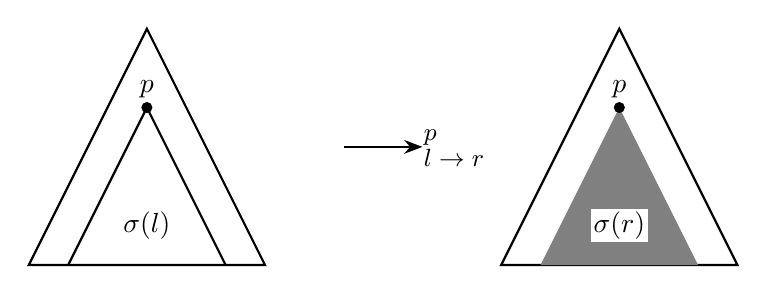
\begin{tikzpicture}[sibling distance=5em]
  \draw [thick] (0,0) -- +(3,0) -- +(1.5,3) -- cycle;
  \draw [thick] (0.5,0) -- +(1,2) -- +(2,0);

  \fill (1.5,2) circle [radius=2pt] node [above] {$p$};
  \draw (1.5,0.5) node {$\sigma(l)$};

  \draw [-{Stealth},thick] (4,1.5) -- +(1,0);
  \draw (5.1,1.4) node [above=0pt] {\small $p$};
  \draw (5.4,1.6) node [below=0pt] {\small $l\ra r$};

  \begin{scope}[xshift=60mm]
    \draw [thick] (0,0) -- +(3,0) -- +(1.5,3) -- cycle;
    \fill [gray] (0.5,0) -- +(1,2) -- +(2,0) -- cycle;

    \fill (1.5,2) circle [radius=2pt] node [above] {$p$};
    \draw (1.5,0.5) node [inner sep=1pt,fill=white] {$\sigma(r)$};
  \end{scope}  

\end{tikzpicture}
\caption{重写的树视图}
\label{f:rewriting}
\end{figure}

\begin{example}
利用例~\ref{e:add} 的重写模型$\cR$,可以得到以下重写序列,其中被重写替换的子项表达式(即重写规则左项的实例)用下划线标出:
\begin{eqnarray}
t_1 & = & \underline{\add(\s(\zero),\zero)} \lrps{}{} \s(\underline{\add(\zero,\zero)}) \lrps{}{} \s(\zero) \;\; ;\nonumber \\
t _2 & = & \underline{\add(\s^2(\zero),\s(\zero))} \lrps{}{} \s(\underline{\add(\s(\zero),\s(\zero))}) \nonumber\\ 
& & \lrps{}{} \s^2(\underline{\add(\zero,\s(\zero))}) \lrps{}{} \s^2(\s(\zero)) \;\; .\nonumber 
\end{eqnarray}
\end{example}

从上例不难看出,例~\ref{e:add} 的重写模型$\cR$定义了自然数加法的计算方式,即通过重写规则赋予了抽象函数符号$\add$自然数加法的语义。由于$\cR$不满足自然数乘法的性质,因此无法将$\add$解释为自然数乘法符号。因此,重写模型通过重写规则给函数符号赋予语义。

重写可以看作一种计算,也可以看作一种关系。

\begin{definition}[重写关系]
给定定义在词汇表$\cF$上的重写模型$\cR$,$\cR$对应的重写关系$\lrps{}{\cR}$定义为$\TFX$上的二元关系:
\begin{eqnarray}
\lrps{}{\cR} & \defeq & \{ \lb u,v\rb 
\mid \mbox{存在$p$和$(l\ra r)\in\cR$,满足$u\lrps{p}{l\ra r}v$}\}  \nonumber 
\end{eqnarray}
给定重写关系 $\lrps{}{\cR}$,它的对称闭包记作$\eqps{}{\cR}$,自反传递闭包记作 
$\lrps{*}{\cR}$,自反对称传递闭包记作$\eqps{*}{\cR}$。
\end{definition}

重写是一种\emph{非确定}的技术。重写的非确定性体现在两个方面:(1) 给定项表达式$t$,重写发生的位置$p$允许是任意的;(2) 给定项表达式$t$,重写应用的重写规则$l \ra r$允许是任意的。例如在例~\ref{e:nondet} 中,从项表达式$t$出发,产生了两条不同的重写序列。第一条序列先在位置$\rootp$(即树的根结点)进行重写,然后继续在位置$\rootp$进行重写;第二条序列则先在位置$2$(即根结点的第2个子结点)进行重写,然后继续在位置$\rootp$进行重写。

\begin{example}
\label{e:nondet}
利用例~\ref{e:add} 的重写模型$\cR$,可以得到以下重写序列:
\begin{eqnarray}
t & = & \underline{\add(\zero,\add(\zero,x))} \lrps{\rootp}{} 
\underline{\add(\zero,x)} \lrps{\rootp}{} x \nonumber \\
t & = & \add(\zero,\underline{\add(\zero,x)}) \lrps{2}{} 
\underline{\add(\zero,x)} \lrps{\rootp}{} x \nonumber 
\end{eqnarray}
\end{example}

重写过程不一定是终止的,即某项表达式$t$可以一直被重写,其过程不会停止。如例~\ref{e:nonter},利用重写模型$\cR_1$,可以得到无穷的重写序列$a\lrps{}{\cR_1}a\lrps{}{\cR_1} a \lrps{}{\cR} \ldots$;利用重写模型$\cR_2$,可以得到无穷的重写序列$f(a,b) \lrps{}{\cR_2} f(b,a) \lrps{}{\cR_2} f(a,b) \lrps{}{\cR_2} \ldots$。

\begin{example}
\label{e:nonter}
给定$\cF_1=\{a^{(0)}\}$,定义
\begin{eqnarray}
\cR_1 & = & \{a \ra a\} \; ; \nonumber
\end{eqnarray}
给定$\cF_2=\{a^{(0)},b^{(0)},f^{(2)}\}$,定义
\begin{eqnarray}
\cR_2 & = & \{f(x,y) \ra f(y,x)\} \; ; \nonumber
\end{eqnarray}
\end{example}

\begin{definition}[终止性]
\label{d:termination}
给定重写关系$\lrps{}{\cR}$,如果对任意项表达式$t$都不存在无穷的重写序列$t\lrps{}{\cR} t_1 \lrps{}{\cR} t_2 \lrps{}{\cR} \ldots$,则称重写关系$\lrps{}{\cR}$是终止的。重写模型$\cR$是终止的,当且仅当重写关系$\lrps{}{\cR}$是终止的。
\end{definition}

\begin{definition}[范式]
\label{d:normalform}
给定重写模型$\cR$,如果项表达式$s$无法应用任意重写规则$(l \ra r)\in \cR$进行重写,则称$s$是(关于$\cR$的)范式。
\end{definition}

\begin{lemma}
如果重写模型$\cR$是终止的,那么对任意项表达式$t\in\TFX$,存在范式$s\in\TFX$满足$t\lrps{*}{\cR} s$。此时称$s$是$t$(关于$\cR$)的范式,重写序列$t\lrps{*}{\cR} s$可记作$t\lrps{!}{\cR} s$。求范式的过程称作\emph{规范化}。
\end{lemma}

重写的终止性是重写领域研究的重要问题之一。给定任意一个重写模型$\cR$,判定$\cR$是否终止的问题,是一个\emph{不可判定}的问题~\cite{DBLP:conf/rta/Dauchet89,tech1978}。重写模型的终止性问题不是本文讨论的内容,在此不详述,更多探讨可参考~\inlinecite{terese,DBLP:conf/rta/1995,DBLP:journals/iandc/GeserHWZ07,DBLP:journals/tcs/Payet08,DBLP:journals/tcs/Lescanne94,DBLP:conf/tlca/JouannaudL15}。

由于重写的非确定性,即使重写模型是终止的,任意项表达式的范式也不一定是唯一的。如例~\ref{e:diffnorm},根据$\cR$,有$a\lrps{!}{\cR} b$以及$a \lrps{!}{\cR}c$,即$b$和$c$都是关于$\cR$的$a$的范式,可见$a$的范式并不唯一。

\begin{example}
\label{e:diffnorm}
给定$\cF=\{a^{(0)},b^{(0)},c^{(0)}\}$,定义
\begin{eqnarray}
\cR & = & \{a \ra b\; , a\ra c\} \; \mbox{。} \nonumber
\end{eqnarray}
\end{example}

\begin{definition}[合流性]
\label{d:confluence}
给定重写关系$\lrps{}{\cR}$,如果对任意满足$u\rlps{*}{\cR} s \lrps{*}{\cR} v$的项表达式$s,u,v$,都存在$t$使$u\lrps{*}{\cR} t \rlps{*}{\cR} v$,则称$\lrps{}{\cR}$是合流的。重写模型$\cR$是合流的,当且仅当重写关系$\lrps{}{\cR}$是合流的。
\end{definition}

重写的合流性也是重写领域研究的重要问题之一。给定任意一个重写模型$\cR$,判定$\cR$是否合流的问题,也是一个不可判定的问题~\cite{DBLP:journals/ipl/Jacquemard03}。与终止性类似,重写模型的合流性问题不是本文讨论的内容,在此不详述,更多探讨可参考~\inlinecite{terese,newman42,hindley1964church,DBLP:journals/jacm/Rosen73,knuth70,DBLP:conf/rta/Oostrom08,DBLP:journals/jar/ZanklFM15,DBLP:conf/csl/LiuJO15,DBLP:conf/rta/LiuDJ14}。

把重写看作计算的过程,终止性保证计算结果存在,而合流性保证计算结果唯一,即计算过程的非确定性不影响计算结果的确定性。

\begin{lemma}
如果重写模型$\cR$是终止的且合流的,那么任意项表达式$t$关于$\cR$的范式存在且唯一,记作$\nf{t}{\cR}$。在$\cR$已知的情况下,简记作$\nf{t}{}$。
\end{lemma}



\subsection{等式规则与等价关系}

重写规则是有方向性的,因此重写是不可逆的过程。给定$s\lrps{}{\cR}t$,$s$和$t$处于不等价的关系。然而在某些情况下,我们需要描述两个项表达式之间等价的关系。例如针对例~\ref{e:add} 的重写模型,项表达式$\add(x,\zero)$已经是自身的范式,$\add(x,\zero) = \nf{\add(x,\zero)}{}$。但正如之前的描述,我们想赋予$\add$自然数加法的语义。我们知道交换律是自然数加法具有的性质,在此意义上,我们认为项表达式$\add(x,\zero)$应该可以进一步化简为$x$。因此交换律的语义应该以形如$\add(x,y)\ra\add(y,x)$的重写规则被加入到该重写模型中。然而,从例~\ref{e:nonter} 的$\cR_2$可以看出,这种形式的重写规则会破坏重写模型的终止性。

为此,需要引入等式规则与等价关系的概念。

\begin{definition}[等式规则]
\label{d:eq}
给定词汇表$\cF$,一条等式规则是由项表达式$l,r\in\TFX$组成的无序对(无序二元组),记作$l\sim r$。
\end{definition}

\begin{definition}[等价模型]
\label{d:eq-sys}
给定词汇表$\cF$,等价模型是一个由若干等式规则组成的集合$\cE = \{l_i \sim r_i\}_i$。
\end{definition}

由于等式规则是无序对,因此$l\sim r$等同于$r\sim l$。$(l\sim r)\in\cE$当且仅当$(r\sim l)\in\cE$。

\begin{example}
\label{e:add-ac}
假定$\cF = \{\add^{(2)}\}$。可定义以下等价模型:
\begin{eqnarray}
\cE = \{ &  & \add(x, y) \sim \add(y,x) \; , \nonumber \\
         &  & \add(\add(x,y), z) \sim \add(x,\add(y,z)) \;\;\; \}\mbox{。} \nonumber
\end{eqnarray}
\end{example}

例~\ref{e:add-ac} 的规则分别定义了函数符号$\add$的交换律和结合律。

应用等式规则的方式与应用重写规则的方式类似:

\begin{definition}[等价]
\label{d:equality}
给定等价模型$\cE$,项表达式$u,v\in\TFX$,位置$p\in\Pos{u}$,等式规则$(l \sim r) \in \cE$。如果存在代换$\sigma$满足$u|_p = \sigma(l)$以及$v=u[\sigma(r)]_p$,则称$u$和$v$在位置$p$关于等式规则$l\sim r$等价,记作$u\eqps{p}{l\sim r} v$。记号中的$p$和$l\sim r$可忽略不写。
\end{definition}

记号$\eqps{}{}$表明了应用等式规则的过程是个对称、可逆的过程。

\begin{example}
利用例~\ref{e:add-ac} 的等价模型,可得到以下等价序列:
\begin{eqnarray}
& & \add(\add(x,y),z) \eqps{1}{} \add(\add(y,x),z) \eqps{\rootp}{} \add(y,\add(x,z)) \eqps{\rootp}{} \add(\add(x,z),y) \mbox{。}\nonumber 
\end{eqnarray}
\end{example}

\begin{definition}[等价关系]
\label{d:equiv}
给定定义在词汇表$\cF$上的等价模型$\cE$,$\cE$对应的等价关系$\eqps{}{\cE}$定义为$\TFX$上的二元关系:
\begin{eqnarray}
\eqps{}{\cE} & \defeq & \{ \lb u,v\rb 
\mid \mbox{存在$p$和$(l\sim r)\in\cE$,满足$u\eqps{p}{l\sim r}v$}\}  \nonumber 
\end{eqnarray}
给定等价关系 $\eqps{}{\cE}$,它的对称闭包是它自身,自反传递闭包记作 
$\eqps{*}{\cE}$。
\end{definition}

由于等价关系是对称的,任意等价关系$u\eqps{}{\cE}v$都可以扩展成一个无穷等价序列$u\eqps{*}{\cE}v$。因此区分等价关系$\eqps{}{\cE}$及其自反传递闭包$\eqps{*}{\cE}$并无意义。我们将$u\eqps{*}{\cE}v$记作$u=_{\cE}v$。

\section{重写模型的扩展}

\subsection{模重写}

等价关系为抽象的函数符号赋予了“等价”的语义。等价关系的引入,是为了增强重写的能力。\emph{模重写}技术的目的就是定义一种二者融合的方式。

\begin{definition}[模重写模型]
\label{d:rewsys-modulo}
给定词汇表$\cF$,模重写模型是一个由重写模型$\cR$和等价模型$\cE$组成的有序对(二元组),记作$\cR_{\cE} \defeq \lb \cR, \cE \rb$。
\end{definition}

\begin{definition}[模重写]
\label{d:rewriting-modulo}
给定模重写模型$\RE$,项表达式$u,v\in\TFX$,位置$p\in\Pos{u}$,重写规则$(l \ra r) \in \cR$。如果存在代换$\sigma$满足$u|_p =_{\cE} \sigma(l)$以及$v=u[\sigma(r)]_p$,则称$u$在位置$p$应用重写规则$l\ra r$模重写为$v$,记作$u\lrps{p}{(l\ra r)_{\cE}} v$。记号中的$p$和$(l\ra r)_{\cE}$可忽略不写。
\end{definition}

重写技术替换的是项表达式$u$中存在的规则左项的实例$\sigma(l)$,而模重写技术替换的则是$u$中与规则左项实例$\sigma(l)$关于$\cE$等价的子项表达式。这使得重写过程得以“利用”各函数符号的等价语义。

\begin{example}
\label{e:add-ac-mod}
假定$\cF = \{\zero^{(0)}, \s^{(1)}, \add^{(2)}\}$。可定义模重写模型$\RE$,其中:
\begin{eqnarray}
\cR = \{ &  & \add(\zero, y) \ra y \; , \nonumber \\
         &  & \add(\s(x), y) \ra \s(\add(x,y)) \;\;\; \}\;\; ; \nonumber \\
\cE = \{ &  & \add(x, y) \sim \add(y,x) \; , \nonumber \\
         &  & \add(\add(x,y), z) \sim \add(x,\add(y,z)) \;\;\; \}\mbox{。} \nonumber         
\end{eqnarray}
可得到以下模重写序列:
\begin{eqnarray}
t_1 & = & \underline{\add(x,\s(\zero))} \lrps{}{} \s(\underline{\add(\zero,x)}) \lrps{}{} \s(x) \;\; ;\nonumber \\
t _2 & = & \underline{\add(\add(x,\s(\zero)),y)} \lrps{}{} \s(\underline{\add(\zero,\add(x,y))}) 
\lrps{}{} \s(\add(x,y)) \;\; \mbox{。}\nonumber 
\end{eqnarray}
\end{example}

类似于重写,我们可以定义模重写对应的模重写关系、终止性、范式和合流性。

\begin{definition}[模重写关系]
给定定义在词汇表$\cF$上的模重写模型$\RE$,$\RE$对应的模重写关系$\lrps{}{\RE}$定义为$\TFX$上的二元关系:
\begin{eqnarray}
\lrps{}{\RE} & \defeq & \{ \lb u,v\rb 
\mid \mbox{存在$p$和$(l\ra r)\in\cR$,满足$u\lrps{p}{(l\ra r)_{\cE}}v$}\}  \nonumber 
\end{eqnarray}
给定模重写关系 $\lrps{}{\RE}$,它的对称闭包记作$\eqps{}{\RE}$,自反传递闭包记作 
$\lrps{*}{\RE}$,自反对称传递闭包记作$\eqps{*}{\RE}$。
\end{definition}

\begin{definition}
给定模重写关系$\lrps{}{\RE}$,如果对任意项表达式$t$都不存在无穷的模重写序列$t\lrps{}{\RE} t_1 \lrps{}{\RE} t_2 \lrps{}{\RE} \ldots$,则称模重写关系$\lrps{}{\RE}$是终止的。模重写模型$\RE$是终止的,当且仅当模重写关系$\lrps{}{\RE}$是终止的。
\end{definition}

\begin{definition}
给定模重写模型$\RE$,如果项表达式$s$无法应用任意重写规则$(l \ra r)\in \cR$进行模重写,则称$s$是(关于$\RE$的)范式。
\end{definition}

\begin{lemma}
如果模重写模型$\RE$是终止的,那么对任意项表达式$t\in\TFX$,存在范式$s\in\TFX$满足$t\lrps{*}{\RE} s$。此时称$s$是$t$(关于$\RE$)的范式,模重写序列$t\lrps{*}{\RE} s$可记作$t\lrps{!}{\RE} s$。
\end{lemma}

\begin{definition}
给定模重写关系$\lrps{}{\RE}$,如果对任意满足$u\rlps{*}{\RE} s \lrps{*}{\RE} v$的项表达式$s,u,v$,都存在$t$和$t'$使$u\lrps{*}{\RE} t =_{\cE} t' \rlps{*}{\RE} v$,则称$\lrps{}{\RE}$是合流的。模重写模型$\RE$是合流的,当且仅当模重写关系$\lrps{}{\RE}$是合流的。
\end{definition}

\begin{lemma}
如果模重写模型$\RE$是终止的且合流的,那么任意项表达式$t$关于$\RE$的范式存在且关于$\cE$等价。也就是说,如果$t\lrps{!}{\RE} s_1$,$t\lrps{!}{\RE} s_2$,那么$s_1 =_{\cE} s_2$。 此时也可称$t$关于$\RE$的范式关于$=_{\cE}$唯一,将任一范式记作$\nf{t}{\RE}$。在$\RE$已知的情况下,简记作$\nf{t}{}$。
\end{lemma}

模重写技术可以看作是将重写技术中的语法等价(相等关系$=$)扩展为语义等价(等价关系$=_{\cE}$)。重写模型是模重写模型的等价关系$=_{\cE}$为空时的特殊情况,即$\cR = \cR_{\emptyset}$。关于模重写的终止性和合流性的研究,可参考\inlinecite{terese,DBLP:conf/cade/JouannaudM84,DBLP:journals/tcs/JouannaudM92,DBLP:journals/ijsi/JouannaudT08,DBLP:conf/rta/Jouannaud06,DBLP:journals/tcs/JouannaudL12,DBLP:journals/siamcomp/JouannaudK86}。


\subsection{条件重写}

对于标准的重写技术,触发重写的条件是通过模式匹配体现的。假如给定形如$f(x)$的项表达式,我们希望当$x\ge 2$时,$f(x)$可以重写为$a$;当$x<2$时,$f(x)$可以重写为$b$。那么根据例~\ref{e:add},我们需要增加如下规则:
\begin{eqnarray}
f(\s^2(x)) & \ra & a \nonumber \\
f(\zero)  & \ra & b \nonumber \\
f(\s(\zero)) & \ra & b \nonumber
\end{eqnarray}
如果判断是否满足$x\ge 3$,则右项为$b$的规则需要增加至3条;以此类推,如果判断是否满足$x\ge n$,右项为$b$的规则需要增加至n条。这就给设计规则的过程带来极大不便。

给重写规则增加条件约束,则可以大大地增加重写规则的表达能力。例如我们希望可以通过以下形式的规则来表示上述的情况:
\begin{eqnarray}
f(x) & \ra & a ~~\mbox{ if }~~ x\ge \s^2(\zero) \nonumber \\
f(x)  & \ra & b ~~\mbox{ if }~~ x < \s^2(\zero) \nonumber 
\end{eqnarray}

\begin{definition}[条件重写规则]
\label{d:crule}
给定词汇表$\cF$,条件重写规则由重写规则和若干等式构成,形如
\begin{eqnarray}
l \ra r & \Dla & u_1 = v_1 \land \ldots \land u_n = v_n \;\; ,\nonumber
\end{eqnarray}
其中$l,r\in\TFX$,对$1\le i\le n$有$u_i,v_i\in\TFX$。其中$l$称作该条件重写规则的左项,$r$称作该条件重写规则的右项,$u_i = v_i$称作该条件重写规则的条件约束。
\end{definition}

\begin{definition}[条件重写模型]
\label{d:crewrite-sys}
给定词汇表$\cF$,条件重写模型是一个由若干条件重写规则组成的集合$\cR = \{l_i \ra r_i \Dla C_i \}_i$。
\end{definition}

\begin{example}
\label{e:cond}
假定$\cF = \{\zero^{(0)}, \s^{(1)}, \add^{(2)}, f^{(2)}, a^{(0)}, b^{(0)}, \true^{(0)}, \false^{(0)}, \mynot^{(1)}, \lessthan^{(2)} \}$。可定义以下条件重写模型:
\begin{eqnarray}
\cR = \{ &  & f(x) \ra a \;\Dla\; \mynot(\lessthan(x,\s^2(\zero))) = true \; , \nonumber \\
         &  & f(x) \ra b \;\Dla\; \lessthan(x,\s^2(\zero)) = ture \;\;\;\;\; \}\mbox{。} \nonumber
\end{eqnarray}
\end{example}

例~\ref{e:cond} 中的两条规则对应了本小节开头提出的重写需求。

虽然我们给出了条件重写规则的形式,但是其语义并不清晰。条件重写规则里的条件约束$u_i=v_i$,是代表$u_i$和$v_i$语法上的相等呢?是代表$u_i\eqps{*}{}v_i$呢?是代表存在$t$使$u_i\lrps{*}{}t\rlps{*}{}v_i$呢?还是$u_i\lrps{*}{}v_i$呢?关于条件约束的不同语义解释有多种讨论~\cite{brand1978completeness,DBLP:journals/jcss/BergstraK86,DBLP:conf/cade/DershowitzOS88},这里我们采用最常用的实现方法:
存在$t$使$u_i\lrps{*}{}t\rlps{*}{}v_i$。

\begin{definition}[条件重写]
\label{d:crewriting}
给定条件重写模型$\cR$,项表达式$u,v\in\TFX$,位置$p\in\Pos{u}$,条件重写规则$(l \ra r \Dla C_i) \in \cR$。如果存在代换$\sigma$满足$u|_p = \sigma(l)$,$v=u[\sigma(r)]_p$,以及对任意$(u_j = v_j)\in C_i$存在$t_j$使$u_j\lrps{*}{} t_j \rlps{*}{} v_j$, 则称$u$在位置$p$应用条件重写规则$l\ra r \Dla C_i$重写为$v$,记作$u\lrps{p}{l\ra r} v$。记号中的$p$和$l\ra r$可忽略不写。
\end{definition}

条件重写的意思是,被重写的子项表达式不仅需要是重写规则左项$l$的实例,且其对应的代换$\sigma$需要满足该规则的所有条件约束。

针对例~\ref{e:cond},为了实现条件约束的求解,还需要加入以下规则:
\begin{eqnarray}
\lessthan(x,\zero) & \ra & \false \nonumber \\
\lessthan(\zero,\s(y)) & \ra & \true \nonumber \\
\lessthan(\s(x),\s(y)) & \ra & \lessthan(x,y) \nonumber \\
\mynot(\false) & \ra & \true \nonumber \\
\mynot(\true) & \ra & \false \;\;\mbox{。} \nonumber 
\end{eqnarray}

重写模型对应于条件重写模型中所有条件约束均为空的特殊情况。重写模型的相关概念,包括重写关系、终止性、范式及合流性,均可自然地扩展成条件重写模型的对应概念,在此不再赘述。给定任意模重写模型$\RE$,将其中的重写模型$\cR$替换成条件重写模型,则得到\emph{条件模重写}模型及其相关概念。


\section{规范化条件重写模型}

在模重写和条件重写的基础上,本文提出一种新的重写模型扩展,叫\emph{规范化条件重写模型}。

条件重写模型在应用某条重写规则时,需要判断其条件约束是否成立,即是否存在$t$使$u_i\lrps{*}{}t\rlps{*}{}v_i$,这个过程是不可判定的~\cite{DBLP:journals/ipl/Jacquemard03}。理想的做法是通过$u_i$和$v_i$的范式来确定条件是否成立,即判断是否有${\nf{u_i}{}} = {\nf{v_i}{}}$。此时,只需要在语法上判断是否相等即可。这就要求该条件重写模型是终止的,或者至少要求用于求范式的重写规则是终止的~\cite{DBLP:conf/cade/DershowitzOS88,DBLP:journals/tcs/DershowitzO90,DBLP:conf/rta/BertlingG89}。另一方面,在例~\ref{e:cond} 中,注意到用于求解条件约束的规则与描述需求的规则(即$f(x)\ra a$与$f(x)\ra b$)相对独立。规则$f(x)\ra a$和$f(x)\ra b$用于赋予模型语义,而其它规则则用于辅助定义$f(x)\ra a$和$f(x)\ra b$。这当中存在层次关系,而属于同一个重写规则集使得该有的区别模糊不清,这从概念上和技术上都是欠妥的。

本文提出的规范化(条件)重写模型,则是基于上述考虑,将(条件)模重写模型进一步划分层次。


\begin{definition}[规范化重写模型]
\label{d:normalrew-sys}
给定词汇表$\cF$,规范化重写模型是一个由重写模型$\cR,\cS$和等价模型$\cE$组成的三元组,记作$\RSE \defeq \lb \cR, \cS, \cE \rb$。其中由$\cS$和$\cE$组成的模重写模型$\SE$必须满足终止性和合流性。
\end{definition}

重写不一定是终止的,因此不能将任意重写模型的重写过程看作是化简的过程。例如规则$a\ra f(a)$会将项表达式$a$重写为更加复杂的表达式。但是当重写模型具有终止性时,重写过程就可以看作是一个化简的过程。规范化重写模型$\RSE$要求$\SE$是终止且合流的,使得$\SE$可看作一个良定义的化简函数:计算结果(范式)存在且唯一。因此,重写模型$\cS$可称作\emph{化简模型},其对应的重写规则可称作\emph{化简规则}。

\begin{definition}[规范化重写]
\label{d:normalrewriting}
给定规范化重写模型$\RSE$,项表达式$u,v\in\TFX$,重写规则$(l \ra r) \in \cR$。如果存在位置$p$和项表达式$s,t$满足
${\nf{u}{\SE}} =_{\cE} s \lrps{p}{l\ra r} t$且$v = {\nf{t}{\SE}}$,则称$u$应用重写规则$l\ra r$规范化重写为$v$,记作$u\lrps{}{(l\ra r)_{\cS\cE}} v$。记号中的$(l\ra r)_{\cS\cE}$在不存在二义性时可忽略不写。
\end{definition}

简单地说,如果$u\lrps{}{(l\ra r)_{\cS\cE}}v$,则$u$和$v$之间存在关系
$u \lrps{!}{\SE} {\nf{u}{\SE}} =_{\cE} s \lrps{p}{l\ra r} t \lrps{!}{\SE} {\nf{t}{\SE}} = v$。从技术上看,给定项表达式$u$,要想对$u$进行规范化重写,需要先对$u$进行规范化,得到$u$关于$\SE$的范式$\nf{u}{\SE}$。然后在$\nf{u}{\SE}$关于$=_{\cE}$的等价类中选定项表达式$s$,对其进行重写得到项表达式$t$。最后对$t$进行规范化得到其关于$\SE$的范式$\nf{t}{\SE}$。

规范化重写技术在应用重写规则前,要求项表达式必须是范式。在应用重写规则后,又显式地进行规范化,使最终得到的项表达式成为范式。这就保证对于任意规范化重写序列$u_0 \lrps{}{} u_1 \lrps{}{} \ldots \lrps{}{} u_n$,对任意$i\in [1,n]$满足$u_i$是关于$\SE$的范式,即重写序列中的项表达式始终处于“最简”形式。

规范化重写模型通过对规则分类,使模型的语义更加清晰:$\cE$描述与等价相关的语义,$\cS$描述与函数计算、形式简化相关的语义,$\cR$描述最核心的、用户关心的语义。

\begin{example}
\label{e:river}
假定$\cF = \{\comp^{(2)}, \farmer^{(1)}, \wolf^{(1)}, \lamb^{(1)}, \grass^{(1)}, \lhs^{(0)}, \rhs^{(0)}, \change^{(1)} \}$,其中函数符号$\comp$采用中缀记法,即$x\comp y$表示$\comp(x,y)$。可定义规范化重写模型$\RSE$,其中:
\begin{eqnarray}
\cE = \{ &  & x\comp y \sim y\comp x \; , \nonumber \\
         &  & (x\comp y) \comp z \sim x \comp (y\comp z)  \;\;\;\;\; \} \; ; \nonumber \\
\cS = \{ &  & \change(\lhs) \ra \rhs \; , \nonumber \\
         &  & \change(\rhs) \ra \lhs \;\;\;\;\; \} \; ; \nonumber \\
\cR = \{ &  & \farmer(x) \ra_1 \farmer(\change(x)) \; , \nonumber \\
         &  & \farmer(x)\comp \wolf(x) 
         \ra_2 \farmer(\change(x))\comp\wolf(\change(x)) \; , \nonumber \\
         &  & \farmer(x)\comp \lamb(x) 
         \ra_3 \farmer(\change(x))\comp\lamb(\change(x)) \; , \nonumber \\ 
         &  & \farmer(x)\comp \grass(x) 
         \ra_4 \farmer(\change(x))\comp\grass(\change(x)) \; \} \mbox{。}\nonumber
\end{eqnarray}
可得到以下规范化重写序列:
\begin{eqnarray}
t & = & \farmer(\lhs) \comp \wolf(\lhs) \comp 
        \lamb(\lhs) \comp \grass(\lhs) \nonumber \\
  & \lrps{}{3} & \farmer(\rhs) \comp \lamb(\rhs) \comp 
        \wolf(\lhs) \comp \grass(\lhs) \nonumber \\
  & \lrps{}{1} & \farmer(\lhs) \comp \lamb(\rhs) \comp 
        \wolf(\lhs) \comp \grass(\lhs) \nonumber \\
  & \lrps{}{2} & \farmer(\rhs) \comp \wolf(\rhs) \comp 
        \lamb(\rhs) \comp \grass(\lhs) \nonumber \\    
  & \lrps{}{3} & \farmer(\lhs) \comp \lamb(\lhs) \comp 
        \wolf(\rhs) \comp \grass(\lhs) \nonumber \\    
  & \lrps{}{4} & \farmer(\rhs) \comp \grass(\rhs) \comp 
        \wolf(\rhs) \comp \lamb(\lhs) \nonumber \\     
  & \lrps{}{1} & \farmer(\lhs) \comp \grass(\rhs) \comp 
        \wolf(\rhs) \comp \lamb(\lhs) \nonumber \\                  
  & \lrps{}{3} & \farmer(\rhs) \comp \lamb(\rhs) \comp 
        \wolf(\rhs) \comp \grass(\rhs) \; \mbox{。} \nonumber
\end{eqnarray}
\end{example}

例~\ref{e:river} 描述的是农夫过河的问题。$\lhs$和$\rhs$分别表示河的左岸和右岸;$\farmer(x)$、$\wolf(x)$、$\lamb(x)$和$\grass(x)$分别表示农夫、狼、羊和草当前所处位置为河的$x$岸;$\change(x)$表示$x$岸的对岸;$\comp$作为连接符构成农夫、狼、羊和草在任一时刻的状态,如$\farmer(\lhs) \comp \lamb(\lhs) \comp \wolf(\rhs) \comp \grass(\lhs)$
表示当前状态为农夫在左岸、羊在左岸、狼在右岸、草在左岸。$\cE$的等价规则分别表示函数符号$\comp$具有交换律和结合律,因此$\comp$连接的多个项表达式构成了一个多重集合,其中的括号可以省略。$\cS$的重写规则定义了化简$\change$的方式。$\cR$的四条规则定义了系统状态发生改变的四种方式:(1) 农夫独自一人过河;(2) 农夫带着狼过河;(3) 农夫带羊过河;(4) 农夫带草过河。$\cR$的规则用数字进行了编号。例~\ref{e:river} 的重写序列描述了一种可能的方案,从农夫、狼、羊和草都处于左岸的初始状态,变成四者都处于右岸的状态。序列中用右箭头的数字下标表示规范化重写应用的规则编号。

\begin{definition}[规范化重写关系]
给定定义在词汇表$\cF$上的规范化重写模型$\RSE$,$\RSE$对应的规范化重写关系$\lrps{}{\RSE}$定义为$\TFX$上的二元关系:
\begin{eqnarray}
\lrps{}{\RSE} & \defeq & \{ \lb u,v\rb 
\mid \mbox{存在$(l\ra r)\in\cR$,满足$u\lrps{}{(l\ra r)_{\cS\cE}}v$}\}  \nonumber 
\end{eqnarray}
给定规范化重写关系 $\lrps{}{\RSE}$,它的对称闭包记作$\eqps{}{\RSE}$,自反传递闭包记作 
$\lrps{*}{\RSE}$,自反对称传递闭包记作$\eqps{*}{\RSE}$。
\end{definition}

类似地,条件约束可以增加规范化重写模型的表达能力,扩展得到\emph{规范化条件重写模型}。


\begin{definition}[规范化条件重写模型]
\label{d:cnormalrew-sys}
给定词汇表$\cF$,规范化条件重写模型是一个由条件重写模型$\cR,\cS$和等价模型$\cE$组成的三元组,记作$\RSE \defeq \lb \cR, \cS, \cE \rb$。其中由$\cS$和$\cE$组成的条件模重写模型$\SE$必须满足终止性和合流性。
\end{definition}

上文已经提到,条件重写模型是重写模型的一种自然扩展。规范化条件重写模型仅仅是将规范化重写模型$\lb \cR, \cS, \cE\rb$中的标准重写模型$\cR$和$\cS$扩展为条件重写模型,且同样对$\SE$的终止性和合流性有要求。

虽然在形式上看,规范化条件重写模型只是简单地将重写规则替换为条件重写规则。但从语义解释上,却与简单的替换有所不同。

\begin{definition}[规范化条件重写]
\label{d:cnormalrewriting}
给定规范化条件重写模型$\RSE$,项表达式$u,v\in\TFX$,条件重写规则$(l \ra r \Dla C_i) \in \cR$。如果存在位置$p$、代换$\sigma$和项表达式$s,t$满足:
\begin{enumerate}[(i)]
\item ${\nf{u}{\SE}} =_{\cE} s$;    
\item $s|_p = \sigma(l)$,$t = s[\sigma(r)]_p$;
\item 对任意$(u_j = v_j)\in C_i$,存在$w_j$使$u_j\lrps{*}{\SE} w_j \rlps{*}{\SE} v_j$;
\item $v = {\nf{t}{\SE}}$;
\end{enumerate}
则称$u$应用条件重写规则$l\ra r \Dla C_i$规范化条件重写为$v$,记作$u\lrps{}{(l\ra r)_{\cS\cE}} v$。记号中的$(l\ra r)_{\cS\cE}$在不存在二义性时可忽略不写。
\end{definition}
 

与规范化重写类似,如果$u\lrps{}{(l\ra r)_{\cS\cE}}v$,则$u$和$v$之间存在关系
$u \lrps{!}{\SE} {\nf{u}{\SE}} =_{\cE} s \lrps{p}{l\ra r} t \lrps{!}{\SE} {\nf{t}{\SE}} = v$。
但需要注意其中的条件重写步骤$s\lrps{p}{l\ra r}t$,它判断条件约束$u_j=v_j$是否成立时,不是递归地使用模型$\RSE$,而是直接使用$\SE$。也就是说,$u_j$和$v_j$需要满足
$u_j\lrps{*}{\SE} w_j \rlps{*}{\SE} v_j$而不是$u_j\lrps{*}{\RSE} w_j \rlps{*}{\RSE} v_j$。由于条件模重写模型$\SE$是终止且合流的,$u_j\lrps{*}{\SE} w_j \rlps{*}{\SE} v_j$可以进一步简化为${\nf{u_j}{\SE}} =_{\cE} {\nf{v_j}{\SE}}$,这就在一定程度上解决了本小节开头提出的不可判定性问题,使规范化条件重写从技术上可以被实现。

与规范化重写类似,从技术上看,规范化条件重写也必须经过规范化、条件重写、规范化三个过程。这保证了规范化条件重写序列中的任意项表达式都始终处于“最简”形式。

\begin{definition}[规范化条件重写关系]
给定定义在词汇表$\cF$上的规范化条件重写模型$\RSE$,$\RSE$对应的规范化条件重写关系$\lrps{}{\RSE}$定义为$\TFX$上的二元关系:
\begin{eqnarray}
\lrps{}{\RSE} & \defeq & \{ \lb u,v\rb 
\mid \mbox{存在$(l\ra r)\in\cR$,满足$u\lrps{}{(l\ra r)_{\cS\cE}}v$}\}  \nonumber 
\end{eqnarray}
给定规范化条件重写关系 $\lrps{}{\RSE}$,它的对称闭包记作$\eqps{}{\RSE}$,自反传递闭包记作 
$\lrps{*}{\RSE}$,自反对称传递闭包记作$\eqps{*}{\RSE}$。
\end{definition}

\begin{example}
\label{e:cnormalrew}
假定$\cF = \{\zero^{(0)}, \s^{(1)}, f^{(2)}, a^{(0)}, b^{(0)}, \true^{(0)}, \false^{(0)}, \mynot^{(1)}, \lessthan^{(2)} \}$。可定义规范化条件重写模型$\RSE$,其中:
\begin{eqnarray}
\cE = \phantom{\{} & & \emptyset \; ; \nonumber \\
\cS = \{ & & \lessthan(x,\zero)  \ra  \false \; , \nonumber \\
         & & \lessthan(\zero,\s(y))  \ra  \true \; , \nonumber \\
         & & \lessthan(\s(x),\s(y))  \ra  \lessthan(x,y) \; , \nonumber \\
         & & \mynot(\false) \ra \true \; , \nonumber \\
         & & \mynot(\true) \ra  \false \;\;\;\;\;\;\;\qquad\quad\quad\qquad\quad \} \; ; \nonumber \\
\cR = \{ &  & f(x) \ra a \;\Dla\; \mynot(\lessthan(x,\s^2(\zero))) = true \; , \nonumber \\
         &  & f(x) \ra b \;\Dla\; \lessthan(x,\s^2(\zero)) = ture \;\;\;\;\;\qquad \}\mbox{。} \nonumber
\end{eqnarray}
\end{example}

例~\ref{e:cnormalrew} 的规范化条件重写模型对应例~\ref{e:cond}(及其新增规则)的条件重写模型。


\begin{example}
\label{e:clock}
假定$\cF = \{\zero^{(0)}, \s^{(1)}, \add^{(2)}, \clock^{(1)}, \broken^{(0)}, \true^{(0)}, \false^{(0)}, \mynot^{(1)}, \lessthan^{(2)} \}$。可定义规范化条件重写模型$\RSE$,其中:
\begin{eqnarray}
\cE = \{ &  & \add(x, y) \sim \add(y,x) \; , \nonumber \\
         &  & \add(\add(x,y), z) \sim \add(x,\add(y,z)) \;\;\; \}\; ;
         \nonumber \\
\cS = \{ &  & \add(\zero, y) \ra y \; , \nonumber \\
         &  & \add(\s(x), y) \ra \s(\add(x,y)) \; , \nonumber \\
         & & \lessthan(x,\zero)  \ra  \false \; , \nonumber \\
         & & \lessthan(\zero,\s(y))  \ra  \true \; , \nonumber \\
         & & \lessthan(\s(x),\s(y))  \ra  \lessthan(x,y) \;\;\; \} \; ;\nonumber \\
\cR = \{ &  & \clock(x) \ra_1 \clock(\add(x,\s(\zero))) 
              \;\Dla\; \lessthan(x,\s^{11}(\zero)) = \true \; , \nonumber \\
         &  & \clock(x) \ra_2 \clock(\zero) 
              \;\Dla\; \lessthan(x,\s^{11}(\zero)) = \false \; , \nonumber \\  
         &  & \clock(x) \ra_3 \broken  
              \;\;\;\qquad\qquad\qquad\qquad\qquad\qquad\qquad\qquad\qquad \}\mbox{。} \nonumber          
\end{eqnarray}
可得到以下规范化条件重写序列:
\begin{eqnarray}
t & = & \clock(\s^0(\zero)) \lrps{}{1} \clock(\s^1(\zero))
        \lrps{}{1} \clock(\s^2(\zero))
        \lrps{}{1} \clock(\s^3(\zero)) \nonumber \\
  &   & \lrps{}{1} \ldots
        \lrps{}{1} \clock(\s^{11}(\zero))
        \lrps{}{2} \clock(\s^0(\zero))
        \lrps{}{1} \clock(\s^1(\zero))       
        \lrps{}{1} \ldots \; ;
        \nonumber \\
t & = & \clock(\s^0(\zero)) \lrps{}{1} \clock(\s^1(\zero))
        \lrps{}{1} \clock(\s^2(\zero))
        \lrps{}{3} \broken \; ; \nonumber \\
t & = & \clock(\s^0(\zero)) \lrps{}{1} \clock(\s^1(\zero))
        \lrps{}{1} \clock(\s^2(\zero))
        \lrps{}{1} \clock(\s^3(\zero)) \nonumber \\
  &   & \lrps{}{1} \ldots
        \lrps{}{1} \clock(\s^{11}(\zero))
        \lrps{}{3} \broken \; \mbox{。}
        \nonumber
\end{eqnarray}
\end{example}

例~\ref{e:clock} 描述的是一个只显示时针读数(0--11)的时钟,且这个时钟随时可能损坏。函数符号$\zero$、$\s$和$\add$用于表示自然数及自然数加法,之前已详细介绍,在此不再赘述;函数符号$\true$、$\false$分别表示命题为真和命题为假,$\mynot$表示逻辑“非”运算,$\lessthan(x,y)$表示命题“x小于y”,这四个函数符号用于定义重写规则的条件约束;$\clock(x)$表示时钟当前读数为$x$;$\broken$表示时钟当前已损坏。$\cE$的等价规则分别表示自然数加法$\add$的交换律和结合律。化简模型$\cS$包含两部分,前两条规则定义了$\add$的语义,即其计算方式;后三条规则定义了$\lessthan$的语义,即如何计算命题“x小于y”的真值。$\cR$的重写规则定义了系统状态发生改变的三种方式:规则1表示,如果时钟当前读数$x$小于11,则下一个状态的读数为$x+1$;规则2表示,如果时钟当前读数$x$不小于11,则下一个状态的读数为0(归零);规则3表示,无论时钟当前读数是多少,下一个状态时钟可能损坏。例~\ref{e:clock} 的重写序列描述了从初始状态(时钟读数为0)开始,该时钟可能发生的(其中)三种事件序列,其中箭头下标的数字表示该规范化条件重写应用的规则编号。序列1表示时钟读数从0递增至11,然后归零,周而复始,该时钟始终保持正常运作。序列2表示时钟读数从0递增至2,然后发生损坏。序列3表示时钟读数从0递增至11,然后发生损坏。

从例~\ref{e:clock} 可以看出,时钟状态是观察者关心的行为,而自然数加法、命题真值的计算只是为描述时钟状态服务,观察者并不关心。从建模的角度来看,将所有规则平等看待,非常不利于建模人员或其它模型使用者理解模型的语义。规范化条件重写模型以一种划分的方式,将模型的主要语义和辅助语义予以区分。

\section{相关工作}
\todo{进行与normalized rewriting, normal rewriting及rewriting logic的对比。}


\chapter{嵌入式系统的建模与验证}
\label{cha:modeling}

形式化模型是否适合应用于形式化建模与验证,除了取决于其自身的表达能力、验证能力外,还取决于它的易用性。不同于自动机、Petri 网等图形化模型,重写模型作为一种代数模型,其抽象的形式给建模人员的使用过程带来了额外的理解成本。本章通过提出一套针对嵌入式系统特性的建模方法,来提高规范化条件重写模型作为一种建模模型的易用性。基于语义映射,该建模方法可以在工具集 Maude 中予以实现。利用该建模方法,我们对两个真实的、经过大量测试的嵌入式系统进行了行为建模,并对其模型应用了模型检测等验证技术,成功地发现系统中存在未被测试检测到的缺陷。结果表明该方法在实际应用中具有可行性。

\section{引言}

随着嵌入式系统在生产、生活中越来越广泛的应用,嵌入式系统与我们的关系越来越紧密。特别是嵌入式系统在诸如交通运输、医疗系统、金融系统等安全攸关系统中扮演的重要角色,使其安全性、可靠性、正确性保障与我们的生命财产安全息息相关。

形式化建模与验证是提高嵌入式系统可靠性与安全性的重要方法之一。通过对嵌入式系统的行为进行建模,得到可以描述该系统行为的形式化模型。然后利用支持该模型的相关工具,对模型进行仿真、测试或形式化验证,从而检查该模型的行为是否满足开发人员的预期,进而反映原系统的行为是否满足用户的需求。

嵌入式系统的其中一个特点是具有高度并发性,这主要体现在三个方面。第一,由于嵌入式系统通常由硬件与软件协同完成其功能,硬件系统所具有的并发性不可忽视。其次,由于现代嵌入式系统处理单元逐渐变得强大,使得嵌入式软件日趋复杂。软件部分不仅仅限于完成单一任务,而且还可以搭载操作系统对复杂任务进行协调调度。软件部分的多线程进一步增加了嵌入式系统的并发性。第三,大型嵌入式系统一般由多层次构成,底层组件作为上层系统的一部分,与其它嵌入式组件协作共同完成复杂的功能,这造成了系统层面的并发性。

作为自带并发语义的一种形式化模型,重写模型及其扩展在近年来作为一种系统建模模型受到越来越多的关注,被应用到硬件描述、网络协议、安全协议等领域中~\cite{DBLP:journals/jlp/Meseguer12,DBLP:journals/iandc/MeseguerR13}。若要将其应用于嵌入式系统的实际建模验证项目,除了需要扩展现有模型提升其对软件顺序行为的描述能力外,仍需要面临两方面的挑战:
\begin{enumerate}
\item \textbf{建模方法:} 与基于状态的形式化模型(如自动机)不同,重写模型是基于抽象的项表达式与规则的。如何将重写模型的这些抽象元素与嵌入式系统的状态及复杂行为一一对应起来,需要一套系统的建模方法进行指导。
\item \textbf{工具支持:} 在根据建模方法对目标嵌入式系统进行建模,得到其对应的重写模型后,从应用的角度,我们需要一套工具支持该模型的分析与验证,否则建模毫无意义。
\end{enumerate}

本章基于第~\ref{cha:normalrewriting} 章提出的规范化条件重写模型,提出了一套系统建模方法,并针对嵌入式系统所具有的若干特性,如层次结构、高度并发、并发行为与顺序行为并存、系统结构动态变化、实时性等,将该建模方法进一步细化。基于已有的重写工具集 Maude,我们将本章提出的建模方法在 Maude 中予以实现,并通过两个真实的应用案例,验证了该方法的可行性与实用性。

本章其余部分组织结构如下:第~\ref{s:modeling-related} 小节简述基于重写模型的系统建模验证相关工作;第~\ref{s:modeling} 小节基于规范化条件重写模型,提出嵌入式系统的建模方法;第~\ref{s:tool} 小节介绍本文的建模方法如何在工具集 Maude 中予以实现;第~\ref{s:TO} 小节与~\ref{s:RMS} 小节应用本章提出的方法分别对机车优化控制系统和速率单调调度系统进行建模与验证;最后对本章内容进行简要小结。 


\section{相关工作}
\label{s:modeling-related} 

重写模型作为一种抽象的计算模型,长期以来被作为底层技术应用于定理证明器、函数式编程语言、SMT 求解器等领域中~\cite{assaf16a,DBLP:conf/lics/JouannaudO91,DBLP:conf/cav/Nadel14}。近年来,重写模型开始作为一种建模模型得到关注,并被应用于系统验证的工作中。

Bluespec 是一种基于条件重写模型的硬件描述语言~\cite{nikhil2008bluespec}。由于重写本身所具有的并发性,Bluespec 十分适用于硬件的并发行为描述。相比于 VHDL、Verilog 等传统硬件描述语言,Bluespec 以一种更加抽象的方式对目标系统行为进行描述与设计,有效提高了硬件开发效率。同时,由于 Bluespec 语言在条件重写模型的基础上支持 Haskell 的类型定义,使其对复杂类型、自定义类型的支持更加丰富。利用 Bluespec 语言编写的硬件模型支持以仿真的方式进行模型验证,Singh 和 Shukla 也提出了一套方法将 Bluespec 模型转换成 PROMELA 模型~\cite{DBLP:journals/cn/Holzmann93} 并用模型检测工具 SPIN~\cite{DBLP:journals/tse/Holzmann97} 对其进行形式化验证~\cite{DBLP:conf/mtv/SinghS07}。同时,Braibant 和 Chlipala 也提出利用交互式定理证明工具 Coq 对 Bluespec 的一个子集进行形式化验证~\cite{DBLP:conf/cav/BraibantC13}。 由于 Bluespec 是专门针对硬件设计的建模语言,因此它无法描述顺序执行的软件行为。 

重写逻辑~\cite{DBLP:journals/tcs/Marte-OlietM02,DBLP:journals/jlp/Meseguer12} 是针对建模与验证设计的一种重写模型扩展。基于重写逻辑实现的语言及工具集 Maude~\cite{DBLP:journals/tcs/ClavelDELMMQ02},以及其针对实时系统的扩展 Real-Time Maude~\cite{DBLP:journals/lisp/OlveczkyM07},支持模型仿真、可达性验证、模型检测、交互式定理证明等多种验证手段。由于重写模型的并发特点,Maude 主要被应用于生物信息、安全协议、通信协议等系统的建模与验证~\cite{DBLP:journals/jlp/Meseguer12,DBLP:journals/iandc/MeseguerR13}。Maude 的应用案例为基于重写模型的建模工作确立了一套方法框架:项表达式用于建模系统状态,重写规则用于建模系统行为~\cite{DBLP:conf/maude/2007}。 Maude 也被尝试用于软件和嵌入式系统的建模与验证工作中~\cite{DBLP:journals/scp/BaeKMO15}。由于重写逻辑在模型层面不支持确定性行为的表达,因此软件的顺序执行行为只能通过两种方式进行描述:(1) 利用重写规则进行模拟,这将显式地增加重写模型的状态空间(可达项表达式的集合),为后端的验证过程引入困难;(2) 利用等式规则进行模拟,这可能导致重写过程不可判定,且这种建模方式使等式规则的语义不明确。

本文在上一章提出的规范化条件重写模型,在模型层次将确定性行为和非确定性行为进行区分,目的就是解决在嵌入式系统建模的过程中,如何对软件的顺序行为进行建模的问题。

\section{基于重写模型的系统建模}
\label{s:modeling}

将图~\ref{f:modeling-and-verification} 的形式化建模验证流程进一步细化,便得到了图~\ref{f:framework} 所示的基于重写模型的形式化建模验证流程。该方法要求先对目标系统的行为进行建模,得到足以描述系统行为的重写模型。将模型与目标属性输入相应的验证工具进行形式化验证,从而得到系统的验证结果。利用验证结果,开发人员可以对目标系统进行修改或调整。

\begin{figure}[ht]
\centering
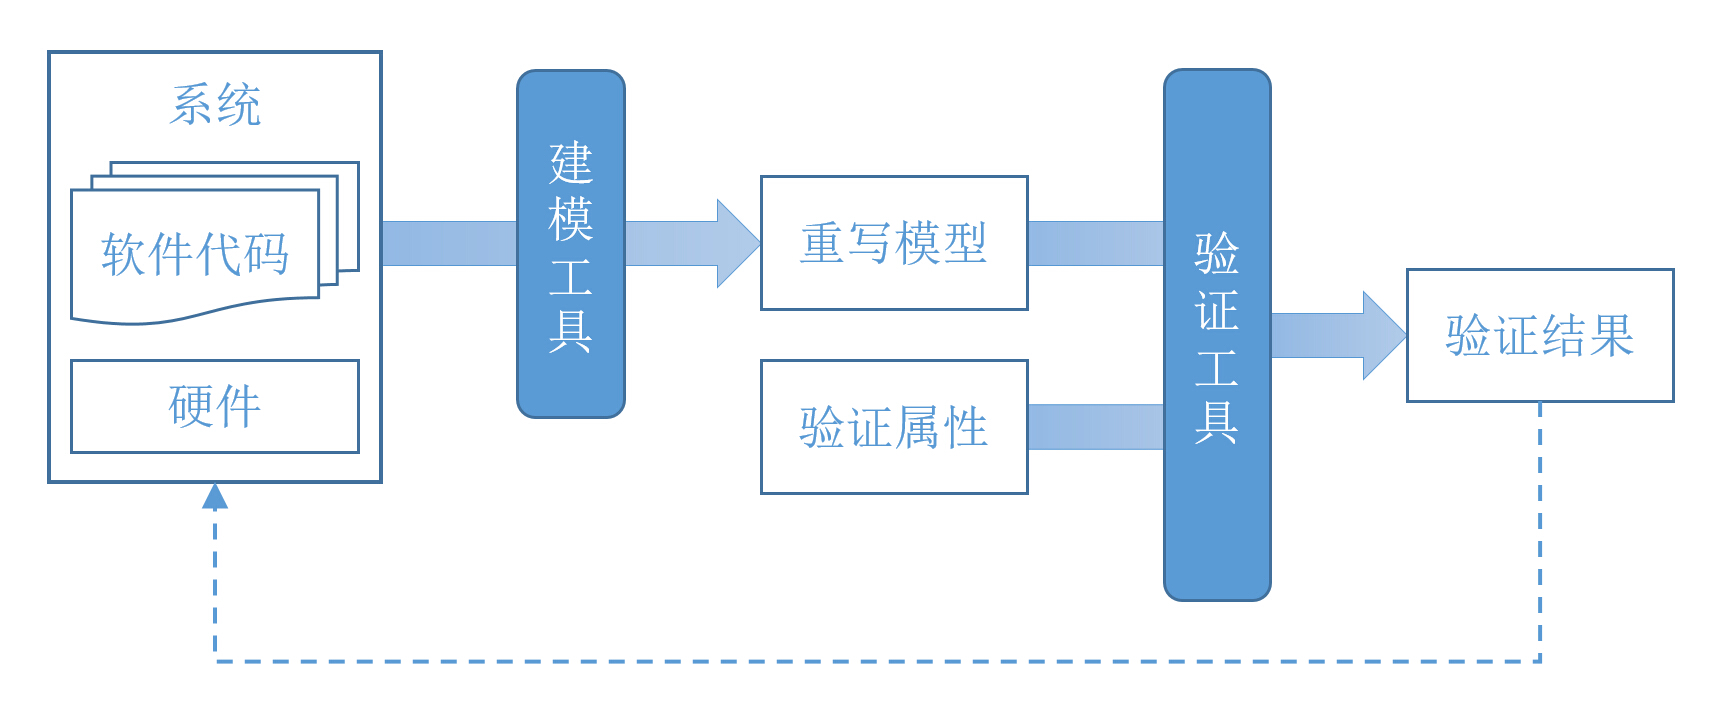
\includegraphics[width=\textwidth]{framework.jpg}
\caption{基于重写模型的形式化建模与验证流程}
\label{f:framework}
\end{figure}

在这个流程中,建模通常是一个抽象的过程。建模过程需要针对用户所关心的系统属性,对系统的某个侧面进行抽象描述。而抽象的层次,则需要建模人员根据经验进行斟酌。如果抽象层次太低,系统模型将包含大量细节,模型行为将更贴近目标系统的行为,验证结果也更有指导意义。然而模型中细节过多可能导致的后果是在验证过程中,验证工具无法处理如此大规模的模型验证。另一方面,如果抽象层次太高,虽然有利于后端验证过程的进行,但由于模型的行为描述太抽象,对应的验证结果可能对目标系统没有太多指导意义。

下面先介绍基于重写模型的系统建模思路,然后针对嵌入式系统所具有的一些特征,介绍如何利用重写模型对这些特征进行建模。

\subsection{建模框架}

\subsubsection{系统状态建模}
\label{sss:state-modeling}

对系统进行建模,首先需要对系统某一时刻的运行状态进行建模。对于基于状态的模型(比如自动机等)来说,系统的状态可以对应为模型的状态,这比较易于理解。而对于基于项表达式和规则的重写模型来说,系统状态则需要通过项表达式来进行建模。

具体地说,在基于重写模型进行系统建模时,我们通过定义函数符号来对我们所关心的系统元素(如变量、状态等)进行“编码”。通过人为地给函数符号及其每一个参数赋予语义,来给每一个项表达式赋予语义。比如在例~\ref{e:river} 中,我们规定函数符号 $\farmer$、$\wolf$、$\lamb$、$\grass$ 各自表示农夫、狼、羊、草当前所处的状态,而它们的第一个参数则表示当前该对象处于河的哪一侧。我们又规定函数符号 $\lhs$ 和 $\rhs$ 分别表示河的左岸和右岸,于是项表达式 $\farmer(\lhs) \comp \lamb(\lhs) \comp \wolf(\rhs) \comp \grass(\lhs)$ 就可以用于表示系统的某个状态,该状态为农夫在左岸、羊在左岸、狼在右岸、草在左岸。又比如在例~\ref{e:clock} 中,我们规定函数符号 $\clock$ 表示一个时钟当前的状态,而它的第一个参数表示该时钟当前的读数。而我们又给 $\s$ 和 $\zero$ 赋予了自然数的语义,于是项表达式 $\clock(\s^3(\zero))$ 就可以表示系统的某个状态,该状态的时钟读数为 3。

需要特别注意的是,项表达式可以对系统中用户自定义的数据类型进行描述。如定义~\ref{d:term} 所示,由于项表达式利用归纳方式进行定义,与函数式编程语言(如 Haskell)中数据类型的定义方式相同,因此可以对诸如结构体、链表、二叉树等自定义数据类型进行建模。

\subsubsection{系统行为建模}
\label{sss:behavior-modeling}

系统行为,可以理解为系统状态的改变方式。对于基于状态的模型来说,连接模型状态之间的变迁,就是模型状态的改变方式。因此对于这些模型来说,系统行为可以利用变迁进行建模。而对于重写模型,系统状态由项表达式来表示,因此作为定义项表达式之间变换关系的重写规则,可以用于建模系统的状态变迁,即系统行为。

具体地说,重写规则的左项表示变迁发生前的系统状态(或部分状态),规则的右项表示变迁发生后的系统状态(或部分状态),而重写规则的条件约束则定义了发生该变迁所需满足的条件。需要注意的是,由于重写规则可以包含变量符号,因此一条重写规则可以描述一种状态变迁\emph{模式},即一类状态变迁,而不仅仅是某条状态变迁。比如在例~\ref{e:river} 中,规则 $\farmer(x)\comp \lamb(x) \ra \farmer(\change(x))\comp\lamb(\change(x))$ 描述的行为是,如果当前状态为农夫和羊在河的同侧$x$,那么下一个状态,农夫和羊将会同处于河的另一侧 $\change(x)$。$x$ 可以是 $\lhs$(左岸),也可以是 $\rhs$(右岸)。又比如在例~\ref{e:clock} 中,规则 $\clock(x) \ra \clock(\add(x,\s(\zero))) \;\Dla\; \lessthan(x,\s^{11}(\zero)) = \true$ 表示,如果当前状态的时钟示数为 $x$,且满足 $x < 11$,那么下一个系统状态\emph{有可能} 为时钟示数显示 $x+1$。注意这里“有可能”的意思是,由于重写的不确定性,该状态的下一个系统状态,根据规则 $\clock(x) \ra \broken$,也有可能为 $\broken$,即表示时钟损坏。

虽然重写规则本身并不对规则两侧的项表达式作任何形式上的约束,但在利用重写模型进行系统建模时,我们通常会在两侧使用“同类型”的项表达式。这指的是,规则两侧的项表达式所建模的系统状态或元素是相同类型的。比如例~\ref{e:clock} 的规则 $\clock(x) \ra \broken$,两侧的项表达式 $\clock(x)$ 和 $\broken$ 所建模的都是系统中时钟的状态。如果存在规则 $\clock(x) \ra x$,左项表示的是时钟的状态,而右项是一个自然数,则该规则从系统行为的角度来看是不合理的。

\subsection{组件层次与并发}
\label{ss:multi-component}

一个嵌入式系统可能由若干个子模块构成,系统的功能需要由各子模块之间协作共同完成;另一方面,与通用计算机不同,嵌入式系统一般用于实现特定功能,它往往作为更上层系统的一部分,与其它嵌入式系统共存。因此,要对嵌入式系统进行建模,则要求模型本身支持组件行为的可组合性及其并发的描述。

首先需要指出,在定义~\ref{d:rewriting} 中,重写对项表达式的影响被位置 $p$ 所约束。也就是说,重写是局部进行的——当我们对某个项表达式应用重写规则进行重写时,被替换的部分不需要是整个项表达式,可以只限定于某个子项表达式。转换成系统建模的视角,这表明,通过重写规则定义的系统行为,不一定改变了整个系统状态,可以只是系统一部分的状态,即系统中某个组件的状态。

基于以上思路,多组件系统的层次结构可以利用项表达式的层次结构(定义~\ref{d:term})进行描述。假设我们用项表达式 $t_1,\ldots,t_n$ 分别对系统中 $n$ 个组件的状态进行建模,那么可以定义一个新的 $n$ 元函数符号 $f^{(n)}$,用项表达式 $f(t_1,\ldots,t_n)$ 来对整个系统状态进行建模。

至于组件行为的组合,得益于重写的局部性,定义在子项表达式上的重写规则,可以自然地应用到整个项表达式上。也就是说,子组件的行为可以在系统中独立进行。比如说,假设我们定义了重写模型 $\cR_i$ 对子组件 $i$ 的行为进行建模。那么 $\cR_i$ 的规则可以被应用于项表达式 $t_i$,表示子组件 $i$ 的状态变化。当子组件 $i$ 被置于整个系统 $f(t_1,\ldots,t_n)$ 中看待时,子组件 $i$ 的局部行为并不受影响,$\cR_i$ 的规则仍然可直接被应用于 $f(t_1,\ldots,t_n)$ 的子项表达式 $t_i$,并且不影响其它子项表达式 $t_j$($j\not=i$)。正如例~\ref{e:river},我们把农民、狼、羊和草各自看作系统中的一个子组件,整个系统的状态由函数符号“$\comp$”将各子组件连接构成。规则 $\farmer(x) \ra \farmer(\change(x))$ 实际上定义了“农民”这个子组件的行为,但它仍然可以被(局部)应用于系统状态 $\farmer(\rhs) \comp \lamb(\rhs) \comp \wolf(\lhs) \comp \grass(\lhs)$,产生新的系统状态 $\farmer(\lhs) \comp \lamb(\rhs) \comp \wolf(\lhs) \comp \grass(\lhs)$,表示农夫独自到了河对岸,而系统中其它子组件不受影响。重写技术的局部性,使组件之间的并发行为在重写模型中得到表达~\cite{DBLP:journals/tcs/Marte-OlietM02}。

\begin{figure}[ht]
\centering
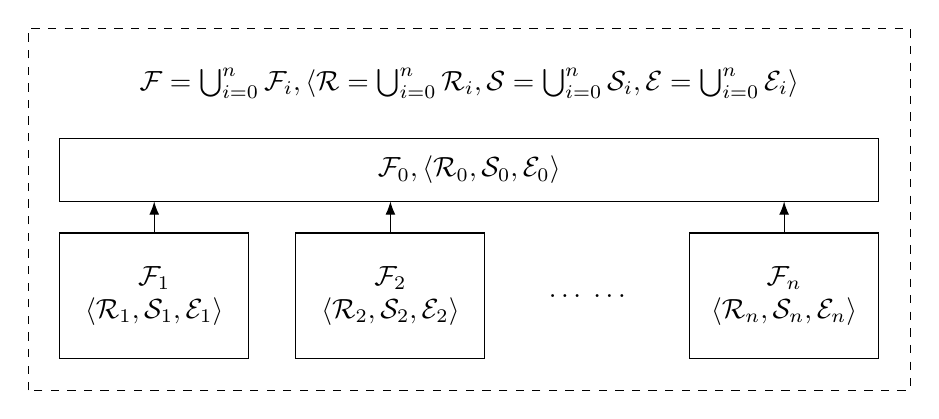
\begin{tikzpicture}
\draw (0,0) rectangle +(2.4,1.6);
\draw (1.2,0.8) node[align=center] {$\cF_1$ \\ $\lb \cR_1,\cS_1,\cE_1\rb$};
\draw [-{Latex}] (1.2,1.6) -- +(0,0.4);
\draw (3,0) rectangle +(2.4,1.6);
\draw (4.2,0.8) node[align=center] {$\cF_2$ \\ $\lb \cR_2,\cS_2,\cE_2\rb$};
\draw [-{Latex}] (4.2,1.6) -- +(0,0.4);
\draw (6.7,0.8) node[align=center] {$\ldots\;\ldots$};
\draw (8,0) rectangle +(2.4,1.6);
\draw (9.2,0.8) node[align=center] {$\cF_n$ \\ $\lb \cR_n,\cS_n,\cE_n\rb$};
\draw [-{Latex}] (9.2,1.6) -- +(0,0.4);

\draw (0,2) rectangle +(10.4,0.8);
\draw (5.2, 2.4) node [align=center] {$\cF_0, \lb\cR_0,\cS_0,\cE_0\rb$};

\draw [dashed] (-0.4,-0.4) rectangle +(11.2,4.6);
\draw (5.2, 3.5) node [align=center] {$\cF=\bigcup^n_{i=0}\cF_i, \lb \cR = \bigcup^n_{i=0}\cR_i, \cS = \bigcup^n_{i=0}\cS_i, \cE = \bigcup^n_{i=0}\cE_i \rb$};
\end{tikzpicture}
\caption{规范化条件重写模型的层次结构}
\label{f:layered-model}
\end{figure}

图~\ref{f:layered-model} 描述了当系统中存在多组件时,利用规范化条件重写模型对系统进行建模的模型层次结构。假定模型 $\lb \cR_i,\cS_i,\cE_i\rb$($1\le i\le n$)是子组件 $i$ 的行为模型。当考虑整个系统时,除了将 $\cR_i$、$\cS_i$、$\cE_i$ 直接叠加(取并集),还需要定义新的词汇表 $\cF_0$ 对系统整体状态进行建模(比如例~\ref{e:river} 的函数符号“$\comp$”),以及定义新的模型 $\lb \cR_0,\cS_0,\cE_0\rb$ 描述各组件之间的交互行为(比如同步、异步通信)。然后整个系统则可以由模型 $\lb \cR,\cS,\cE\rb$ 进行描述,其中 $\cR = \bigcup^n_{i=0}\cR_i$、$\cS = \bigcup^n_{i=0}\cS_i$、$\cE = \bigcup^n_{i=0}\cE_i$。如果系统存在更上层结构,则“递归地”进行以上建模过程。

\subsection{组件交互}

上一小节介绍了组件行为的组合建模,以及各组件局部行为之间的并发。当组件之间存在交互时,需要定义新的模型 $\lb \cR_0,\cS_0,\cE_0\rb$ 用于描述组件之间的交互行为。下面分别从同步和异步两种方式来介绍重写模型如何对组件之间的交互行为进行建模。


\subsubsection{同步}
\label{ss:sync}

组件之间的同步通信,实际上是指若干组件在满足某条件时同时发生状态改变。从重写模型的角度来说,这需要重写规则同时应用于各组件对应的子项表达式。因此,描述同步行为的重写规则应该定义在描述整个系统的项表达式上,即包含 $f\in\cF_0$ 的项表达式。该规则的左项不应该仅仅包含某个子组件对应的子项表达式,而应该包含该同步行为涉及的所有组件对应的多个子项表达式。比如在例~\ref{e:river} 中,重写规则 $\farmer(x)\comp \wolf(x) \ra \farmer(\change(x))\comp\wolf(\change(x))$ 是一条描述同步行为的规则。规则的左项包含了组件“农民”和“狼”,只有满足农民和狼的位置相同(都为 $x$)这一条件,该同步行为才能发生。产生的状态变化是:农民和狼同时来到了 $x$ 的另一侧 $\change(x)$。

举个例子,比如我们希望描述一个具有两个时钟的系统,我们定义二元函数符号 $f^{(2)}$ 来建模整个系统的状态,它的两个参数都是例~\ref{e:clock} 中定义的 $\clock$,分别代表两个时钟当前的状态。因此 $f(\clock(\zero),\clock(\s(\zero)))$ 表示当前系统状态为:时钟1的示数为 0,时钟 2 的示数为 1。如果我们希望两个时钟同步运行,那么我们不能使用例~\ref{e:clock} 中给单个时钟定义的重写规则,它们会产生重写序列:
\begin{eqnarray}
 f(\clock(\s^0(\zero)),\clock(\s^0(\zero)))  
 & \ra & f(\clock(\s^1(\zero)),\clock(\s^0(\zero))) \nonumber \\
 & \lrps{}{} & f(\clock(\s^2(\zero)),\clock(\s^0(\zero))) \nonumber \\
 & \lrps{}{} & f(\clock(\s^2(\zero)),\clock(\s^1(\zero))) \mbox{。} \nonumber
\end{eqnarray}
以上序列表明两个时钟是各自并发运行的,之间没有任何关系。我们需要定义以下同步规则\footnote{注意这里为了方便理解,该规则省略了应满足的约束条件 $x<11$。}
\begin{eqnarray}
 f(\clock(x),\clock(x)) & \ra & 
 f(\clock(\add(x,\s^1(\zero))),\clock(\add(x,\s^1(\zero)))) \nonumber
 \end{eqnarray}
描述满足我们需求的同步行为:当系统中的两个时钟示数相同(都为 $x$)时,两个时钟的示数同时加 1。于是有以下重写序列,描述了系统中两个时钟同步运行:
\begin{eqnarray}
 f(\clock(\s^0(\zero)),\clock(\s^0(\zero)))  
 & \ra & f(\clock(\s^1(\zero)),\clock(\s^1(\zero))) \nonumber \\
 & \lrps{}{} & f(\clock(\s^2(\zero)),\clock(\s^2(\zero))) \nonumber \\
 & \lrps{}{} & f(\clock(\s^3(\zero)),\clock(\s^3(\zero))) \mbox{。} \nonumber
\end{eqnarray}

\subsubsection{异步}
\label{ss:async}

异步事件触发的行为可以抽象地拆解成两个行为:组件 1 触发事件 A,事件 A 使组件 2 的状态发生变化。如果将事件 A 看作系统中的一个子组件,则这两个行为可以分别看作两个同步行为。在对异步行为进行建模时,我们采取这种方式把异步行为拆解成两个同步行为进行建模。

下面举个例子说明。假设组件 1 的状态可以从 $a$ 变成 $b$,从 $b$ 变成 $c$,从 $c$ 变成 $d$;当它从状态 $b$ 变成状态 $c$ 时,同时会给系统中的组件 2 发送一个消息 $m$。假设组件 2 在状态 $e$ 会等待从组件 1 发送过来的消息 $m$;收到消息后状态会变成 $g$。那么我们将组件 1 和组件 2 之间用于传输消息 $m$ 的信道也作为系统的一个组件进行考虑。定义三元函数符号 $f^{(3)}$ 用于建模系统状态,它的第一个参数表示组件 1 的状态,第二个参数表示信道的状态,第三个参数表示组件 2 的状态。于是我们可以用以下规则来对上述异步行为进行描述:
\begin{eqnarray}
 a & \ra_1 & b \nonumber \\
 f(b,x,y) & \ra_2 & f(c,m,y) \nonumber \\
 c & \ra_3 & d \nonumber \\
 f(x,m,e) & \ra_4 & f(x,\myempty,g) \;\mbox{,} \nonumber
\end{eqnarray}
其中常数 $\myempty$ 表示信道中无消息。 规则 2 是组件 1 和信道组件的同步行为,它表示“组件 1 的状态从 $b$ 变成 $c$”这个动作必须和“信道中有消息 $m$ 出现”这个动作同时发生,且注意该同步行为不涉及组件 2——其状态 $y$ 不发生改变。而规则 4 则是信道组件和组件 2 的同步行为,它表示“信道中的消息 $m$ 消失”这个动作必须与“组件 2 的状态从 $e$ 变成 $g$”这个动作同时发生。规则 2 和规则 4 是典型的异步行为建模规则。由上述规则可以产生如下重写序列:
\begin{eqnarray}
& & f(a,\myempty,e)  \ra  f(b,\myempty,e) 
  \ra f(c,m,e) \ra f(d,m,e)  \ra f(d,\myempty,g) \;\mbox{。} \nonumber
\end{eqnarray}
该序列表明,组件 1 向组件 2 发出消息 $m$ 后,不需等待组件 2 的响应,即可继续运行(从状态 $c$ 变成状态 $d$)。需要注意的是,状态 $b$ 与 $g$ 可以进一步细化为与消息 $m$ 有关的项表达式,如 $b=b'(m)$、$g=g'(m)$,表示组件 1 向组件 2 传递信息。 


\subsection{软硬件行为}
\label{ss:hw-sw}

嵌入式系统通常由软硬件混合构成,而软件与硬件的行为差异在于,硬件行为通常具有并发性,而软件代码通常以顺序方式执行。从建模的角度对组件的顺序行为与并行行为进行考虑,它们可以进一步被抽象成两类行为——确定性行为与不确定性行为,分别对应于规范化条件重写模型 $\RSE$ 的规则集 $\cS$ 与 $\cR$。

对组件的局部行为,若是顺序执行的(例如不涉及共享变量访问的软件代码),则将其建模为局部确定性行为,即建模为 $\cS_i$ 的重写规则;若该行为具有不确定性(例如硬件模块随时可能发生物理失效),则将其建模为局部不确定性行为,即通过 $\cR_i$ 的重写规则进行建模。对组件间的交互行为,考虑到它可能对系统中其它行为产生影响(例如对共享变量进行写操作可能影响其它线程对该变量的读操作),因此将其建模为全局的不确定性行为,即描述为 $\cR_0$ 的重写规则。

\begin{figure}[ht]
\centering
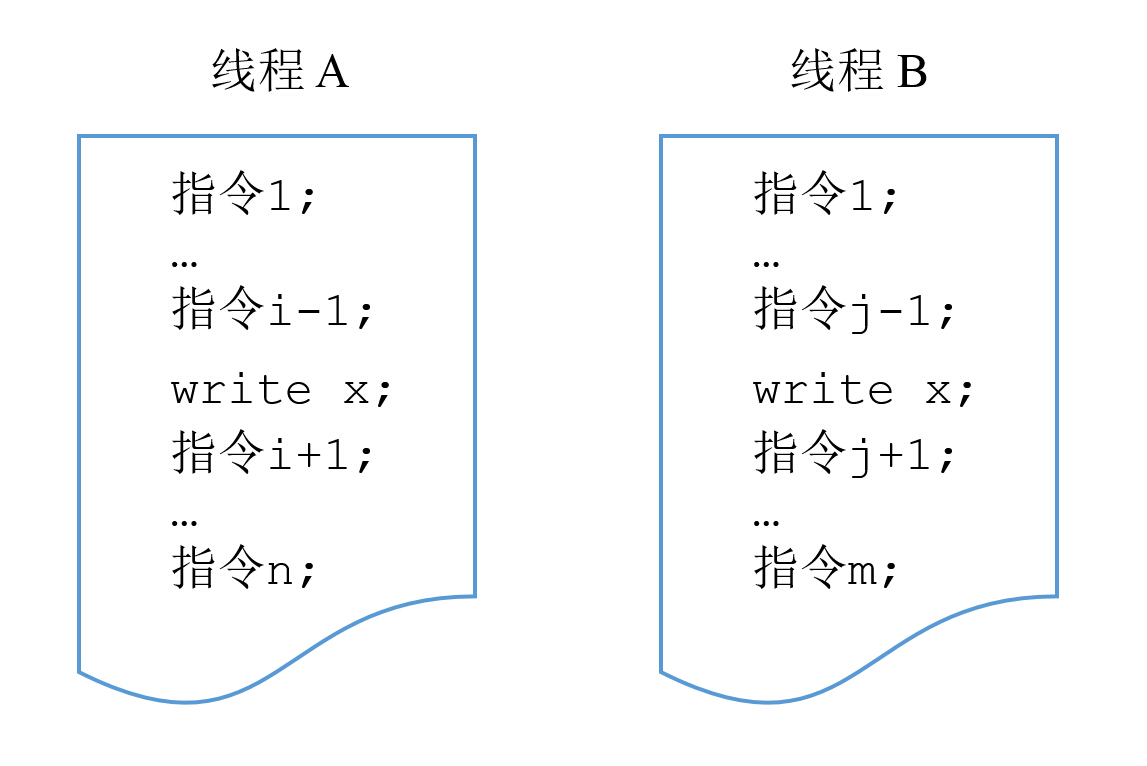
\includegraphics[width=0.7\textwidth]{concur.jpg}
\caption{两个线程的并发}
\label{f:concur}
\end{figure}

如图~\ref{f:concur} 的例子,假设变量 x 是全局变量,线程 A 的指令 i 和线程 B 的指令 j 都对 x 进行写操作,因此这两条指令被调度运行的先后次序将对整个系统的运行结果产生影响,它们应当被建模成 $\cR_0$ 中的全局不确定性规则。假设线程 A 的其它指令以及线程 B 的其它指令都与变量 x 无关,虽然这些指令相互之间并发运行,但实际上系统对这些指令的调度并不会影响运行结果,因此它们可被建模成 $\cS_i$ 的局部确定性规则。

从模型组合的角度来看,不同组件的局部确定性行为 $\cS_i$ 作用于项表达式的不同位置,因此这些行为组合得到的系统行为模型 $\cS$ 具有终止性与合流性~\cite{DBLP:journals/jacm/Huet80},满足规范化条件重写模型 $\RSE$ 的要求。

根据规范化重写的定义(定义~\ref{d:normalrewriting}),$\cS$ 规则的应用是附属于 $\cR$ 规则的,以上建模策略让系统中行为的重要程度在规范化重写模型中有所体现。另一方面,根据定义~\ref{d:normalrewriting},应用 $\cR$ 规则前后都需要对整个项表达式应用 $\cS$ 规则进行规范化,这就保证了规范化重写序列与系统状态变迁路径的对应性。同时,在这一建模策略下,由于 $\cS$ 规则对应的行为被“嵌入”到 $\cR$ 规则对应的行为中,相当于若干行为被抽象成单一行为,这使得系统的状态空间数得以减少\footnote{这意味着被抽象的中间状态必须与验证属性无关。},为后端的验证过程提供了便利。


\subsection{组件的动态结构}
\label{ss:dynamic-component}

在嵌入式系统中,存在组件结构的动态行为。比如在事件响应系统中,接收到一个事件请求后,系统可能创建一个新线程对该事件进行处理;又比如在无线传感网络中,因为主观连接需求或者客观的通信信号问题,网络中的节点拓扑通常会产生变化。这些行为都涉及到组件结构的改变。
这就对建模模型提出了两个问题:如何对这种组件结构变化进行建模?如何对新增的组件行为进行建模?

首先是对组件结构变化的建模方式。由于项表达式描述的不仅仅是系统中某些变量的状态,而是整个系统的状态,其中包括系统的结构信息。在第~\ref{ss:multi-component} 小节中提到,系统组件的数量由函数符号的元数进行描述。如果系统中组件数量可变,那么我们需要函数符号的元数可变——这违背了词汇表 $\cF$ 的定义。然而,得益于规范化重写模型丰富的表达能力,我们可以利用等价模型 $\cE$ 来模拟元数可变的函数符号。实际上,解决思路早已在例~\ref{e:river} 中给出——定义二元(中缀)函数符号“$\comp$”。如果它具有结合律,即以下等价规则属于 $\cE$,
\begin{eqnarray}
 (x\comp y) \comp z & \sim & x \comp (y\comp z)\;\; , \nonumber
\end{eqnarray}
那么由“$\comp$”构成的项表达式中的括号可以省略。它定义了一个列表结构,列表中的元素数量可变。例如 $a\comp b$、$a\comp b\comp c\comp d$、$a\comp b\comp c\comp d\comp e$ 都是列表。如果函数符号“$\comp$”同时还具有交换律,即以下等价规则属于 $\cE$,
\begin{eqnarray}
 x\comp y & \sim & y\comp x\;\; , \nonumber
\end{eqnarray}
那么由“$\comp$”构成的项表达式中,不仅括号可以省略,而且元素之间的顺序变得无关重要。它定义了一个多重集合结构,多重集合中的元素数量可变,且元素无序。例如 $a\comp a\comp c\comp d$ 和 $a\comp d\comp c\comp a$ 都是多重集合,且 $(a\comp a\comp c\comp d) =_{\cE} (a\comp d\comp c\comp a)$。下面假设“$\comp$”同时具有交换律和结合律。

基于这种结构可变的模型,改变结构的行为可以被建模成对应的改变项表达式结构的重写规则。例如要描述以下行为:线程 $f$ 在状态 $a$ 创建一个新线程 $g$,$g$ 的初始状态为 $a'$,而线程 $f$ 在创建 $g$ 以后进入状态 $b$。那么我们可以用以下重写规则:
\begin{eqnarray}
f(a) & \ra & f(b) \comp g(a') \nonumber
\end{eqnarray}
来描述线程 $g$ 的创建过程。又比如在例~\ref{e:river} 中,我们可以用以下规则:
\begin{eqnarray}
\wolf(x)\comp\lamb(x) & \ra & \wolf(x) \nonumber
\end{eqnarray}
描述狼把在同侧的羊吃掉的行为。这也是一种系统组件结构发生变化的行为。

在对“产生新组件”这一行为进行建模后,还需要对新组件本身的行为进行建模。由于新组件的行为是可预知的(比如处理某类事件的方式),因此描述新组件行为的重写规则只需如其它行为一样,定义在规则集 $\cS$ 或 $\cR$ 中即可。

在这里我们可以看到基于重写模型建模的一大优点:基于项表达式的状态建模,可以描述系统结构的变化,使建模人员不需要对动态产生的新组件数量上限进行假设。

\subsection{实时性}
\label{ss:realtime-modeling}

许多嵌入式系统的正确性不仅要求满足逻辑正确性,还需要满足某些时间约束,这类系统称之为\emph{实时系统}。对于实时系统的建模,要求模型中支持对“时间”的建模。针对重写模型,我们在系统的项表达式中,增加一个用于描述时间的子项表达式,例如项表达式
\begin{eqnarray}
& & f(t_1,\ldots,t_n,\; time) \nonumber
\end{eqnarray}
中,$f^{(n+1)}$ 的最后一个参数。而位于 $time$ 位置的子项表达式可以采用自然数集(如例~\ref{e:nat})表示离散的时间,也可以采用非负实数集~\cite{DBLP:journals/tcs/GoguenM92} 表示连续的时间,这取决于建模人员对模型精确度的要求,也取决于验证工具的验证能力。

需要注意的是,由于我们将“时间”作为组件在模型中进行描述,因此系统中所有需要耗时的行为都将被建模成同步行为,需要与“时间”组件进行同步。例如下列规则:
\begin{eqnarray}
f(a,\; x_{time}) & \ra & f(b,\; x_{time}+1) \nonumber
\end{eqnarray}
描述了系统从状态 $a$ 变成状态 $b$ 的行为,这一行为需要耗时 1 个时间单位。

\section{支持工具集}
\label{s:tool}

本小节将基于语义映射的方式,将上述建模框架在工具集 Maude 中予以实现。

\subsection{Maude}

\emph{Maude}~\cite{DBLP:journals/tcs/ClavelDELMMQ02} 是一种基于重写逻辑~\cite{DBLP:journals/jlp/Meseguer12} 的语言和工具,它能支持形式化建模和对模型的分析验证。

\subsubsection{建模}
Maude 将系统建模成为\emph{模块}(module)。一个模块相当于一个\emph{重写逻辑模型}(rewrite theory) 
$\mathcal{R^L} = \lb\Sigma,\mathit{A},\mathit{E} , \mathit{R}\rb$,其中:
\begin{itemize}
\item $\Sigma$ 是一个带类型的词汇表。它包括函数符号、\emph{类型}\footnote{注意这里应指\emph{类别},与“类型”有所区别。为了便于读者理解,本文称之为“类型”。}(sort)和\emph{子类型}(subsort)的声明。 函数符号允许使用中缀记法、前缀记法、后缀记法或混合记法,利用下划线“\verb|_|” 表示参数的位置。项表达式的定义与重写模型相同。
\item $\lb\Sigma, \mathit{E}\cup\mathit{A}\rb$ 是一个\emph{带成员关系的等词逻辑理论}~\cite{DBLP:journals/tcs/BouhoulaJM00}(membership equational logic theory)。其中,$\mathit{E}$ 是条件等式(conditional equation)和成员关系规则的集合,
$\mathit{A}$ 是一个性质集合,比如交换律、结合律等。
\item $\mathit{R}$ 是一个\emph{带标签的条件重写规则} 集合。它描述了系统的单步状态变迁。每一条规则的形式为 $[l]~:~t\rightarrow t'\mbox{ \textbf{if}
  }\bigwedge^n_{j=1}cond_j$,其中 $cond_j$ 是形如 $u_j=v_j$ 的约束条件,$l$ 是该规则的标签,$t,t',u_j,v_j$ 都是项表达式。该规则的语义与条件重写规则(定义~\ref{d:crule})的语义相同。
\end{itemize}

Maude 还支持面向对象风格的建模。类声明
\begin{eqnarray}
& & \texttt{class }C\texttt{ |
}att_1\texttt{:}s_1\texttt{,}\ldots\texttt{,}att_n\texttt{:}s_n \nonumber
\end{eqnarray}
定义了一个新类,类名为 $C$,它包含类属性 $att_1,\ldots,att_n$,它们分别具有类型 $s_1,\ldots,s_n$。类 $C$ 的一个\emph{对象}(或称“\emph{实例}”)表示为项表达式
\begin{eqnarray}
\texttt{< } O\texttt{:} C \texttt{ | }
att_1\texttt{:}val_1\texttt{,} \ldots
\texttt{,}att_n\texttt{:}val_n\texttt{ >} \;\mbox{。} \nonumber
\end{eqnarray}
其中,$O$ 是该对象的\emph{标识}(identifier),具有类型 \verb|Oid|;
$val_i$ 是属性 $att_i$ 的值。所有类的对象都具有类型 \verb|Object|。重写规则可以针对某个类的项表达式进行定义。\emph{子类}(subclass)可以继承其父类的所有类属性以及相关的重写规则。

\emph{Real-Time Maude}~\cite{DBLP:journals/lisp/OlveczkyM07} 是 Maude 的一个扩展,它同时给 Maude 语言和工具集增加了新功能。它主要的目的是让 Maude 可以支持实时系统的建模和分析验证。在Maude的基础上,Real-Time Maude 内置了一个名为“\verb|Time|”的描述时间的模块。在 Maude 模块的基础上,Real-Time Maude 在集合 $\mathit{R}$ 中加入了\emph{带标签的单元计时规则}(labeled tick rule)。单元计时规则具有以下形式
\begin{eqnarray}
& & [l]~:~\{s\}\rightarrow\{s'\} \mbox{\textbf{ in time}
  }r\mbox{ \textbf{if} }cond \;\; , \nonumber
\end{eqnarray} 
用于描述系统的时间行为。它表示当条件 $cond$ 满足时,系统从状态 $s$ 变成目标状态 $s'$,(全局)时间往前推移 $r$ 个时间单位。为了区别于单元计时规则,$\mathit{R}$ 中原来的不涉及时间的重写规则,称作\emph{瞬时规则}(instantaneous rule),应用该规则时(全局)时间保持不变。

需要注意的是,Maude 面向对象风格的模型以及其扩展 Real-Time Maude 都只是一种语法封装,它们的底层仍基于重写逻辑模型 $\mathcal{R^L}$ 和重写逻辑。 

\subsubsection{模型分析及形式化验证}
给定一个重写逻辑模型,Maude 和 Real-Time Maude 给用户提供了许多配套工具对模型进行分析。例如,\verb|rewrite| 指令可以符号化地、抽象地执行目标模型,在模型的层次上对系统进行仿真;给定一个初始状态(用项表达式表示),\verb|search| 指令可以搜索所有可达的状态,从中判断是否存在满足指定性质的状态;Maude 配套的\emph{交互式定理证明器}~\cite{DBLP:journals/jucs/ClavelPR06}(Inductive Theorem Prover,ITP)可以通过交互式的方法,用于证明模型具有的等词逻辑性质。

在本文中,我们更关心的是 Real-Time Maude 配套的形式化验证工具——\emph{LTL 模型检测器}~\cite{DBLP:journals/entcs/EkerMS02}(LTL model checker)。它可以检查是否模型中的\emph{任意} 一条行为路径都满足给定的时序逻辑公式。\emph{状态命题}(state proposition)被定义为具有类型 \verb|Prop| 的项表达式。它们的语义由集合 $\mathit{E}$ 中以下形式的条件等式进行规定:
\begin{eqnarray}
\texttt{ceq
} \mathit{statePattern} \texttt{ |= } \mathit{prop} \texttt{ = } b
\texttt{ if } cond\;\; , \nonumber
\end{eqnarray}
其中,$b$ 是具有类型 \verb|Bool| 的项表达式。该条件等式表示,当 $cond$ 成立且当前状态的项表达式是 $\mathit{statePattern}$ 的实例时, $\mathit{prop}$ 的值等于 $b$。所有这种形式的条件等式共同定义了命题 $\mathit{prop}$ 成立的条件:命题 $\mathit{prop}$ 在状态 $s$ 成立,当且仅当 $s$ 满足 $s \texttt{ |= } \mathit{prop}$ 等于 \verb|true|。\emph{时序逻辑公式}~\cite{DBLP:books/daglib/0077033}(temporal logic formula)由状态命题和时序逻辑操作符(operator)构成。时序逻辑操作符包括但不限于 \verb|~|(非)、\verb|\/|(或)、\verb|[]|(“总是”)、\verb|<>|(“最终”)、\verb|U|(“直到”)。 Real-Time Maude 支持\emph{时控的}(timed)和\emph{非时控的}(untimed)LTL 模型检测。本文的案例将会用到非时控的 LTL 模型检测命令
\begin{eqnarray}
  \texttt{(mc } s \texttt{ |=u } \Phi \texttt{ .)} \nonumber
\end{eqnarray}
该命令检查的是,给定初始状态 $s$,从 $s$ 开始的所有行为序列是否\emph{在所有时刻} 都满足时序逻辑公式 $\Phi$。


\subsection{建模框架实现} 
\label{ss:method-impl}

如果将重写逻辑模型 $\mathcal{R^L} = \lb \Sigma, A, E, R\rb$ 的 $\Sigma$、$A$、$E$、$R$ 分别与规范化条件重写模型 $\RSE = \lb \cR,\cS,\cE\rb$ 的 $\cF$、$\cE$、$\cS$、$\cR$ 对应起来,两者存在许多相似之处,然而它们的主要区别在于:
\begin{enumerate}[(i)]
\item 重写逻辑模型 $\mathcal{R^L}$ 的性质集合 $A$ 只支持交换律、结合律、单位元性质(identity)和幂等性(idempotency),而规范化条件重写模型 $\RSE$ 的等价模型 $\cE$ 支持一般化的等式规则,覆盖了 $A$ 的支持范围;
\item 重写逻辑模型 $\mathcal{R^L}$ 的重写过程基于类重写~\cite{lankford77b},即重写规则应用的对象是项表达式关于 $E$ 的等价类,而规范化条件重写(定义~\ref{d:cnormalrewriting})基于规范化过程,即重写规则应用的对象是项表达式关于 $\cS$ 的范式;
\item 重写逻辑模型 $\mathcal{R^L}$ 带类型信息,而规范化条件重写模型 $\RSE$ 不带类型信息。
\end{enumerate}

区别 (ii) 是两者在理论模型上的区别。然而,Clavel 等人在文献~\inlinecite{DBLP:journals/tcs/ClavelDELMMQ02} 中指出,Maude 在具体实现时,为了保证工具效率,采取了与规范化重写相似的重写策略。
%——将 $E$ 中的条件等式看作有向规则,并利用 $E$ 对项表达式进行规范化。

\begin{algorithm}[ht] 
    \KwIn{规范化条件重写模型四元组 $\cF$, $\cE$, $\cS$, $\cR$}
    \KwOut{重写逻辑模型四元组 $\Sigma$, $A$, $E$, $R$}

    $\Sigma = \cF$\;
    $R = \cR$\;
    $A = \emptyset$\;

    \ForEach{$e \in \cE$}{
        \If{$e$ 表示交换律、结合律、单位元性质或幂等性}{
            $A = A \cup \{e\}$\;    
        }
    }

    $\cE' = \cE \setminus A$\;
    bool $exist = false$\;

    \tcp{$directed(\cE')$ 计算 $\cE'$ 中等式有向化产生的所有可能的重写规则集}
    \ForEach{$\vec{\cE'} \in directed(\cE')$}{
        \If{模重写模型 $(\vec{\cE'}\cup\cS)_A$ 是终止且合流的 }{
            $exist = true$\;
            break \;    
        }
    }

    \uIf{ $exist = true$ }{
        $E = \vec{\cE'} \cup \cS$\;
    } \Else {
        转换失败\;
    }
\caption{规范化条件重写模型转换成重写逻辑模型}
\label{alg:convert}
\end{algorithm}

因此,本文提出算法~\ref{alg:convert},将(部分)规范化条件重写模型转换为重写逻辑模型。转换的关键点在于:重写逻辑模型的集合 $A$ 所支持的(等式)性质不及规范化条件重写模型的集合 $\cE$ 一般化,因此对于 $\cE$ 中不被支持的等式规则,需要将其有向化,转换成重写规则放入集合 $E$。所以该算法转换成功与否的关键,就在于有向化后的规则集 $\vec{\cE'}$ 能否满足重写逻辑对集合 $E$ 的要求,即必须是终止且合流的。

基于算法~\ref{alg:convert},我们将第~\ref{s:modeling} 小节提出的建模方法在 Maude 中予以实现,并通过两个真实应用案例(第~\ref{s:TO} 小节和第~\ref{s:RMS} 小节),验证它的可行性。 



\section{应用案例:铁路机车节能优化控制系统}
\label{s:TO}

铁路机车节能优化控制系统~\cite{DBLP:journals/tc/HuangDYS16}(以下简称“优化控制系统”)是由清华大学软件学院智能交通实验室与中车信息技术有限公司合作开发的一套铁路机车智能巡航控制与节能产品,用以辅助司机通过自动控制机车来最大限度降低机车的能耗。该系统对机车进行控制的过程中涉及到自动控制与司机手动控制状态的转换。本小节基于第~\ref{s:modeling} 小节提出的建模方法,利用 Maude 工具对该系统的状态转换逻辑进行建模和形式化验证。通过建模过程和验证方法的应用,我们定位了系统中的若干缺陷,并与开发人员进行了确认,帮助开发人员进行修复。

\subsection{背景介绍}

\begin{figure}[ht]
\centering
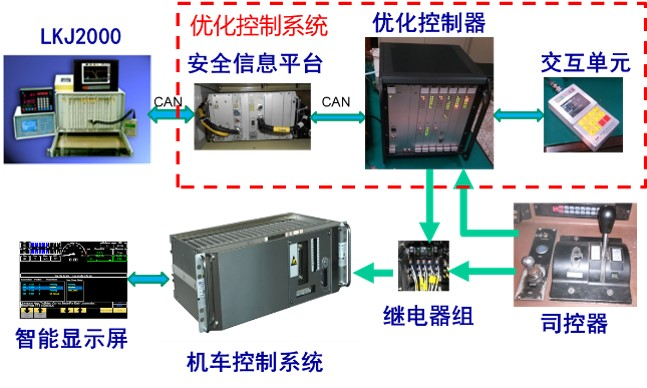
\includegraphics[width=\textwidth]{TO-system.jpg}
\caption{铁路机车节能优化控制系统}
\label{f:TO-system}
\end{figure}

优化控制系统的组成及其涉及到的周边部件如图~\ref{f:TO-system} 所示。LKJ2000 负责向优化控制系统提供铁路线路信息以及实时信息(如信号灯、是否限速等)。在手动控制状态下,机车驾驶员通过司控器进行机车的档位控制。继电器组和机车控制系统对机车进行物理控制。智能显示屏显示机车的实时状态。而优化控制系统本身主要由三部分构成。安全信息平台负责处理从 LKJ2000 接收的数据,向优化控制器提供必要的数据。优化控制器是整个系统的核心,负责列车控制逻辑和控制策略的计算。交互单元则是驾驶员与优化控制器的交互媒介。

机车在运行过程中分为自动控制和手动控制两种状态。机车自动控制时,优化控制器基于离线计算的控制策略,结合在线根据机车状态、线路信息和实时信息计算得到的调整策略,对机车进行控制。当机车处于手动控制状态时,由驾驶员通过司控器对机车进行控制。自动控制状态和手动控制状态之间的转换,可以由驾驶员主动发起,也可能由于机车的状态或铁路的实时信息满足一定条件,从而触发自动和手动控制状态的转换。

机车控制状态的转换由优化控制器负责完成。优化控制器综合从安全信息平台接收的数据、从交互单元获取的操作数据、以及司控器的档位数据,根据业务逻辑计算当前的控制策略(包括是否自动控制、控制档位等)。控制状态转换的逻辑基于事件处理机制。也就是说,优化控制器把安全信息平台向其发送的数据到达看作一个事件,把驾驶员通过交互单元进行的操作也看作一个事件,驾驶员通过司控器调整档位也被当作一个事件。优化控制器对这些外部事件进行处理,产生一个事件(数据帧)发送给继电器组,通知继电器组当前应采取的控制状态及控制档位。图~\ref{f:auto2manual} 是一个从自动控制状态转换成手动控制状态的流程示例。

\begin{figure}[ht]
\centering
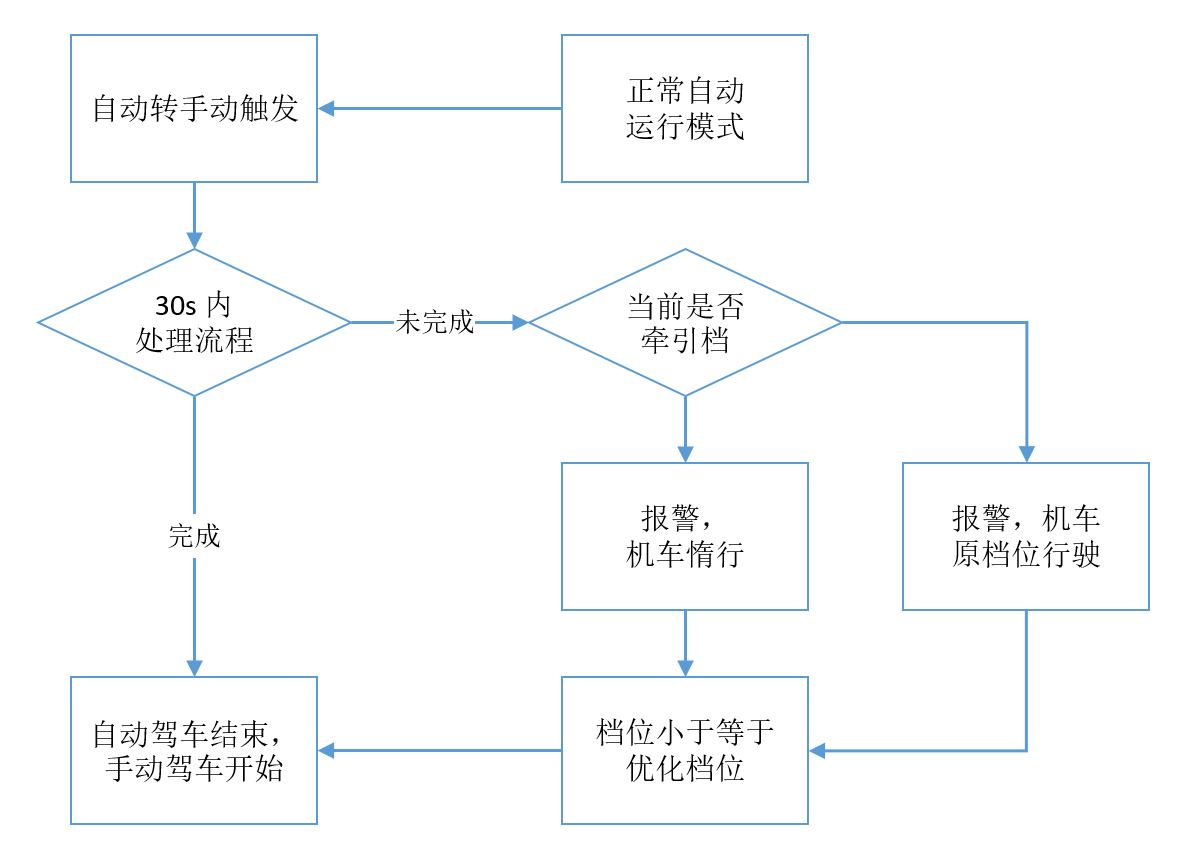
\includegraphics[width=0.9\textwidth]{auto2manual.jpg}
\caption{自动控制到手动控制的转换流程示例}
\label{f:auto2manual}
\end{figure}

优化控制器内部由若干独立模块组成,各模块拥有独立的处理器,且以多线程的方式工作。模块之间的交互也通过事件处理机制完成。因此整个优化控制器,乃至整个优化控制系统,是一个高度并发的分布式系统。系统是否对每一个事件都进行了正确的响应,事件处理的正确性是否受到并发影响,是开发人员及用户迫切关心的问题。本小节主要关心涉及机车控制状态转换的事件处理。


\subsection{系统描述}

\begin{figure}
\centering
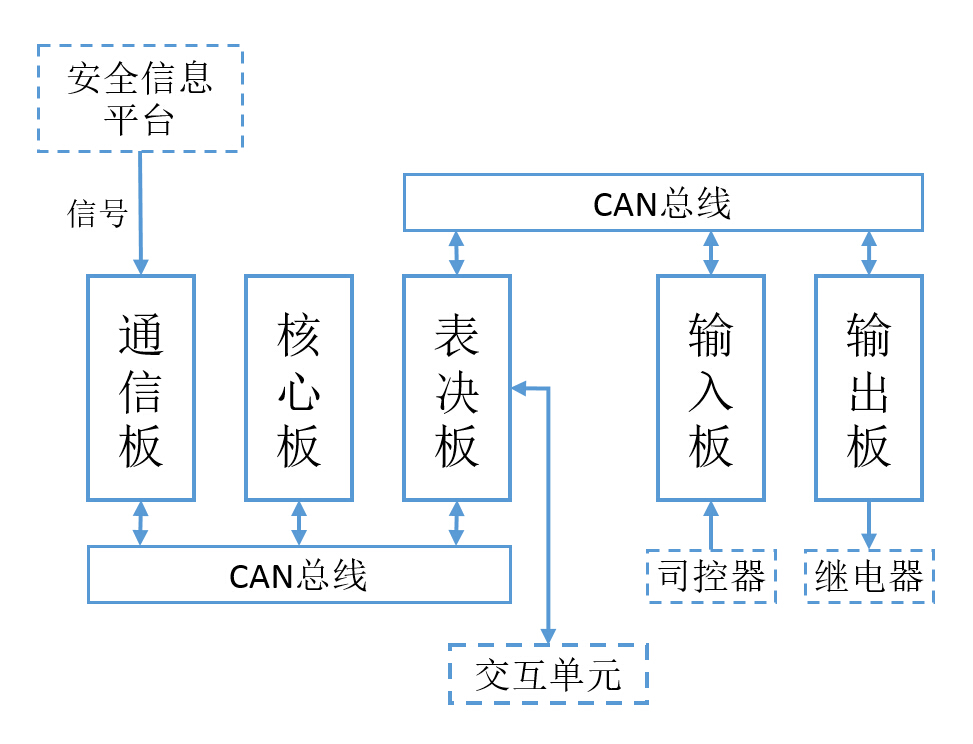
\includegraphics[width=0.7\textwidth]{TO-module.jpg}
\caption{优化控制器内部结构}
\label{f:TO-module}
\end{figure}

优化控制器的内部结构如图~\ref{f:TO-module} 所示,主要由通信板、核心板、表决板、输入输出板以及连接各板卡的总线组成。输入板的功能是将司控器的档位信息发送给表决板。输出板的功能是将表决板的计算结果(控制状态和档位信息)发送到继电器。通信板从安全信息平台接收线路信息以及实时信息,经处理后转发到核心板。核心板接收来自通信板的线路信息和实时信息,根据优化算法计算优化控制策略。然后核心板将优化计算结果发送至表决板。表决板综合考虑来自核心板的优化控制策略、通过交互单元获得的用户操作信息、以及来自输入板的档位信息,根据业务逻辑产生机车的控制策略(自动或手动控制、档位信息等),发送到输出板。

每一块板卡都维护了一个线程池,板卡的每一个端口都有一个单独的线程负责监听。当有新消息帧到来时,负责监听的线程根据该消息帧的类型,创建一个新线程对其进行处理,然后该监听线程继续监听端口消息。被创建的新线程根据自身业务逻辑对该消息帧进行相应的操作,对其计算、转发、触发一个业务流程、或再创建另一个线程等,执行完毕后线程释放。板卡的业务逻辑由多个线程协作共同完成。线程的调度由板上的操作系统完成。


\subsection{系统建模}

我们验证的对象是优化控制系统中涉及控制状态转换的事件处理机制,即相关线程的创建、计算、转发消息等行为,因此我们选择将优化控制系统中的通信板、核心板、表决板、输入输出板以及连接各板卡之间的总线进行建模,并且为安全信息平台和交互单元建立简单的模型,描述它们与优化控制器之间的交互。

对该系统建模的难点在于:
\begin{enumerate}  
\item 对复杂的数据结构及其存储进行建模。系统由 C 语言实现,代码量巨大,涉及的数据类型复杂,频繁使用各种结构体类型。这要求对数据类型进行建模,且对相应的存储结构(内存)也进行建模。
\item 对板卡间的通信进行建模。
\item 对线程调度进行建模。线程调度由板载操作系统负责,在建模过程中需要考虑线程调度的影响。
\item 对线程以及线程的创建释放进行建模。线程的行为是该系统进行事件处理及实现业务逻辑的关键行为,需要对其进行较准确的刻画。
\end{enumerate}

下面就以上关键点,结合第~\ref{s:modeling} 小节提出的建模方法与第~\ref{ss:method-impl} 小节定义的规范化条件重写模型与 Maude 模型之间的语义映射,对该系统的建模过程进行介绍。

\subsubsection{复杂数据类型及内存}

在第~\ref{sss:state-modeling} 小节已经提到,得益于项表达式的归纳结构,我们可以利用它定义非常复杂的数据类型。同时又得益于 Maude 语言提供的灵活语法,复杂数据结构得以直观地表示。例如我们用 Maude 类型 \verb|RtCore| 对 C 结构体类型 RtCore 进行建模, \verb|RtCore| 的定义如下:
\begin{verbatim}
  sort RtCore .
  op `(rt-gear:_`,rt-enable-status:_`) 
       : Nat Nat -> RtCore [ctor] .
\end{verbatim}
第 1 行用 \verb|sort| 关键字声明了一种新类型。其余两行用 \verb|op| 关键字声明了一个新的函数符号 \verb|(rt-gear:_,rt-enable-status:_)|,它的两个参数分别为 \verb|Nat|(自然数)类型和 \verb|Nat| 类型,返回类型为 \verb|RtCore|。两个下划线“\verb|_|”的位置为该函数符号的两个参数位置。于是项表达式 \verb|(rt-gear:3,rt-enable-status:0)| 表示一个类型为 \verb|RtCore| 的结构体数据,它的 rt-gear 域为 3,rt-enable-status 域为 0。

结构体类型也可以进行嵌套,比如以下表示结构体类型 RtVote 的类型 \verb|RtVote|:
\begin{verbatim}
  sort RtVote .
  op `(rt-core:_`,rt-control-status:_`) 
       : RtCore ControlStatus -> RtVote [ctor] .
\end{verbatim}
它的第一个参数类型为 \verb|RtCore|,是一个表示结构体的项表达式类型。

除了结构体,其它复合类型如第~\ref{ss:dynamic-component} 小节提到的列表和多重集,都可以在 Maude 中进行建模。

针对内存,我们可以用类型 \verb|Pair| 来对内存单元进行建模:
\begin{verbatim}
  op `(_->_`) : Variable Value -> Pair [ctor] .
\end{verbatim}
即 \verb|Pair| 类型的表达式由一个 \verb|Variable| 类型的“变量”表达式与一个 \verb|Value| 类型的“值”表达式组成。\verb|Value| 类型包括 Maude 内置的自然数 \verb|Nat| 类型、布尔 \verb|Bool| 类型以及我们自定义的各种数据结构类型。而内存则是由 \verb|Pair| 类型表达式组成的一个多重集,由连接符“\verb|,|”进行连接。例如项表达式
\begin{verbatim}
  ('x -> 3), ('y -> true)
\end{verbatim}
是一个描述内存状态的项表达式,表示变量 x 值为 3,变量 y 值为 true。

\subsubsection{板卡通信}

为了简化模型,我们假设板卡之间的通信是定向的,即发送时需要指定目标板卡的目标端口。于是我们使用 \verb|Msg| 类型来建模这样一条单向发送通道:
\begin{verbatim}
  op `[==>_:_|_`] : Oid PortType MaybeFrame -> Msg .
\end{verbatim}
其中,\verb|Oid| 类型的参数指定目标板卡,\verb|PortType| 类型的参数指定目标端口,第三个参数是发送的消息帧。而且我们假定这样的发送通道缓冲区大小为 1,每次只能发送一个消息帧。通道被占时会对发送产生阻塞。例如以下表达式
\begin{verbatim}
  [==> VOTE-DES : PORT-CANINOUT 
    | some (gear: 3 ,auto-or-manual: 1) ]
\end{verbatim}
表示通道中包含向 \verb|VOTE-DES|(表决板)的 \verb|PORT-CANINOUT| 端口发送的消息帧,该帧包含档位数据及控制状态数据。

消息的发送与接收行为,则分别可以建模成该通道与发送方以及接收方的同步行为,如第~\ref{ss:sync} 小节及第~\ref{ss:async} 小节所述。 

\subsubsection{线程调度}

由于板卡上线程的调度由板载操作系统负责。为了简化模型,我们假设每块板卡上的系统对其线程进行轮转调度。于是我们将线程池建模成一个线程队列,调度时每次选取队首线程,执行该线程的一个行为(对应实际程序中的若干条指令)后,将该线程放入队列末端,调度模块开始新一轮的调度。

例如以下条件重写规则(\verb|crl|):
\begin{verbatim}
  crl [core-socket-rcv-n-read-some] :
      < O : Core | cpu : T, pool : P > 
      [==> O : S | some F ]
    => < O : Core | cpu : ideal, pool : enqueue(T', P) >
       [==> O : S | none ]
    if < socket-rcv(S) : Thread | st : read > := T
       /\ T' := < socket-rcv(S) : Thread 
                  | st : core-frame-parse(F) > . 
\end{verbatim}
符号 \verb|=>| 用于分隔重写规则的左项和右项,关键字 \verb|if| 标识该规则的约束条件。
该重写规则描述了核心板上负责监听端口 \verb|S| 的线程 \verb|socket-rcv(S)| 对通信通道中的消息帧 \verb|F| 进行读取的行为。该规则左项表示板卡 \verb|Core| 的 CPU 当前正在执行线程 \verb|T|,而 \verb|T| 的状态为 \verb|read|,即正在试图读取信道中的消息帧。此时信道中恰好包含消息帧 \verb|F|。应用该规则后,线程 \verb|T| 的状态变成 \verb|core-frame-parse(F)|,即正在解析消息帧 \verb|F|,且线程 \verb|T| 被放入线程队列 \verb|P| 的末端,板卡 \verb|Core| 的 CPU 此时为空闲状态(\verb|ideal|)。由于该行为是涉及核心板与通信信道的同步行为,因此根据第~\ref{ss:hw-sw} 小节所述,应该将其建模为 $\cR$ 规则,根据算法~\ref{alg:convert} 即 $R$ 中的重写规则。

若板卡的 CPU 处于空闲状态,调度模块会马上执行线程队列的队首线程,如以下等式所示:
\begin{verbatim}
  eq < O : Core | cpu : ideal, pool : (T ; P) > 
     = < O : Core | cpu : T, pool : P > .
\end{verbatim}
注意由于该行为是核心板的局部顺序行为,因此根据第~\ref{ss:hw-sw} 小节所述,应该将其建模为 $\cS$ 规则,而根据算法~\ref{alg:convert},对应于 $E$ 中的等式。


\subsubsection{线程创建与释放}

线程的创建与释放涉及到系统中组件数量的变化。根据第~\ref{ss:dynamic-component} 小节提出的方法,我们利用元素数量可变的结构来对线程进行建模。从上面例子可以看到,在我们的模型中,线程被建模成队列里的一个元素。因此,线程的创建与释放,体现在线程队列的长度变化。

例如以下规则:
\begin{verbatim}
  crl [core-thread-add] :
      < O : Core | cpu : T, pool : P >
    => < O : Core | cpu : ideal, 
                    pool : enqueue(T', enqueue(NEW, P)) >
    if < socket-rcv(S) : Thread 
         | st : thread-add(handle, C) > := T
       /\ T' := < socket-rcv(S) : Thread | st : read >
       /\ NEW := < handle : Thread | st : handle(C) > . 
\end{verbatim}
该规则描述了板卡 \verb|Core| 上的线程 \verb|socket-rcv(S)| 创建了一个名为 \verb|handle| 的新线程 \verb|NEW| 去处理命令消息 \verb|C| 的行为。该新线程创建以后被放入线程队列 \verb|P| 的队尾。类似地,由于该行为属于同步行为,因此用 $R$ 中的规则进行建模。

线程释放行为对应的建模规则与创建行为类似。

\subsection{模型验证}

由于优化控制系统在列车运行过程中会不断地从安全信息平台获取到铁路的线路信息和实时信息,会从交互单元不定期地获取到驾驶员的操作指令,也会从司控器不定期地获取到档位的变化信息,因此它是典型的反应式系统。系统的外界输入空间是无限的,使我们无法对整个模型应用模型检测方法进行形式化验证。针对本案例,我们采用测试和形式化验证结合的方法对其进行分析。

我们采取的具体做法是,先针对某个待验证性质(比如“机车最终会处于手动控制状态或者惰行状态”),随机生成对应的外界输入序列以及系统初态(包括各板卡的 CPU 状态、内存状态、线程池状态,机车的控制状态、档位信息,等等)。在模型中,给定生成的输入序列及系统初态作为初始状态,应用模型检测方法验证该模型是否满足预期的性质。比如给定初始状态 \verb|init|,以下模型检测命令验证列车是否最终会处于手动控制状态(由命题 \verb|manual| 定义)或惰行状态(由命题 \verb|slide| 定义):
\begin{verbatim}
  (mc init |=u <> (([] manual) \/ ([] slide)) .)
\end{verbatim}
若该命令返回 \verb|true|,则表示模型在该初始状态下满足验证性质;否则命令将返回一条反例路径,展示违反性质的系统运行轨迹。根据反例路径,开发人员即可对模型进行调整,或对系统进行修复。


虽然这种分析方法不具有完备性,但针对这种高度并发的分布式系统,该方法比纯粹的测试方法更有效。虽然该系统已经经过测试人员的大量测试,但我们利用这种基于模型的、测试与验证结合的分析方法,共发现系统中存在的 3 个缺陷,其中 2 个缺陷属于系统对事件处理方法的缺陷,均为通信板中特定线程没有对从安全信息平台接收的特定事件进行正确响应,导致列车处于自动控制状态时,没有按照开发需求强制切换成手动控制状态;另外 1 个缺陷是系统进行控制状态转换的逻辑缺陷,具体表现为控制状态转换流程一旦被触发,则无法及时对强制状态转换操作(优先级应为最高)进行响应。3 个缺陷都已经与开发人员进行确认,并由其在系统中进行修复。该结果表明,我们的建模分析方法能有效提高系统的可靠性。


\subsection{案例小结}

在本案例应用中,我们利用 Maude 对一个真实的机车优化控制系统进行了建模。在模型中,我们描述了系统软件中涉及的复杂数据结构、子系统之间的通信交互、线程的创建释放及调度等细节。利用测试与验证结合的模型分析方法,我们发现了系统中未被测试人员发现的 3 个缺陷,并得到开发人员的确认。该案例表明,本文提出的建模及分析验证方法能在系统开发过程中对测试方法进行有效补充,能有效提高系统的可靠性。在本案例中经过建模验证的优化控制系统目前运行稳定,并在沈阳铁路局通过了实车运用考核。


\section{应用案例:速率单调调度系统}
\label{s:RMS}

\hide{
\usepackage{graphicx}
\usepackage[noadjust]{cite}
\usepackage{picinpar}
\usepackage{amsmath}
\usepackage{stfloats}
\usepackage{url}
\usepackage{flushend}
\usepackage[latin1]{inputenc}
\usepackage{colortbl}
\usepackage{soul}
\usepackage{multirow}
\usepackage{pifont}
\usepackage{color}
\usepackage[hidelinks,bookmarks=false]{hyperref}
\usepackage{enumerate}
\usepackage{siunitx}
\usepackage{breakurl}
\usepackage{epstopdf}
\usepackage{pbox}
}

\hide{
\newtheorem{theorem}{Theorem}
\newtheorem{lemma}[theorem]{Lemma}
\newtheorem{definition}[theorem]{Definition}
}

\hide{
% Define the fontsize in environment {verbatim}
\makeatletter
\def\verbatim{\small\@verbatim \frenchspacing\@vobeyspaces \@xverbatim}
\makeatother
}

%\usepackage{microtype}

\emph{速率单调调度}~\cite{DBLP:journals/jacm/LiuL73}(Rate-Monotonic Scheduling,RMS)是在工业应用中最重要的实时调度算法之一。针对 RMS,特别是针对 RMS 的\emph{可调度性}(schedulability),学术界和工业界对其进行了深入的研究并取得大量成果。然而,针对 RMS 的理论研究仅仅停留在算法的抽象层面上,当面对一个实际存在的 RMS 系统实现时,这些理论研究成果由于不包含对实现细节的考虑而无法直接应用到RMS系统的分析中。另一方面,除了可调度性以外,RMS 系统实现的\emph{正确性}(correctness)也是开发人员及用户十分关心的问题。

本小节利用 Real-Time Maude 工具对一个真实的 RMS 系统实现进行建模和验证。在模型中,我们考虑了系统开销以及硬件平台的部分细节。我们对该 RMS 系统的可调度性和实现正确性进行了形式化验证,并证明了我们的验证方法具有\emph{可靠性}(soundness)和\emph{完备性}(completeness)。

\subsection{背景介绍}
\label{s:introduction}

周期性任务调度是实时工业系统中最重要的问题之一。在某个调度算法的调度下,如果一个周期性任务集合中的每个任务实例的运行都不会超过其时限(deadline),则称该任务集根据该调度算法是\emph{可调度的}(schedulable)。RMS 是针对抢占式硬实时系统的一种静态优先级调度算法。它由 Liu 和 Layland 在 1973 年提出~\cite{DBLP:journals/jacm/LiuL73}。它的核心思想是,任务实例的优先级应由其对应的任务周期确定,任务周期越小,其任务实例拥有的优先级越高。Liu 和 Layland 在~\inlinecite{DBLP:journals/jacm/LiuL73} 中证明了 RMS 算法是\emph{最优} 的静态优先级调度算法。“最优”的意思是,给定一个周期性任务集合,如果存在某种静态优先级调度算法 $\cA$,使得该任务集根据算法 $\cA$ 是可调度的,那么该任务集根据 RMS 算法肯定也是可调度的。除了被证明最优,由于 RMS 算法十分易于实现,因而被广泛应用于安全攸关的实时环境中,如高速列车、航空航天器等。

Liu 和 Layland 证明了一个任务数为 $n$ 的周期性任务集根据 RMS 算法可调度的充分条件是:$\Sigma^n_{i=1}C_i/T_i \le n(2^{1/n}-1)$,其中 $C_i$ 和 $T_i$ 分别是任务 $\tau_i$ 的运行时间和运行周期~\cite{DBLP:journals/jacm/LiuL73}。对 RMS 的研究主要分为两个方向。一是试图放宽 RMS 算法模型的约束条件,使其适用于更多的系统场景。比如文献~\inlinecite{DBLP:conf/rtss/LehoczkySS87,DBLP:journals/rts/SpruntSL89,DBLP:conf/rtss/LehoczkyR92,DBLP:journals/tc/StrosniderLS95} 允许被调度对象任务集合中存在非周期性任务;文献~\inlinecite{DBLP:journals/pe/LeungW82,audsley1993deadline} 将 RMS 扩展成为时限单调调度(deadline-monotonic scheduling);文献~\inlinecite{DBLP:journals/tc/ShaRL90} 允许各任务之间共享资源;文献~\inlinecite{dhall1978real,DBLP:journals/rts/LopezGDG03,DBLP:journals/tpds/LopezDG04,DBLP:journals/tc/BaruahG03} 将 RMS 扩展到多处理器平台;而文献~\inlinecite{DBLP:journals/rts/OhS94,DBLP:journals/rts/GhoshMMS98,DBLP:journals/tpds/BertossiMR99} 则致力于提升系统的容错性。对 RMS 研究的另一个方向,则是试图获得更好的判定条件,对 RMS 及其各种扩展的可调度性进行判定~\cite{DBLP:conf/rtss/LehoczkySD89,DBLP:conf/rtss/KuoM91,DBLP:journals/tc/BiniBB03,DBLP:journals/rts/LopezGDG03,DBLP:journals/tc/BaruahG03}。由此可以看出,RMS 算法的重要性毋庸置疑。

当 RMS 被应用于实际系统开发时,特别是当该系统是安全攸关的系统时,保证 RMS 实现的正确性远比保证 RMS 算法的正确性要重要得多。当分析的对象是 RMS 算法的某个具体实现时,关于 RMS 的理论分析结果可能不再适用。即使系统从理论上满足可调度的充分条件,然而在实际运行时,由于系统本身存在系统开销,或者中断屏蔽机制使得中断处理产生滞后等原因,都可能导致可调度性不成立。而另一方面,要保证调度系统实现的正确性,即该调度系统的实现完全符合 RMS 算法描述,对于测试、仿真等传统方法来说是相当困难的,因为这些传统方法具有\emph{不完备性}(incompleteness)。尽管已经有大量应用形式化方法来分析安全攸关系统的工作,比如利用模型检测、定理证明等技术验证系统的正确性~\cite{DBLP:journals/tie/JiangZLDSGS15,DBLP:journals/iandc/MeseguerR13,DBLP:journals/cacm/Leroy09,DBLP:conf/sosp/KleinEHACDEEKNSTW09},然而据我们所知,针对 RMS 算法的验证工作,目前只有少数~\cite{TianD2011,DBLP:conf/iceccs/CuiDT14}。而针对 RMS 系统实现的验证工作,目前还没有。

本小节展示如何基于第~\ref{s:modeling} 小节提出的建模方法,利用工具 Real-Time Maude 来对一个真实的 RMS 系统实现进行建模和验证。该 RMS 系统是一个应用于某型航天控制器中真实存在的调度系统。我们对其进行了某些关键性质的形式化验证。基于一个真实的系统实现,我们在模型中考虑了系统开销及硬件平台的部分细节。我们的模型是标准RMS模型~\cite{DBLP:journals/jacm/LiuL73} 的扩展。

\subsection{系统描述}
\label{s:background}

\subsubsection{RMS算法}
\label{ss:rms}

假定一个任务集合只包含 $n$ 个周期性任务 $\tau_1,\ldots,\tau_n$。给定其中一个任务 $\tau_i$,它的周期用 $T_i$ 表示,运行时间是 $C_i$。假定所有任务的第一个任务实例都从 $0$ 时刻同时开始初始化。任务实例的时限只考虑是否可运行的约束条件,即:任务 $\tau_i$ 的任意实例的时限是 $\tau_i$ 下一个实例的初始化时刻。根据 RMS 算法,我们选择将任务排序,使得 $T_1\le T_2\le \ldots \le T_n$。下标 $i$ 越小,任务 $\tau_i$ 的优先级越高,即 $\tau_1$ 优先级最高,$\tau_n$ 优先级最低。RMS 算法假设模型满足以下条件:
\begin{enumerate}
\item [(A1)] 任意任务 $\tau_i$ 的所有任务实例都在时刻 $kT_i$ 进行初始化,其中整数 $k\ge 0$;
\item [(A2)] 任意任务 $\tau_i$ 的运行时间 $C_i$ 是常数,它不随时间而改变;
\item [(A3)] 所有任务之间互相独立,使得它们在初始化的那一刻就可以被运行,并且随时可被其它任务抢占,即不考虑任何阻塞;
\item [(A4)] 所有系统开销,如任务切换产生的系统开销等,均被忽略。
\end{enumerate}

图~\ref{f:example}(a) 给出了一个 RMS 算法调度的例子。任务 $\tau_1$ 的周期 $T_1=10$,运行时间 $C_1=3$;任务 $\tau_2$ 的周期 $T_2=20$,运行时间 $C_2=2$。在时刻 0,两个任务的第一个实例同时开始初始化。由于 $\tau_1$ 优先级较高,$\tau_1$ 的第一个实例得以马上运行,$\tau_2$ 的第一个实例处于就绪状态。在 $\tau_1$ 第一个实例运行的过程中,由于没有优先级更高的任务实例进行初始化,$\tau_1$ 连续运行 $C_1=3$ 个时间单位。在时刻 3,$\tau_1$ 的第一个实例运行结束,调度算法在就绪的任务实例中寻找优先级最高的任务实例予以执行,于是 $\tau_2$ 的第一个实例开始运行。在 $\tau_2$ 运行过程中,由于没有优先级更高的任务进行初始化(注意 $\tau_1$ 的周期为 10),$\tau_2$ 连续运行 $C_2=2$ 个时间单位至结束。在时刻 5,$\tau_2$ 的第一个实例运行结束,此时没有其它就绪的任务实例,系统处于空闲状态。直到时刻 10,任务 $\tau_1$ 的第二个实例进行初始化。由于此时没有达到任务 $\tau_2$ 的周期,$\tau_2$ 不进行初始化,$\tau_1$ 的实例就绪并运行。在时刻 20,根据 $\tau_1$、$\tau_2$ 的周期,二者再次同时初始化,并以上述方式重复运行。 


RMS 算法的模型是个理想模型。我们在本案例研究的对象是一个 RMS 系统实现,而非 RMS 算法本身。因此我们将要讨论的模型比 RMS 标准模型要复杂得多。由于我们要考虑实际系统的中断屏蔽机制,因此假设条件 (A1) 将不再满足。同时 (A4) 也将被放宽,以便得到一个更真实的分析模型。

\subsubsection{RMS 系统} 
\label{s:imp}

本案例讨论的 RMS 系统来自于某工业级航天控制系统,基于中断机制由 C 语言实现。该系统中只存在一类中断,由时间触发。时钟中断的周期为 $T$。系统存在中断屏蔽标志位。当屏蔽标志位为 0 时,系统可中断;反之则不可中断。当中断请求发生时,如果系统处于可中断状态,则中断处理函数 $\mathit{schedule()}$ 将被调用;否则如果系统处于不可中断状态,$\mathit{schedule()}$ 将被阻塞,直到中断屏蔽标志位被清零。图~\ref{f:schedule} 展示了中断处理函数 $\mathit{schedule()}$ 的伪码,其中 $\mathit{taskList}$ 是被调度的周期性任务组成的链表。这里假设该链表中的任务是按优先级降序排列的,即优先级最高的任务在链表头,优先级最低的任务在链表尾。变量 $\mathit{taskList}$ 和 $\mathit{timer}$ 是全局变量。在该系统实现中,只存在时钟中断这一类中断。任意任务 $\tau_i$ 的周期 $T_i$ 是时钟中断周期 $T$ 的整数倍。各周期性任务之间互相独立,满足假设条件 (A3)。
 
\begin{figure}[ht]
\centering
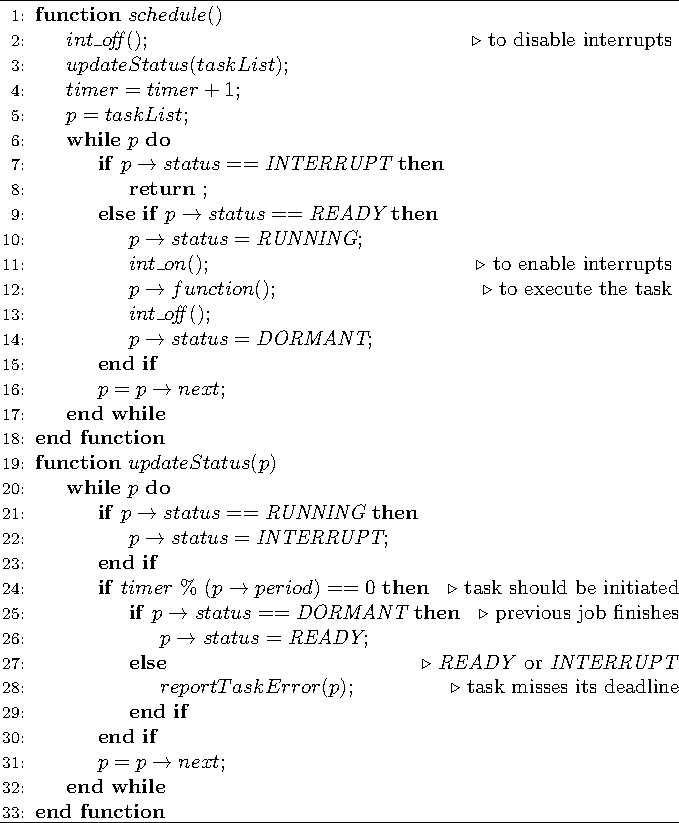
\includegraphics[width=0.9\textwidth]{FIG1_15-TIE-3480.pdf}
\caption{中断处理函数 $\mathit{schedule()}$ 的类 C 伪码}
\label{f:schedule}
\end{figure}

在图~\ref{f:schedule} 展示的伪码中,中断处理函数 $\mathit{schedule()}$ 首先通过调用函数 $\mathit{updateStatus()}$ 更新了 $\mathit{taskList}$ 中所有任务的状态。这个更新的动作,实际上对当前中断周期需要被调度的任务进行了初始化。然后 $\mathit{schedule()}$ 对链表 $\mathit{taskList}$ 进行遍历,对就绪的任务(状态为 \textit{READY})轮流予以执行,或者当遇到一个被中断的任务(状态为 \textit{INTERRUPT}\footnote{需要注意,状态 \textit{INTERRUPT} 表示该任务当前被中断,或者它曾经被中断而它目前仍未运行完毕。})时,进行返回操作(return)。由于 $\mathit{taskList}$ 中的任务是按优先级降序排列的,这样的遍历方式意味着调度从优先级高的任务开始。至于函数 $\mathit{updateStatus()}$,它对每一个任务的更新操作分为两步:首先,如果该任务正在运行(状态为 \textit{RUNNING}),则成为被中断状态;其次,当该任务处于应当进行初始化的时刻,如果该任务的上一个实例已经运行结束(状态为 \textit{DORMANT}),则变成就绪状态,否则意味着它错过了时限,将产生一个错误。需要注意,函数 $\mathit{schedule()}$ 仅仅在中断请求被处理时才会被调用。如果系统处于不可中断状态,即中断屏蔽标志位为 1,该函数则不会被调用。得益于中断屏蔽标志位,当函数 $\mathit{schedule()}$ 正在更新任务状态或寻找下一个该被运行的任务时,它不能被中断。然而,当它正在运行某个周期性任务时(第 12 行),它可以被中断。这就造成了函数 $\mathit{schedule()}$ 可能被嵌套调用。

为简便起见,本文用“调度过程”(scheduling)指代如下阶段:从中断请求被响应的时刻起,到第一个应当被运行的周期性任务开始运行(即图~\ref{f:schedule} 中第 8 行或第 12 行)的时刻止。因此,“调度开销”包括三部分:
\begin{enumerate}
\item 当中断请求被响应时,从正在运行的任务函数切换到 $\mathit{schedule()}$ 函数所耗费的上下文切换时间;
\item $\mathit{schedule()}$ 用于搜索\emph{第一个} 应当被运行的任务,以及准备运行该任务所花费的时间,对应图~\ref{f:schedule} 中第 2--11 行;
\item 从函数 $\mathit{schedule()}$ 切换到应当被运行的任务函数所耗费的上下文切换时间。
\end{enumerate}
“任务切换”(switching)指代以下阶段:从一个周期性任务实例完成其运行的时刻起,到下一个应当被运行的周期性任务开始运行的时刻止。同样,“任务切换开销”也包含三部分:
\begin{enumerate}
\item 当某个周期性任务实例运行完毕时,从该任务函数切换至 $\mathit{schedule()}$ 所耗费的上下文切换时间;
\item $\mathit{schedule()}$ 用于搜索\emph{下一个} 应当被运行的任务,以及准备运行该任务所花费的时间;
\item 从函数 $\mathit{schedule()}$ 切换到应当被运行的任务函数所耗费的上下文切换时间。
\end{enumerate}
 

\subsection{系统建模}
\label{s:formalism}


对硬件平台的部分技术细节(比如中断屏蔽技术)予以考虑,我们假设系统模型满足以下条件:

\begin{enumerate}
\item [(A1')] 任务 $\tau_i$ 的实例初始化时刻,等于在时刻 $kT_i$ 发出的时钟中断请求被响应的时刻,其中整数 $k\ge 0$;
\item [(A2)] 任意任务 $\tau_i$ 的运行时间 $C_i$ 是常数,它不随时间而改变;
\item [(A3)] 所有任务之间互相独立,使得它们在初始化的那一刻就可以被运行,并且随时可被其它任务抢占;
\item [(A4')] 系统的调度开销以及任务切换开销需要在模型中予以考虑,其它系统开销均被忽略。
\end{enumerate}


这些假设条件使我们的模型有别于标准 RMS 模型。比如说,根据假设条件~(A1'),如果中断请求出现在任务切换的过程中,那么它的响应将被推迟,使得 $\tau_i$ 的任务实例不能在时刻 $kT_i$ 进行初始化。它们将被推迟,直到任务切换过程结束时中断屏蔽位被清零。这与假设条件~(A1) 是不一样的。另一方面,条件~(A3) 假定任务实例在初始化时刻就进入就绪状态,随时可以被运行。然而,任何任务实例都不可能在初始化时刻就开始运行,因为调度过程也需要耗时。这些差别导致系统建模过程比标准 RMS 模型复杂,特别是对于硬件平台中断机制及系统开销的刻画。

\begin{figure}[ht]
\centering
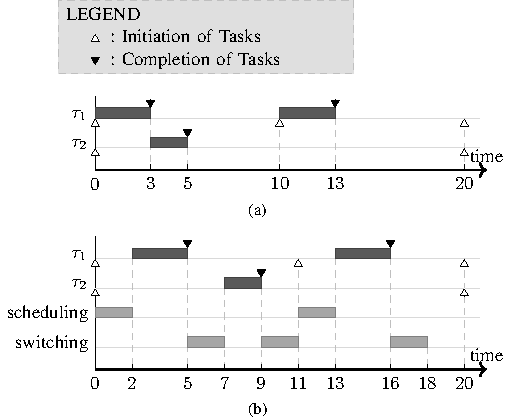
\includegraphics[width=0.7\textwidth]{FIG2_15-TIE-3480.pdf}
\caption{RMS 算法和 RMS 系统实现调度对比}
\label{f:example}
\end{figure}

根据这些假设条件,图~\ref{f:example}(b) 展示了图~\ref{f:example}(a) 的任务集在 RMS 系统实现中被调度的情况,其中假定调度开销和任务切换开销都为 2 个时间单位,时钟中断周期为 10。与图~\ref{f:example}(a) 不同,在图~\ref{f:example}(b) 中,在时刻 0,首先开始被运行的是调度过程。在经过了 2 个时间单位后,调度过程结束,优先级最高的 $\tau_1$ 才开始被运行。在时刻 5,当 $\tau_1$ 运行结束后,系统需要进行长达 2 个时间单位的任务切换,然后在时刻 7,任务 $\tau_2$ 才开始被运行。特别需要注意的是,在时刻 10,虽然有时钟中断请求发生,但因为正处于任务切换过程中,中断请求被屏蔽,中断响应被推迟。直到时刻 11 任务切换结束时,中断请求才被响应。$\tau_1$ 的初始化时刻是 11,而不是 10。这个行为展示了条件~(A1') 与 (A1) 的不同。

在本小节,我们将首先介绍如何利用带类型的项表达式来对系统状态建模,然后展示如何利用重写规则对系统的关键行为进行建模。特别需要指出,系统中的\emph{瞬时行为}(instantaneous  behaviors)将在第~\ref{ss:ir}、\ref{ss:init} 和~\ref{ss:inthandling} 小节进行解释;在第~\ref{ss:timedbehavior} 小节,将对系统的\emph{时间行为}(timed behaviors)进行解释。根据第~\ref{ss:realtime-modeling} 小节所述,系统中涉及时间的行为将利用 $\cR$ 规则进行描述,根据算法~\ref{alg:convert},即利用 Maude 的 $R$ 规则进行建模。

\subsubsection{基本类型}

在建立的系统模型中,任务将由它们在 $\mathit{taskList}$ 中的下标进行标识。所有下标具有自然数类型 \verb|Nat|。我们定义类型 \verb|MaybeNat| 对类型 \verb|Nat| 进行封装,用于指代任务集中的某个周期性任务。类型 \verb|MaybeNat| 具有两个\emph{构造子}(constructor):构造子 \verb|some| 带有类型为 \verb|Nat| 的参数 $n$,表示 $\mathit{taskList}$ 中第 $n$ 个任务;构造子 \verb|none| 指代“没有任务”。
\begin{verbatim}
  op none : -> MaybeNat [ctor] .
  op some_ : Nat -> MaybeNat [ctor] .
\end{verbatim}
其中关键字 \verb|ctor| 表示所对应的函数符号是构造子。

类型 \verb|Stack| 被定义用于对系统的栈结构进行建模。栈中存储的是被中断的任务(编号)。基于类型 \verb|Stack|,我们定义了栈操作 \verb|push|、 \verb|pop| 和 \verb|peek|。

类型 \verb|Counter| 被定义作为计数器,记录某个任务的\emph{已运行时间} 和运行时间。

在实际的代码中,$\mathit{schedule()}$ 函数的全局变量 $\mathit{timer}$ 在达到上界时将会被置 0。这一合理的技术细节没有在图~\ref{f:schedule} 进行展示,但包含在我们的模型中。$\mathit{timer}$ 的上界等于所有任务周期的最小公倍数。类型 \verb|Timer| 被定义用于对 $\mathit{timer}$ 进行建模。

\subsubsection{系统状态的建模}

整个对象系统可看作由以下几部分组成:被调度的任务集;RMS 调度模块;硬件平台,包括寄存器和栈;以及时钟中断源。其中 RMS 调度模块(即函数 $\mathit{schedule()}$)的状态可以只用单一变量 $\mathit{timer}$ 来表示。下面将给出其它部分的状态模型。

\paragraph{任务:} 由于我们的模型只关心调度问题,任务将被抽象成一个类型为 \verb|Counter| 的计数器。因为需要考虑调度过程和任务切换,这两个过程在模型中被当作两个\emph{系统任务}。每一个任务都被建模成基类 \verb|Task| 的某个子类的实例对象:
\begin{verbatim}
  class Task | cnt : Counter .
  op error : -> Object [ctor] .
\end{verbatim}
其中 \verb|error| 是用于表示某任务超时(即错过了时限)的实例对象。

被调度的周期性任务是类 \verb|PTask| 的实例。类 \verb|PTask| 是 \verb|Task| 的子类,具有额外的属性 \verb|priority|(表示任务优先级)、\verb|period|(表示任务周期)和 \verb|status|(表示任务状态):
\begin{verbatim}
  class PTask | priority : Nat, period : Nat, 
                status : Status .
  subclass PTask < Task .
\end{verbatim}
其中类型 \verb|Status| 具有四个常量构造子 \verb|RUNNING|、 \verb|INTERRUPT|、 \verb|READY| 和 \verb|DORMANT|,与图~\ref{f:schedule} 相对应。

周期性任务的链表(即系统实现中的变量 $\mathit{taskList}$)用类型 \verb|TaskList| 进行建模。\verb|TaskList| 是由 \verb|PTask| 的实例对象以及 \verb|error| 对象组成的列表结构。周期性任务由该列表中的元素下标进行标识。

另一方面,系统任务是类 \verb|SysTask| 的实例。类 \verb|SysTask| 也是 \verb|Task| 的子类,但没有额外的属性。与周期性任务不同的是,系统任务的集合具有类型 \verb|SysTasks|,而 \verb|SysTasks| 是多重集而非列表。系统任务由自身的对象标识 \verb|Oid| 进行标识。

\paragraph{硬件:} 我们的系统模型考虑了与中断处理有关的硬件部分——寄存器和栈。

寄存器被建模成类 \verb|Regs| 的实例。该类的属性 \verb|pc| 描述程序计数器 PC(Program Counter),属性 \verb|mask| 表示中断屏蔽标志位,属性 \verb|ir| 表示中断请求标志位: 
\begin{verbatim}
  class Regs | pc : TaskID, 
               mask : Bool, ir : Bool .
\end{verbatim}
其中,类型 \verb|TaskID| 包含子类型 \verb|MaybeNat| 和 \verb|Oid|,用于标识某个任务(包括周期性任务和系统任务)。类 \verb|Regs| 定义了对各属性的操作,如 \verb|getPc| 和 \verb|setMask| 等。 

于是硬件状态被建模成具有类型 \verb|Hardware| 的项表达式。\verb|Hardware| 由两部分构成:类 \verb|Regs| 的一个实例,和类型为 \verb|Stack| 的一个项表达式。

\paragraph{中断源:} 中断源被建模成类 \verb|IntSrc| 的一个实例。类 \verb|IntSrc| 具有两个属性:\verb|cycle| 表示时钟中断周期 $T$;\verb|val| 的数值随着时间推移从 $T$ 递减为 $0$。
\begin{verbatim}
  class IntSrc | val : Time, cycle : Time .
\end{verbatim}

\paragraph{系统状态:} 在我们的模型中,系统状态由以上部分组合构成,具有类型 \verb|System|\footnote{根据 Maude 的使用习惯,变量符号将由大写字母表示。为了易于阅读,变量声明语句在此省略。}:
\begin{verbatim}
  op _____ : TaskList Timer SysTasks 
             Hardware Object ~> System [ctor] .
  mb (L T STS HW < O : IntSrc |>) : System .
\end{verbatim}
其中,“\verb|~>|” 表示该函数符号是个\emph{部分函数}(partial function);关键字 \verb|mb| 声明一种\emph{成员关系}(membership),在这里表示,如果一个项表达式由 \verb|TaskList|(周期任务列表)、\verb|Timer|(变量 $\mathit{timer}$)、\verb|SysTasks|(系统任务集合)、\verb|Hardware|(硬件) 以及类 \verb|IntSrc| (中断源) 的实例构成,那么它具有类型 \verb|System|。

\subsubsection{中断请求}
\label{ss:ir}

当属性 \verb|val| 的值递减为 0 时,中断请求由中断源触发。中断请求每隔周期 $T$ 将会发出一次。请求的动作是瞬间完成的,因此将由以下瞬时条件重写规则进行建模。该规则作用于类型为 \verb|System| 的项表达式:
\begin{verbatim}
  crl [interrupt-request] :
    (L T STS HW ISRC) 
    => (L T STS (HW).intReq reset(ISRC))
    if (ISRC).timeout .
\end{verbatim}
其中,函数 \verb|_.timeout| 检查属性 \verb|val| 的值是否为 0;函数 \verb|_.intReq| 将属性 \verb|ir| 置 1,表示当前存在中断请求需要被响应。

然后该中断请求将等待被响应处理,其过程的建模将在第~\ref{ss:inthandling} 小节进行解释。

\subsubsection{任务初始化}
\label{ss:init}
周期性任务将按顺序被图~\ref{f:schedule} 中的函数 $\mathit{updateStatus()}$ 进行初始化。这一过程在我们的模型中被看作一个瞬时行为。它将由以下函数 \verb|updateStatus_with_| 进行建模:
\begin{verbatim}
  op updateStatus_with_ : TaskList Timer 
                            -> TaskList . 
\end{verbatim}
该函数对 $\mathit{taskList}$ 中的任务逐一应用函数 \verb|update_with_|,使任务状态得到更新(对应图~\ref{f:schedule} 的第 21--30 行):
\begin{verbatim}
  op update_with_ : Object Timer ~> Object .
  ceq update < O : PTask | period : T, 
                           status : ST > 
        with TIMER
      = if ST == DORMANT 
        then < O : PTask | status : READY >
        else error fi
      if TIMER rem T == 0 .
  eq update < O : PTask | status : ST > 
       with TIMER
     = if ST == RUNNING 
       then < O : PTask | status : INTERRUPT >
       else < O : PTask |> fi [otherwise] .
\end{verbatim}
其中变量符号 \verb|TIMER| 表示全局变量 $\mathit{timer}$ 的值。给定一个周期性任务,如果 \verb|TIMER|(即 $\mathit{timer}$)可被任务周期 \verb|T| 整除,那么该任务需要被初始化。在任务需要被初始化的情况下:如果它处于空闲状态(\verb|DORMANT|),则将进入就绪状态(\verb|READY|);否则意味着该任务的上一个任务实例没有运行完毕,因此该任务超时,产生 \verb|error| 对象。在任务不需要被初始化的情况下,只有当其处于运行状态(\verb|RUNNING|)时,任务状态才需要被改变。

通过对比可以看出,模型中的函数 \verb|updateStatus_with_| 具有与图~\ref{f:schedule} 中函数 $\mathit{updateStatus()}$ 相同的行为。

\subsubsection{中断处理与任务调度}
\label{ss:inthandling}

当中断请求发生时,它可能不会马上被系统检测到。中断请求的检测要求中断屏蔽标志位 \verb|mask| 为 0。一旦系统检测到存在中断请求,中断的处理分为两步:首先是硬件对中断信号的处理,比如清空中断请求标志位 \verb|ir|、将当前函数的上下文压栈等;然后是调用中断处理函数 $\mathit{schedule()}$。这个过程用以下瞬时重写规则进行建模:
\begin{verbatim}
  crl [interrupt-handle] :
    SYSTEM 
    => ((SYSTEM).interrupt).startScheduling
    if (SYSTEM).existInt .
\end{verbatim}
其中,函数 \verb|_.existInt| 检查 \verb|mask| 是否为 0 \emph{且} \verb|ir| 为 1。函数 \verb|_.interrupt| 对硬件的中断处理机制进行建模,它进行了四步操作:
\begin{enumerate}[(i)]
\item 清空标志位 \verb|ir|,表示中断请求已被响应;
\item 将当前程序计数器 \verb|pc| 压进栈中,保存被中断的上下文;
\item 将 \verb|pc| 的值设成具有类型 \verb|Oid| 的项表达式 \verb|scheduling|,表示系统正处于调度阶段;
\item 将中断屏蔽标志位 \verb|mask|置 1,屏蔽即将到来的中断请求。
\end{enumerate}

与周期性任务不同,虽然调度过程也作为系统任务被建模成一个计数器 \verb|Counter|,但因其功能过于重要,以至于不能将其功能完全抽象化。我们将调度过程的行为划分为三部分。第一部分包含了调度过程的时间行为。这一部分通过将调度过程看作一个系统任务(类型为 \verb|SysTask|)来描述其时间行为。时间行为的建模将在第~\ref{ss:timedbehavior} 小节中详述。其它两部分共同定义了调度过程的功能。第二部分对应于图~\ref{f:schedule} 的第 3--4 行。它更新了 $\mathit{taskList}$ 的状态并且给 $\mathit{timer}$ 加 1。这一部分行为被建模成函数 \verb|_.startScheduling|。它将在调度过程的开始时刻作为瞬时动作发生,如以下规则 \verb|interrupt-handle| 所示:
\begin{verbatim}
  op _.startScheduling : System -> System .
  eq (L T STS HW ISRC).startScheduling 
     = ((updateStatus L with T) 
        inc(T) STS HW ISRC) .
\end{verbatim}
第三部分对应于图~\ref{f:schedule} 的第 6--11 行,它负责搜索第一个应该被运行的周期性任务,并准备予以执行。这部分行为被建模成函数 \verb|_.finishScheduling|,并在调度过程的结束时刻作为瞬时动作发生:
\begin{verbatim}
  op _.finishScheduling : System -> System .
  eq (L T STS HW ISRC).finishScheduling
     = (L T (finish scheduling in STS) 
        HW ISRC).run1stTask .
\end{verbatim}
其中,函数 \verb|finish_in_| 重置系统任务 \verb|scheduling| 的计数器;函数 \verb|_.run1stTask| 对第 6--11 行建模,从状态为 \verb|INTERRUPT| 或 \verb|READY| 的任务中找到优先级最高的任务,根据其状态分别进行\emph{中断返回}(interrupt return)或执行动作。

当系统任务 \verb|scheduling| 的已运行时间达到它的运行时间时,调度过程结束。我们用以下规则建模这一瞬时行为:
\begin{verbatim}
  crl [scheduling-finish] :
    SYSTEM => (SYSTEM).finishScheduling
    if SYSTEM := (L T STS HW ISRC) 
       /\ (SYSTEM).running == scheduling 
       /\ scheduling isComplete?in STS .
\end{verbatim}
其中,函数 \verb|_.running| 返回当前系统的 \verb|pc| 值,即正在运行的任务标识;而函数 \verb|_isComplete?in_| 检查该任务的已运行时间是否已达到其运行时间。

与调度过程类似,任务切换过程 \verb|switching| 也被划分为时间行为与其功能行为。当正在运行的周期性任务运行结束时,系统任务 \verb|switching| 开始运行,直到自身的已运行时间达到自身的运行时间。两条类似的瞬时规则 \verb|switching-start| 和 \verb|switching-finish| 被用于对任务切换过程的功能行为进行建模。


\subsubsection{系统的时间行为}
\label{ss:timedbehavior}

系统的时间行为由两部分构成:所有任务的运行和时钟中断源的运行。两者可以同时被以下\emph{标准} 的\emph{单元计时规则}~\cite{DBLP:journals/entcs/OlveczkyM07a}(tick rule)所建模\footnote{关键字 \texttt{nonexec} 允许 Real-Time Maude 根据某种策略来应用重写规则。}:
\begin{verbatim}
  crl [tick]:
    {SYSTEM} => {delta(SYSTEM, R)} in time R 
    if R le mte(SYSTEM) [nonexec] .
\end{verbatim}
其中,函数 \verb|delta| 定义了时间推移对系统状态产生的效果;函数 \verb|mte| 表示的是,从当前时刻直至任意瞬时动作\emph{必须} 发生的时刻,系统允许的\emph{最大时间推移量} (Maximum amount of Time allowed to Elapse)。实际上,对系统时间行为建模的关键就在于定义函数 \verb|delta| 和 \verb|mte|。需要注意的是,变量 \verb|R| 相对于我们所指定的时间域\footnote{Real-Time Maude 包含了预定义的模块用于指定时间域是自然数集或是实数集,而这两者分别定义了\emph{离散} 的时间域和\emph{连续} 的时间域。}(time domain)来说是\emph{连续的}(continuous)。

时间推移对我们的目标系统的影响是,它使 \verb|pc| 指定的任务和时钟中断源的状态随着时间推移在向前推进。具体的表现是,当时间向前推移,正在运行的任务的计数器 \verb|cnt| 在递增,而中断源的 \verb|val| 值在递减:
\begin{verbatim}
  ceq delta((L T STS HW ISRC), R)
      = (deltaTask(ID, L, R) 
         T STS HW (deltaIS(ISRC, R)))
      if ID := (HW).getPc /\ ID :: MaybeNat .
\end{verbatim}
其中,规则的最后一个条件表示 \verb|ID| 的类型为 \verb|MaybeNat|,即表示当前正在运行的任务为周期性任务。类似地,如果 \verb|ID| 的类型为 \verb|Oid|,即当前运行的任务为系统任务,那么函数 \verb|deltaTask| 将作用于 \verb|STS| 而非 \verb|L|。

\verb|mte| 取决于下一个强制发生的瞬时动作的时刻。因此,它由三个因素决定:还有多长时间能完成当前正在运行的任务;还有多长时间产生下一个中断请求;当前是否有中断请求被系统检测到。
\begin{verbatim}
  ceq mte(L T STS HW ISRC)
      = minimum(mteTask(ID, L),
                mteIS(ISRC), mteIr(HW))
      if ID := (HW).getPc /\ ID :: MaybeNat .
\end{verbatim}
其中,如果当前存在中断请求被系统检测到,函数 \verb|mteIr| 将返回 0;否则返回 \verb|INF|,表示\emph{无穷}(infinity)。当 \verb|ID| 为类型 \verb|Oid| 时,情况类似。


\subsection{形式化验证}
\label{s:verification}
在本小节,我们针对不同的真实场景,对 RMS 系统的重写模型进行分析。需要注意,得益于 $\mathit{timer}$ 的上界,从任意(合理的)初始状态出发,该模型的可达状态数是有限的。这使得我们可以应用非时控的模型检测器对模型进行形式化验证。

\subsubsection{验证属性}
本案例我们考虑两个验证属性:可调度性和正确性。通过可调度性,我们验证一个给定的周期性任务集合在该 RMS 系统的调度下是否满足可调度性。通过正确性,我们验证该 RMS 系统对周期性任务的调度方式是否按照 RMS 算法的规范进行。

为了验证可调度性,我们定义原子命题 \verb|taskTimeout|。\verb|taskTimeout| 成立的条件是在当前状态中,$\mathit{taskList}$ 包含 \verb|error| 对象,即某个任务发生超时:
\begin{verbatim}
  op taskTimeout : -> Prop [ctor] .
  eq {L T STS HW ISRC} |= taskTimeout 
     = containError(L) .
\end{verbatim}
其中,函数 \verb|containError| 返回 \verb|true| 当且仅当 \verb|L| 中存在 \verb|error|。 可调度性可以被形式化地描述成时序逻辑公式 \verb|[](~taskTimeout)|,它表示命题 \verb|taskTimeout| 总是不成立。由于该性质与时钟无关(clock-unrelated),给定初始状态 \verb|init|,以下非时控模型检测命令可以用于验证可调度性是否在任意时刻总是成立。如果成立,该命令返回 \verb|true|;否则,该命令返回一条反例路径:
\begin{verbatim}
  (mc init |=u [](~taskTimeout) .)
\end{verbatim}

本案例另外一个重要目的是验证该系统实现的正确性。我们定义原子命题 \verb|correct|,它成立的条件是,当前运行的周期性任务是所有请求运行的周期性任务中优先级最高的:
\begin{verbatim}
  op correct : -> Prop [ctor] .
  ceq {L T STS HW ISRC} |= correct
      = if ID :: MaybeNat then shouldRun(ID, L)
        else true fi
      if ID := (HW).getPc .
\end{verbatim}
其中,函数 \verb|shouldRun(ID, L)| 返回 \verb|true| 的条件是,标识为 \verb|ID| 的任务在当前所有非空闲状态的任务中具有最高优先级。需要注意的是,在系统的运行过程中,如果存在任务超时,我们的验证需求不关心任务超时后的行为(比如错误恢复等)。因此,实现正确性可以被以下时序逻辑公式描述:\verb|([]correct)\/(correct U taskTimeout)|,表示 \verb|correct| 总是成立,或者保持成立直到命题 \verb|taskTimeout| 成立。给定初始状态 \verb|init|,正确性能被以下非时控模型检测命令所验证:
\begin{verbatim} 
  (mc init |=u ([]correct) 
               \/ (correct U taskTimeout) .)
\end{verbatim}

\subsubsection{验证场景}
\label{ss:results} 
我们在验证过程中使用以下参数配置,数据来源于我们的工业合作伙伴提供的真实数据:
\begin{itemize}
\item 时钟中断周期 $T$ 为 $5ms$;
\item 调度开销为 $38{\mu}s$,任务切换开销为 $20{\mu}s$;
\item 初始状态的栈为空,程序计数器 \verb|pc| 为空,中断屏蔽标志位 \verb|mask| 为 0,中断请求标志位 \verb|ir| 为 0。
\end{itemize}

我们在 10 种不同的场景下对我们的模型进行了验证。其中既包括我们的合作伙伴提供的真实场景,也包括我们自己设计的实验场景。其中四个场景描述如下:
\begin{itemize}
\item 场景 (i) 包含2个任务 $\tau_1$ 和 $\tau_2$: $T_1=5ms$, $C_1=3ms$, $T_2=25ms$, $C_2=7ms$;
\item 场景 (ii) 包含 2 个任务 $\tau_1$ 和 $\tau_2$: $T_1=5ms$, $C_1=2ms$, $T_2=25ms$, $C_2=2.3ms$;
\item 场景 (iii) 包含 3 个任务 $\tau_1$、$\tau_2$ 和 $\tau_3$:$T_1=5ms$, $C_1=2.7ms$, $T_2=10ms$, $C_2=2ms$, $T_3=25ms$, $C_3=3ms$;
\item 场景 (iv) 包含 3 个任务 $\tau_1$、$\tau_2$ 和 $\tau_3$:$T_1=5ms$, $C_1=2.5ms$, $T_2=10ms$, $C_2=1.5ms$, $T_3=15ms$, $C_3=4.5ms$。
\end{itemize}
值得注意的是,得益于 Real-Time Maude 丰富的表达能力,对不同的任务集合,只需定义不同的初始状态(\verb|System| 类型)即可,不需对模型本身进行修改和调整。

在验证的过程中,我们的模型选择了连续的时间域以及\emph{极大时间采样策略}(maximal time sampling strategy)。模型检测的结果显示,正确性在所有场景中成立。而对于可调度性,它在场景 (i--iii) 成立,但在场景 (iv) 中不成立。我们将模型检测命令返回的反例路径绘成图~\ref{f:counterexample}。从图中可以看到,在第 $15ms$ 时,任务 $\tau_3$ 的第一个实例还没有完成运行,而此时它的第二个任务实例进行初始化,于是发生了超时,可调度性不成立。

\hide{
以上结果展示了我们的方法在真实工业系统中的可用性。然而,为了检验此方法的效率,我们进一步尝试将我们的方法应用于规模更大的实验场景中。
实验场景完全随机产生。我们在上述参数配置下验证随机实验场景的可调度性。进行验证的机器配置为:英特尔酷睿 2 Quad Q9550,2.83GHz,4 核,8GB 内存,64 位 Ubuntu
15.04 操作系统。 在50个随机生成的包含5个周期性任务的实验场景中,我们发现各场景的验证时间差别极大,从 $300ms$ 到超时(超时时间设为90分钟)不等。
这是由于模型检测的效率取决于状态空间的规模。而在我们的模型中,状态空间的规模与
 $mn$ 正相关,其中 $m$ 是变量 $\mathit{timer}$ 的上界,$n$ 是周期任务的数量。
对这些随机实验场景的验证结果表明,我们的方法在90分钟内能处理的场景规模大约为 $mn$ 等于  $10^6$。
}

\subsubsection{结果评估}
本小节将说明我们的验证结果是可靠且完备的。

给定一个验证方法,如果这个方法产生的任何反例都是原问题的真正反例,则称这个验证方法是\emph{可靠的};如果应用该方法没有找到反例,能说明原问题也不存在反例,则称这个验证方法是\emph{完备的}。要判断我们的方法是否可靠很简单,只需要检查产生的反例是否真反例。比如,图~\ref{f:counterexample} 的反例是真反例,这表明关于场景~(iv) 可调度性的验证结果是可靠的。然而需要证明完备性,却不太简单。我们的模型选择了连续时间域,使其行为更加贴近真实系统。然而这一选择也导致了系统的状态空间成为无穷大,不可能穷尽所有状态。

\begin{landscape}
\begin{figure}[t]
\centering 
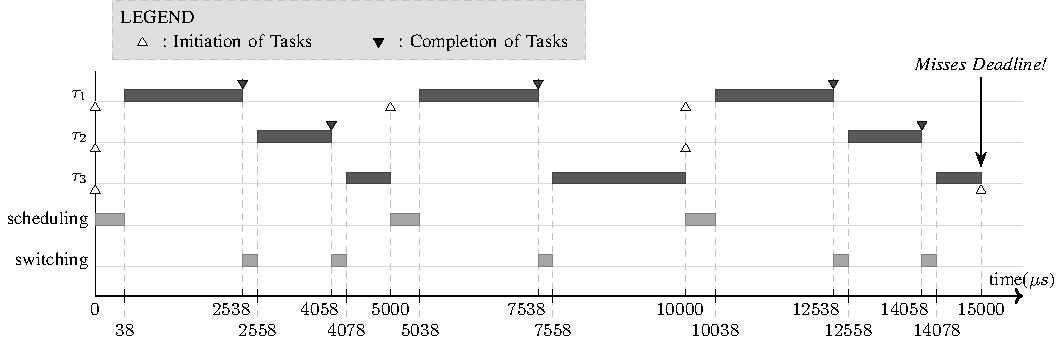
\includegraphics[width=1.5\textwidth]{FIG3_15-TIE-3480.pdf}
\caption{场景 (iv) 可调度性的反例}
\label{f:counterexample}
\end{figure}
\end{landscape}

一般来说,我们没有办法证明非时控的模型检测方法对任意系统、任意时间采样策略以及任意验证属性都具有完备性。然而, \"Olveczky 和 Meseguer 证明了非时控的时序逻辑模型检测方法,在应用极大时间采样策略对“某类”实时系统进行“某类”LTL 公式的验证时,是完备的~\cite{DBLP:journals/entcs/OlveczkyM07a}。“这类”实时系统称作\emph{时间鲁棒的}(time-robust),而“这类”LTL 公式由\emph{单元计时不变的}(tick-invariant)命题构成\footnote{在此我们避免引入时间鲁棒性和单元计时不变性的准确定义,因为这需要更深入的重写逻辑背景知识。}。

\begin{theorem}[\inlinecite{DBLP:journals/entcs/OlveczkyM07a}]
\label{t:completeness}
给定一个时间鲁棒的实时重写逻辑模型 $\mathcal{R}^{\cL}$,一个单元计时不变的原子命题集合 $AP$,一个由 $AP$ 中命题构成的 LTL 公式 $\Phi$ (不包含 $\bigcirc$ 操作符)。那么非时控的时序逻辑模型检测方法在应用极大时间采样策略对 $\Phi$ 进行验证时,它是\emph{完备的}。
\end{theorem}

因此,我们可以证明以下定理,表明第~\ref{ss:results} 小节的验证结果是完备的。
\begin{theorem}
\label{t:main}
采用非时控模型检测方法去验证本案例的系统模型的可调度性和正确性,所得结果是完备的。
\end{theorem}
\begin{proof}
首先证明我们的模型是时间鲁棒的;其次证明我们定义的原子命题 \verb|taskTimeout| 和 \verb|correct| 是单元计时不变的;最后应用定理~\ref{t:completeness} 得到结论。更详细的证明,请参见附录~\ref{app:proof}。
\end{proof}




\subsection{相关工作}
\label{s:relate}
在本小节,我们从三个方面来对本案例应用及其相关工作进行对比。

先从可调度性判定的角度来说,Liu 和 Layland 给出了一个最常用的充分条件:一个周期性任务集合如果满足 $\Sigma^n_{i=1} C_i/T_i \le n(2^{1/n}-1)$,那么它根据 RMS 算法是可调度的~\cite{DBLP:journals/jacm/LiuL73}。然后,Bini 等人提出了一个更有效的充分条件~\cite{DBLP:journals/tc/BiniBB03},它具有跟前者同样的算法复杂度。在另一方面,判定可调度性的充分必要条件由 Sprunt 等人~\cite{DBLP:journals/rts/SpruntSL89} 及 Audsley 等人~\cite{audsley1993deadline} 分别提出,要求对任务集合进行更复杂的分析。然而,所有这些分析都建立在理想的模型上,并不考虑系统开销,真实性不如本文建立的模型。Katcher 等人基于几种主流的 RMS 实现方法,在可调度性分析中考虑了系统开销~\cite{DBLP:journals/tse/KatcherAS93}。然而,本案例的目标系统不在他们的考虑范围之内。此外,相比于那些理论的分析,本文采用的基于形式化建模与验证的分析方法主要有三个优点。一是如果我们的可调度性检查给出系统“不可调度”的结果,它同时能够返回一条反例路径。这条反例路径可以指导开发人员调整系统设计,比如调整任务优先级、甚至改变调度算法。第二个优点是,如果想要在系统中应用一个全新的调度策略,本小节的分析方法只需要对模型进行修改就能对新策略进行分析,而理论分析方法则需要重新进行分析和推理。最后一个优点是,在分析中考虑系统开销和硬件细节会给模型引入不确定性。比如在我们的模型中,如果正在运行的任务\emph{恰好} 在中断请求发生时完成运行,则将可能发生两种不同的行为:(i)~系统进行任务切换,在任务切换过程中中断请求被屏蔽,因此调度过程和任务的初始化将被推迟;(ii)~系统立即响应该中断请求,则任务切换将被推迟。相比于本案例的自动验证方法,对这些不确定行为进行理论分析要复杂得多。

Tian 和 Duan~\cite{TianD2011} 以及 Cui 等人~\cite{DBLP:conf/iceccs/CuiDT14} 以类似的方法,利用模型检测技术对 RMS 算法进行了分析。与本案例不同的是,这两项工作使用了不同的建模语言和工具。Tian 和 Duan 使用 SPIN~\cite{DBLP:journals/tse/Holzmann97} 的一类扩展对 RMS 算法进行建模和验证~\cite{TianD2011};而 Cui 等人则使用了逻辑编程语言 TMSVL~\cite{DBLP:conf/icfem/HanDW12} 及其模型检测工具~\cite{DBLP:conf/iceccs/CuiDT14}。这两项工作与本工作存在两个主要区别。首先,最重要的区别在于,这两项工作的分析对象都是 RMS 算法的标准理想模型~\cite{DBLP:journals/jacm/LiuL73},而不是包含了更多复杂细节的系统实现,这也是本案例应用的主要出发点。实际上,如果我们假设调度过程和任务切换的时间等于 0,那么标准的 RMS 模型将成为我们的 RMS 系统模型的特例。因此,本案例建立的模型更具一般性。另外一个区别在于,如果需要在周期任务集合中添加一个新任务,Tian 和 Duan 的模型~\cite{TianD2011} 以及 Cui 等人的模型~\cite{DBLP:conf/iceccs/CuiDT14} 都需要进行修改,为新任务及其行为增加一个子模块。特别需要指出的是,Tian 和 Duan 模型中的调度部分同样需要调整以增加新任务~\cite{TianD2011}。然而,在我们的模型中,增加新任务只需要修改初始状态即可,模型不需作任何修改。这一点已经在第~\ref{ss:results} 小节中指出。另一方面,Tian 和 Duan 在模型中使用离散时间域~\cite{TianD2011},而我们的模型则使用了参数化的时间域,允许实例化成离散时间域或连续时间域,非常灵活。Cui 等人也使用了连续的时间域,同时采用建模策略以减少状态空间规模~\cite{DBLP:conf/iceccs/CuiDT14},与本工作的极大时间采样策略类似。但我们证明了此方法的完备性(定理~\ref{t:main}),而 Cui 等人没有给出类似结论。

最后, Maude 和 Real-Time Maude 目前已成功地被应用到诸多领域~\cite{DBLP:journals/jlp/Meseguer12},特别是通信协议、安全协议。但还没有被应用于分析调度问题。据我们所知,这是首次利用 Real-Time Maude 分析 RMS 算法及其实现。


\subsection{案例小结}
\label{s:conclusion} 
在本案例应用中,我们利用 Real-Time Maude 对一个真实的 RMS 系统进行了建模。在建立的系统模型中,我们考虑了调度及任务切换所产生的系统开销,也考虑了硬件平台的部分细节。我们的模型包含了足够多的细节对真实的目标系统行为进行描述。通过对建立的模型应用模型检测技术,我们在不同的关键场景下验证了系统的可调度性和正确性。最后我们证明了验证结果是可靠且完备的。在该案例中经过我们建模验证的 RMS 系统目前在某工业级航天控制器中在线运行。


\section{本章小结}

本章基于已有的重写逻辑建模验证工作,针对嵌入式系统的特性,如结构层次化、高度并发、并发行为与顺序行为并存、系统结构动态变化、实时性等,提出了基于规范化条件重写模型的建模方法。通过模型层面的语义映射,我们将该建模方法在工具集 Maude 中予以实现。利用该方法,我们对两个真实的嵌入式系统——机车优化控制系统和速率单调调度系统进行了建模分析。对于前者,我们应用了测试与验证相结合的方法,成功发现系统中的潜在缺陷,提高了系统的可靠性;该系统目前运行稳定,并在沈阳铁路局通过了实车运用考核。而对于后者,我们应用模型检测技术对系统的可调度性和正确性进行了形式化验证,并证明了其结果具有可靠性和完备性;经验证的 RMS 系统目前在某工业级航天控制器中在线运行。这两个应用案例表明了本章提出的建模方法在实际系统应用中具有可行性。

\chapter{C 语言程序终止性的自动验证}
\label{cha:c-termination}

上一章从建模方法论的角度,试图提高规范化条件重写模型作为一种建模模型的易用性。本章将从另外一个角度切入,进一步降低利用规范化条件重写模型进行建模验证的成本。在此前的讨论中,建模过程不针对任何特定的验证属性。这要求建立的模型应尽可能涵盖系统各方面的行为特征,并包含尽可能多的细节,使得针对模型任何属性的验证结果都可以代表系统的性质。因此,为了保证模型与系统的等价性以及抽象程度的合理性,建模过程只能通过人工进行。然而,如果只针对某种特定属性,如可达性、终止性等,则建模过程只需要针对系统行为的某个侧面进行。这将显著地降低建模的难度,使得建模过程的自动化成为可能。

本章在已有对 C 语言程序自动建模的工作基础上,开发实现了针对 C 语言程序终止性的自动验证工具 \CTerm。

\section{引言}

程序的终止性问题是验证领域的一个重要问题。它的重要性主要体现在两个方面。首先,终止性是完全正确性(Total correctness)的必要条件。一个程序(或算法)被称作完全正确,当且仅当它是终止的,且它的行为符合其规约(Specification)的规定。用 Hoare 逻辑~\cite{DBLP:journals/cacm/Hoare69} 表示,三元组 $\{P\}~\texttt{C}~\{Q\}$ 成立,当且仅当在满足谓词 $P$ 的前提下,(i) 程序 $\texttt{C}$ 终止;且 (ii) 执行完 $\texttt{C}$ 后谓词 $Q$ 成立。而一个程序(或算法)称作部分正确,则只要求在假设它终止的前提下,其行为符合规约的规定。也就是说,三元组 $\{P\}~\texttt{C}~\{Q\}$ 成立,当且仅当在满足谓词 $P$ 的前提下,如果程序 \verb|C| 终止,则执行完 $\texttt{C}$ 后谓词 $Q$ 成立。举以下简单例子:
\begin{verbatim}
    {x == 1} while (true) x = x; {y == 2}
\end{verbatim}
由于其 \verb|while| 循环不终止,该程序根据其规约,不是完全正确的,但它是部分正确的。

程序终止性的第二个重要性在于,对 CTL~\cite{DBLP:conf/lop/ClarkeE81}、CTL*~\cite{DBLP:journals/jacm/EmersonH86}、Fair-CTL~\cite{DBLP:journals/jcss/EmersonH85} 以及 LTL~\cite{DBLP:conf/banff/Vardi95} 性质的验证,可以转化为对安全性~\cite{DBLP:journals/tse/Lamport77}(safety)和对终止性的验证~\cite{DBLP:conf/tacas/BrockschmidtCIK16}。由于目前大多数程序验证工具都针对安全性进行验证,因此终止性验证工具的研究理论上可以提升这些程序验证工具的验证能力。

嵌入式系统的软件部分通常由 C 语言进行实现,因此开发 C 语言程序的终止性自动验证工具,对保障嵌入式系统的可靠性具有重要意义。

程序的终止与否,有时候并不容易判断,如以下例子(Collatz 问题):
\begin{verbatim}
    while (x > 1) {
      if (even(x))  x = x / 2;
      else  x = 3 * x + 1;
    }
\end{verbatim}
目前有许多技术可以自动验证一个程序的终止性,而其中一种主流技术正是基于整数重写模型~\cite{DBLP:conf/rta/FalkeKS11}。整数重写模型可以看作是规范化条件重写模型的一种特例。在第~\ref{cha:normalrewriting} 章已经提到,重写模型的终止性是该领域的最重要问题之一,目前已经有大量关于重写模型终止性的验证理论及工具。通过将程序(自动)建模成整数重写模型,程序终止性问题就可以被转化为重写模型的终止性问题,从而使用对应的技术进行解决。本文基于这种技术路线,开发了 C 语言程序终止性自动验证工具 \CTerm。

本章其余部分组织结构如下:第~\ref{s:termination-related} 小节介绍相关的 C 程序终止性自动验证工具;第~\ref{s:termination-models} 小节讨论如何自动建立 C 程序的整数重写模型,以便对程序终止性进行验证;\CTerm 工具将在第~\ref{s:ceagle-termination} 小节进行介绍;最后对本章内容进行简要小结。 

\section{相关工作}
\label{s:termination-related}

对指令式程序的终止性进行自动验证,目前主要有三种主流技术。 

排序函数~\cite{DBLP:conf/lics/PodelskiR04}(ranking function)是最经典的用于证明程序终止性的技术。排序函数 $rank$ 将每一个程序状态 $s$ 映射为抽象域(如正整数域)中的一个元素 $rank(s)$。如果对于程序的每一步执行 $s \ra s'$,排序函数满足 $rank(s) > rank(s')$,且抽象域上的二元关系 $>$ 是良基的(Well-founded),即不存在无穷递减序列,则该程序是终止的。于是验证程序终止性的问题可以被归约为排序函数的构造问题。如果满足条件的排序函数存在,则可判断该程序终止。基于排序函数构造的自动验证工具主要有 \textsc{OctaTerm}~\cite{DBLP:conf/popl/BerdineCCDO07}、\textsc{PolyTerm}~\cite{DBLP:conf/popl/BerdineCCDO07}、FuncTion~\cite{DBLP:conf/sas/Urban13,DBLP:conf/tacas/Urban15} 和 \textsc{c2fsm+Aspic+Rank}~\cite{DBLP:conf/sas/AliasDFG10}。其中 \textsc{OctaTerm} 和 \textsc{PolyTerm} 并不支持 C 程序的输入,而 FuncTion 和 \textsc{c2fsm+Aspic+Rank} 可以支持。

针对排序函数构造困难的问题,ARMC~\cite{DBLP:conf/padl/PodelskiR07}、CProver~\cite{DBLP:conf/cav/KroeningSTW10,DBLP:conf/tacas/TsitovichSWK11}、TERMINATOR~\cite{DBLP:conf/pldi/CookPR06} 及其后继工具 T2~\cite{DBLP:conf/tacas/BrockschmidtCIK16} 等 C 程序终止性验证工具采用了递增式的排序函数构造技术。这些工具将安全性检查过程集成到排序函数的构造过程中。其主要原理是,若当前已经有排序函数 $rank$ 对程序的某些执行序列满足递减关系,则利用安全性检查工具找到一条不能使 $rank$ 递减的执行序列 $\pi$;根据反例 $\pi$ 对 $rank$ 进行改善,得到新的排序函数 $rank'$。重复此过程直到构造的排序函数能使程序的所有执行序列满足递减关系。同样基于排序函数结合安全性检查技术的 C 程序终止性验证工具还有 \textsc{SeaHorn}~\cite{DBLP:conf/tacas/UrbanGK16} 和 2LS~\cite{DBLP:conf/kbse/ChenDKSW15}。在 \textsc{SeaHorn} 的实现中,安全性检查技术的使用方式与其它工具稍有不同,目的是为了在对当前排序函数进行改善时,能获得更多信息。而 2LS 则将过程间分析技术加入到排序函数的构造过程中。 
 
另一个主流技术是将程序的终止性验证问题归约为重写模型的终止性判定问题。通过利用重写模型(或其扩展形式)对程序中影响终止性的行为进行自动建模,若模型具有终止性,则可判定该程序也具有终止性。这种技术方案的好处是可以充分利用重写领域对终止性的判定技术,如递归路径序~\cite{DBLP:journals/jsc/Dershowitz87}(Recursive path order)、Knuth-Bendix 序~\cite{knuth1983simple}(Knuth-Bendix order)、依赖对~\cite{DBLP:journals/tcs/ArtsG00,DBLP:journals/jsc/GieslAO02}(Dependency pair)等。基于这种技术方案的 C 程序终止性验证工具主要有 AProVE~\cite{DBLP:conf/cade/GieslBEFFOPSSST14}、\verb|llvm2KITTeL|+\verb|KITTeL|~\cite{DBLP:conf/rta/FalkeKS11}(以下简称为 \verb|KITTeL|) 和 c2lctrs+Ctrl~\cite{DBLP:conf/lpar/Kop015,KN15}(以下简称为 Ctrl)。其中 \verb|KITTeL| 和 Ctrl 的模型直接从 C 程序的控制流图中进行抽取,因此无法对涉及指针的程序行为进行描述。而 AProVE 先通过符号执行技术构造程序的一种中间表示形式——符号执行图(Symbolic execution graph),然后再从中抽取重写模型。由于符号执行图包含了程序中涉及指针的行为,因此 AProVE 的技术方案能更好地处理包含内存操作的 C 程序。

近年来也出现了一些新兴的技术可用于验证 C 程序的终止性。例如工具 HipTNT+~\cite{DBLP:conf/pldi/LeQC15} 实现了一种基于函数摘要(Summary)的终止性验证技术,通过推理得到每个函数的终止性或非终止性的摘要,然后综合得到整个程序的终止性验证结果。Ultimate B\"uchi Automizer~\cite{DBLP:conf/cav/HeizmannHP14} 实现了一种基于程序构造的终止性验证技术。它首先对程序进行执行路径采样,得到若干套索形状(Lasso-shaped)的程序执行路径;然后根据这些路径构造出若干具有终止性的程序片段;重复该过程直到构造出来的程序片段集合可以涵盖目标程序的行为,则终止性得到证明。

本文开发的 C 程序终止性自动验证工具 \CTerm 采用基于重写模型的验证技术,且利用符号执行图作为程序的中间表示形式,与 AProVE 工具类似。AProVE 作为一个闭源工具,其实现细节我们不得而知,但根据文献~\inlinecite{DBLP:journals/jar/StroderGBFFHSA17} 的描述,AProVE 的符号执行图构造过程在遇到递归函数时,可能无法终止。   \CTerm 与 AProVE 的主要区别在于,\CTerm 采用了单函数的内存模型,保证了符号执行图的构造过程在遇到递归函数时可以终止。


\section{C 程序的整数重写模型}
\label{s:termination-models}

对 C 程序的终止性进行自动验证,其关键在于自动化构建 C 程序对应的整数重写模型。本文采取文献~\inlinecite{DBLP:conf/cade/StroderGBFFHS14} 的方法,基于符号执行技术构建 C 程序的符号执行图,再从符号执行图生成适用于终止性验证的整数重写模型。

\begin{figure}[ht]
\centering
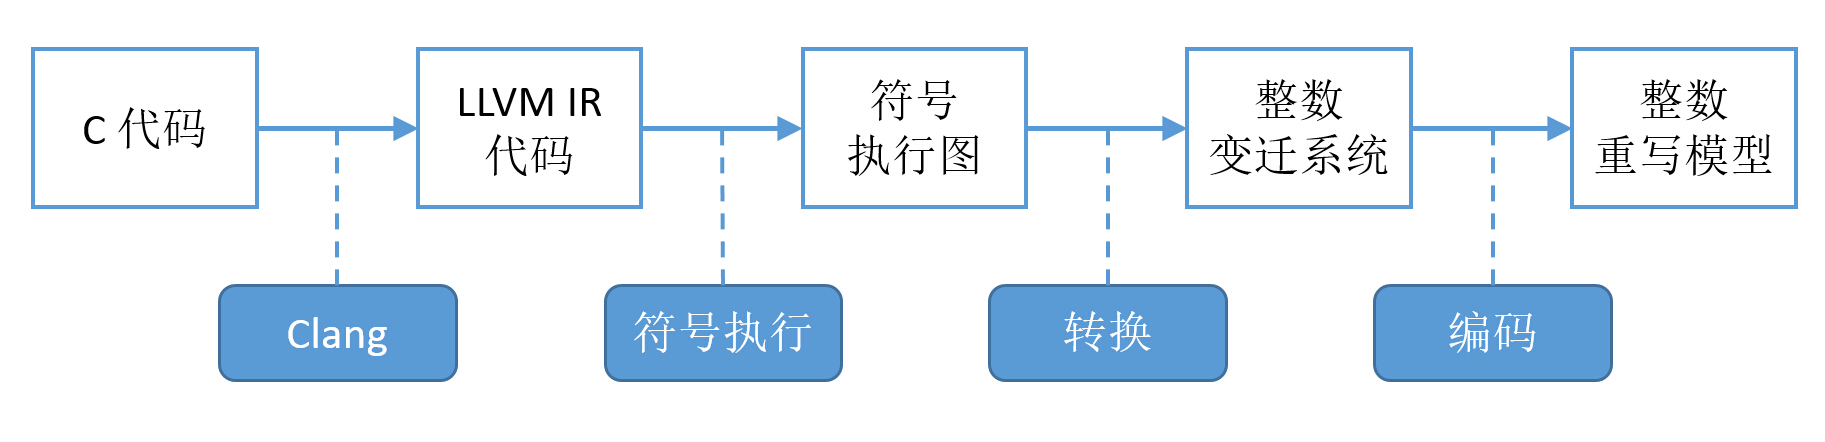
\includegraphics[width=\textwidth]{C2intTRS.jpg}
\caption{C 程序的整数重写模型自动构造}
\label{f:C2intTRS}
\end{figure}

图~\ref{f:C2intTRS} 是 C 程序的整数重写模型自动构造流程。C 程序经过编译器 Clang 的编译后生成对应的 LLVM IR~\cite{DBLP:conf/cgo/LattnerA04} 代码。基于这些 LLVM IR 代码,利用符号执行技术~\cite{DBLP:journals/cacm/King76},产生输入程序的符号执行图~\cite{DBLP:conf/lopstr/GieslSSEF12}。整数变迁系统~\cite{DBLP:journals/cacm/Keller76} 描述了该符号执行图的终止性行为。最后利用重写模型丰富的表达能力,将该整数变迁系统的语义编码成整数重写模型的形式。

这个构造过程涉及到三个重要的模型:符号执行图、整数变迁系统和整数重写模型。在本小节接下来的部分将对这三个概念进行介绍,并对其构造的核心原理进行描述。

\subsection{符号执行图}
\label{ss:seg}

\emph{符号执行图}(Symbolic execution graph)是由 Giesl 等人提出的用于描述程序执行过程的数据结构~\cite{DBLP:conf/lopstr/GieslSSEF12}。一个符号执行图是一个有向图,它包含一个顶点集合和一个边集合。每个顶点代表一个\emph{抽象}的程序执行状态,它包含程序当时的位置(pc)、变量赋值状态、内存分配情况等信息。程序执行图的边分为三类:
\begin{enumerate} [(i)]
\item 求值(Evaluation)类型。求值类型的边表示:若其起始顶点表示的程序状态为 $s$,当前程序位置为 $p$($p$ 也是状态 $s$ 中包含的信息),则 $s$ 在执行 $p$ 位置的程序指令后,其状态 $s'$ 为该有向边的终止顶点代表的状态。
\item 精化(Refinement)类型。精化类型的边的终止顶点 $v$ 所表示的状态是起始顶点 $u$ 表示的状态的精化,即 $v$ 所表示的程序状态集合是 $u$ 所表示的程序状态集合的子集。
\item 抽象(Abstraction)类型。抽象类型的边与精化类型的边相反,它表示其终止顶点 $v$ 的状态是起始顶点 $u$ 状态的抽象,即 $u$ 所表示的程序状态集合是 $v$ 所表示的程序状态集合的子集。
\end{enumerate}

至于每个顶点所表示的抽象程序状态,本文基于文献~\inlinecite{DBLP:conf/cade/StroderGBFFHS14} 的定义,进行了简化:
\begin{definition}[抽象程序状态] 
\label{d:abstract-state}
给定程序变量集合 $\VP$,符号化变量集合 $\Vsym$,程序位置集合 $Pos$,则一个抽象程序状态是一个六元组 $\lb p, LV, LAL, KB, AL, PT \rb$。其中 $p\in Pos$;$LV : \VP \ra \Vsym$;$LAL = \{\interp{v_1,v_2}\mid v_1,v_2\in\Vsym, v_1\le v_2 \}$;$KB\subseteq QF\_IA(\Vsym)$;$AL = \{\interp{v_1,v_2}\mid v_1,v_2\in\Vsym, v_1\le v_2 \}$;$PT \subseteq \{(v_1\pta_{\ty} v_2)\mid v_1,v_2\in\Vsym, \ty \mbox{是LLVM的类型}\}$。另外,抽象程序状态 $ERR$ 表示可能违背了内存安全的状态;抽象程序状态 $END$ 表示执行结束的程序状态。
\end{definition}

直观上解释,$LV$(Local variables)表示该状态的程序变量赋值情况,程序变量值由集合 $\Vsym$ 中的符号化变量表示;$LAL$(Local allocation list)表示局部内存分配情况,二元组 $\interp{v_1,v_2}$ 表示在 $v_1$ 和 $v_2$ 之间的内存单元是已经过分配的;$QF\_IA(\Vsym)$ 是指\emph{无量词的}(Quantifier-free)一阶公式,用于描述 $\Vsym$ 变量的\emph{整数代数}(Integer arithmetic)性质,$KB$(Knowledge base)是该状态满足的性质集合;$AL$(Allocation list)与 $LAL$ 类似,表示的是全局内存分配情况;$PT$(Pointer table)表示内存状态,元组 $(v_1\pta v_2)$ 表示内存地址 $v_1$ 指向的内容是 $v_2$,具有类型 $\ty$。

定义~\ref{d:abstract-state} 与文献~\inlinecite{DBLP:conf/cade/StroderGBFFHS14} 对抽象程序状态定义的最主要区别是,定义~\ref{d:abstract-state} 描述了单函数的抽象状态,而文献~\inlinecite{DBLP:conf/cade/StroderGBFFHS14} 的定义包含了栈结构,允许描述多函数之间的调用。

基于我们的简化定义,我们定义用于描述每个抽象程序状态的一阶谓词集合 $\lb a\rb$:
\begin{definition}[\inlinecite{DBLP:journals/jar/StroderGBFFHSA17}]
给定抽象程序状态 $a$,一阶谓词集合 $\lb a\rb$ 是满足以下条件的最小集合:
\begin{eqnarray}
\lb a \rb & = & KB 
\cup \{1\le v_1\land v_1\le v_2 
    \mid \interp{v_1, v_2} \in LAL \cup AL  \} \nonumber \\
& & \cup\; \{ v_2 < w_1 \lor w_2 < v_1 
    \mid \interp{v_1,v_2},\interp{w_1,w_2}\in LAL\cup AL, (v_1,v_2)\not= (w_1,w_2) \}    \nonumber \\
& & \cup\; \{ v_2 = w_2 \mid (v_1\pta_{\ty}v_2),(w_1\pta_{\ty}w_2)\in PT 
    \mbox{ and } \vDash \lb a\rb \Dra  v_1=w_1   \} \nonumber \\
& & \cup\; \{ v_1 \not= w_1 \mid (v_1\pta_{\ty}v_2),(w_1\pta_{\ty}w_2)\in PT 
    \mbox{ and } \vDash \lb a\rb \Dra  v_2\not=w_2   \} \nonumber \\
& & \cup\; \{ v_1 > 0 \mid (v_1\pta_{\ty} v_2) \in PT \} \;\;\mbox{。} \nonumber
\end{eqnarray}
\end{definition}

需要注意,$\lb a\rb$ 是归纳定义的。$\lb a \rb$ 定义了抽象程序状态 $a$ 满足的一阶谓词性质集合。

符号执行图的构建基于符号执行规则进行。给定一个抽象程序状态,根据符号执行规则计算下一个(或两个)抽象程序状态。由于实际的程序状态空间可能是无穷的,为了用符号执行图的有穷顶点数表示无穷的程序状态空间,在构造过程中需要根据一定的策略对抽象程序状态进行抽象。下面先介绍符号执行规则,再介绍符号执行图的构造策略。

基于定义~\ref{d:abstract-state},我们对文献~\inlinecite{DBLP:conf/cade/StroderGBFFHS14} 和~\inlinecite{DBLP:journals/jar/StroderGBFFHSA17} 的符号执行规则进行简化。以下列举其中较关键的几条符号执行规则。


\begin{table}[htbp]
\caption{符号执行规则:\texttt{load} 指令(内存已分配)}
\label{tab:rule-load-alloc}
\begin{tabularx}{\textwidth}{|X|}
\hline
\textbf{\texttt{load}} \emph{已分配内存} \\
{\centering $
\inferrule
   {\lb p, LV, LAL, KB, AL, PT\rb}
   {\lb p^+, LV[\texttt{x}:= w], LAL, KB, AL, PT\cup\{LV(\texttt{ad})\pta_{\ty} w \}\rb }
$ \\}
\textbf{如果满足以下条件} \\
~$\bullet$ $p$ : "\texttt{x = load ty* ad}" 其中 $\texttt{x},\texttt{ad}\in\VP$; \\
~$\bullet$ 存在 $\interp{v_1,v_2}\in LAL\cup AL$ \newline 
~\phantom{$\bullet$ } 使得 $\vDash \lb a\rb \Dra (v_1\le LV(\texttt{ad}) \land LV(\texttt{ad}) + size(\ty)-1\le v_2)$;  \\
~$\bullet$ $w\in\Vsym$ 是新变量。 \\
\hline
\end{tabularx}
\end{table}

\begin{table}[htbp]
\caption{符号执行规则:\texttt{load} 指令(内存未分配)}
\label{tab:rule-load-unalloc}
\begin{tabularx}{\textwidth}{|X|}
\hline
\textbf{\texttt{load}} \emph{未分配内存} \\
{\centering $
\inferrule
   {\lb p, LV, LAL, KB, AL, PT\rb}
   {ERR}
$ \\}
\textbf{如果满足以下条件} \\
~$\bullet$ $p$ : "\texttt{x = load ty* ad}" 其中 $\texttt{x},\texttt{ad}\in\VP$; \\
~$\bullet$ 不存在 $\interp{v_1,v_2}\in LAL\cup AL$ \newline 
~\phantom{$\bullet$ } 使得 $\vDash \lb a\rb \Dra (v_1\le LV(\texttt{ad}) \land LV(\texttt{ad}) + size(\ty)-1\le v_2)$。  \\
\hline
\end{tabularx}
\end{table}

表~\ref{tab:rule-load-alloc} 和~\ref{tab:rule-load-unalloc} 分别是 \verb|load| 指令从已分配内存和未分配内存中读取数据时对应的符号执行规则。如表~\ref{tab:rule-load-alloc} 所示,当 \verb|load| 指令准备从地址 \verb|ad| 中读取数据时,需要先判断是否能根据当前抽象程序状态 $a$ 的谓词表达式 $\lb a \rb$ 推断出地址 \verb|ad| 对应的内存块 $\interp{LV(\texttt{ad}), LV(\texttt{ad})+ size(\ty) -1}$ 已经经过分配。如果该内存块已经经过分配,则可执行表~\ref{tab:rule-load-alloc} 中的符号执行规则生成新的抽象程序状态,新状态中的程序变量 \verb|x| 得到更新,程序指针指向 $p$ 的下一条指令 $p^+$。如果不能推断出该内存块已经经过分配,则如表~\ref{tab:rule-load-unalloc} 所示,将产生抽象程序状态 $ERR$。

\begin{table}[htbp]
\caption{符号执行规则:\texttt{icmp eq} 指令(命题成立)}
\label{tab:rule-icmp-eq-true}
\begin{tabularx}{\textwidth}{|X|}
\hline
\textbf{\texttt{icmp eq}} \emph{命题为真} \\
{\centering $
\inferrule
   {\lb p, LV, LAL, KB, AL, PT\rb}
   {\lb p^+, LV[\texttt{x} := w], LAL, KB\cup\{w=1\}, AL, PT\rb}
$ \\}
\textbf{如果满足以下条件} \\
~$\bullet$ $p$ : "\texttt{x = icmp eq ty $t_1$, $t_2$}" 其中 $\texttt{x}\in\VP$ 且 $t_1,t_2\in\VP\cup\mathbb{Z}$; \\
~$\bullet$ $\vDash \lb a\rb \Dra (LV(t_1) = LV(t_2))$;  \\
~$\bullet$ $w\in\Vsym$ 是新变量。 \\
\hline
\end{tabularx}
\end{table}

\begin{table}[htbp]
\caption{符号执行规则:\texttt{icmp eq} 指令(命题不成立)}
\label{tab:rule-icmp-eq-false}
\begin{tabularx}{\textwidth}{|X|}
\hline
\textbf{\texttt{icmp eq}} \emph{命题为假} \\
{\centering $
\inferrule
   {\lb p, LV, LAL, KB, AL, PT\rb}
   {\lb p^+, LV[\texttt{x} := w], LAL, KB\cup\{w=0\}, AL, PT\rb}
$ \\}
\textbf{如果满足以下条件} \\
~$\bullet$ $p$ : "\texttt{x = icmp eq ty $t_1$, $t_2$}" 其中 $\texttt{x}\in\VP$ 且 $t_1,t_2\in\VP\cup\mathbb{Z}$; \\
~$\bullet$ $\vDash \lb a\rb \Dra (LV(t_1) \not= LV(t_2))$;  \\
~$\bullet$ $w\in\Vsym$ 是新变量。 \\
\hline
\end{tabularx}
\end{table}

表~\ref{tab:rule-icmp-eq-true} 和~\ref{tab:rule-icmp-eq-false} 是指令 \verb|icmp| 的符号执行规则。这里只列出了 \verb|icmp eq| 的具体规则,其它比较操作(如 \verb|ule|、\verb|uge| 等)的规则类似。如果当前状态的性质集合 $\lb a\rb$ 可以推断出 \verb|icmp eq| 指令对应命题为真,如表~\ref{tab:rule-icmp-eq-true} 所示,则下一状态将程序变量 \verb|x| 的值赋为 $w$,$KB$ 告诉我们 $w=1$。否则,如果 $\lb a\rb$ 足以推断出该命题为假,则 \verb|x| 对应的值为 0。
如果 $\lb a\rb$ 所包含的信息不能推断出目标命题的真假,这说明下一个状态需要分情况讨论。于是我们需要往当前的抽象程序状态加入更多的信息,对状态进行“精化”。

\begin{table}[htbp]
\caption{符号执行规则:精化(\texttt{icmp eq} 指令)}
\label{tab:rule-refine-icmp-eq}
\begin{tabularx}{\textwidth}{|X|}
\hline
\emph{对} \textbf{\texttt{icmp eq}} \emph{进行精化}  \\
{\centering $
\inferrule
   {\lb p, LV, LAL, KB, AL, PT\rb}
   {\lb p, LV, LAL, KB\cup\{\varphi\}, AL, PT\rb \;\;\mid\;\; \lb p, LV, LAL, KB\cup\{\lnot\varphi\}, AL, PT\rb}
$ \\}
\textbf{如果满足以下条件} \\
~$\bullet$ $p$ : "\texttt{x = icmp eq ty $t_1$, $t_2$}" 其中 $\texttt{x}\in\VP$ 且 $t_1,t_2\in\VP\cup\mathbb{Z}$; \\
~$\bullet$ $\not\vDash \lb a\rb \Dra \varphi$ 且 $\not\vDash \lb a\rb \Dra \lnot\varphi$; \\
~$\bullet$ $\varphi$ 是 $LV(t_1) \not= LV(t_2)$。 \\
\hline
\end{tabularx}
\end{table}

表~\ref{tab:rule-refine-icmp-eq} 是对指令 \verb|icmp eq| 进行精化的规则。若根据当前抽象状态的信息不能推断出命题 $\varphi$ 的真假,则精化规则产生两个新的抽象程序状态,两个状态的集合 $KB$ 分别加入了 $\varphi$ 的真假信息,使后续的状态求值可以继续进行。其它涉及条件比较的指令的精化规则,也可以类似地进行定义。

\begin{table}[htbp]
\caption{符号执行规则:\texttt{add} 指令}
\label{tab:rule-add}
\begin{tabularx}{\textwidth}{|X|}
\hline
\textbf{\texttt{add}} \\
{\centering $
\inferrule
   {\lb p, LV, LAL, KB, AL, PT\rb}
   {\lb p^+, LV[\texttt{x} := w], LAL, KB\cup\{w= LV(t_1) + LV(t_2)\}, AL, PT\rb} 
$ \\}
\textbf{如果满足以下条件} \\
~$\bullet$ $p$ : "\texttt{x = add ty $t_1$, $t_2$}" 其中 $\texttt{x}\in\VP$ 且 $t_1,t_2\in\VP\cup\mathbb{Z}$; \\
~$\bullet$ $w\in\Vsym$ 是新变量。 \\
\hline
\end{tabularx}
\end{table}

表~\ref{tab:rule-add} 展示了代数运算指令 \verb|add| 的符号执行规则。

\begin{table}[htbp]
\caption{符号执行规则:\texttt{alloca} 指令(分配错误)}
\label{tab:rule-alloca-err}
\begin{tabularx}{\textwidth}{|X|}
\hline
\textbf{\texttt{alloca}} \emph{失败} \\
{\centering $
\inferrule
   {\lb p, LV, LAL, KB, AL, PT\rb}
   {ERR} 
$ \\}
\textbf{如果满足以下条件} \\
~$\bullet$ $p$ : "\texttt{x = alloca ty, i$n$ $t$}" 其中 $\texttt{x}\in\VP$ 且 $t\in\VP\cup\mathbb{Z}$; \\
~$\bullet$ $\not\vDash \lb a\rb \Dra (LV(t) > 0)$。 \\
\hline
\end{tabularx}
\end{table}

\begin{table}[htbp]
\caption{符号执行规则:\texttt{alloca} 指令(分配成功)}
\label{tab:rule-alloca}
\begin{tabularx}{\textwidth}{|X|}
\hline
\textbf{\texttt{alloca}} \emph{成功} \\
{\centering $
\inferrule
   {\lb p, LV, LAL, KB, AL, PT\rb}
   {\lb p^+, LV[\texttt{x} := v_1], LAL\cup\{\interp{v_1,v_2}\}, KB\cup\{v_2= v_1 + size(\ty)\cdot LV(t)-1\}, AL, PT\rb} 
$ \\}
\textbf{如果满足以下条件} \\
~$\bullet$ $p$ : "\texttt{x = alloca ty, i$n$ $t$}" 其中 $\texttt{x}\in\VP$ 且 $t\in\VP\cup\mathbb{Z}$; \\
~$\bullet$ $\vDash \lb a\rb \Dra (LV(t) > 0)$; \\
~$\bullet$ $v_1,v_2\in\Vsym$ 是新变量。 \\
\hline
\end{tabularx}
\end{table}

表~\ref{tab:rule-alloca-err} 和~\ref{tab:rule-alloca} 是 \verb|alloca| 指令的符号执行规则。分配内存成功的前提是,当前状态信息足以推断出分配的内存块大小为正数,否则则产生错误状态 $ERR$(如表~\ref{tab:rule-alloca-err})。当分配内存成功时,新状态的主要变化是其局部内存分配表 $LAL$ 中增加了一块新的内存区域 $\interp{v_1,v_2}$。符号变量 $v_1$ 与 $v_2$ 的关系在性质集合 $KB$ 中体现。


\begin{table}[htbp]
\caption{符号执行规则:\texttt{call} 指令}
\label{tab:rule-call}
\begin{tabularx}{\textwidth}{|X|}
\hline
\textbf{\texttt{call}} \\
{\centering $
\inferrule
   {\lb p, LV, LAL, KB, AL, PT\rb}
   {\lb p^+, LV[\texttt{x} := w], LAL, KB, AL, PT\rb} 
$ \\}
\textbf{如果满足以下条件} \\
~$\bullet$ $p$ : "\texttt{x = call ty $\ldots$}" 其中 $\texttt{x}\in\VP$;\\
~$\bullet$ $w\in\Vsym$ 是新变量。 \\
\hline
\end{tabularx}
\end{table}

\begin{table}[htbp]
\caption{符号执行规则:\texttt{ret} 指令}
\label{tab:rule-ret}
\begin{tabularx}{\textwidth}{|X|}
\hline
\textbf{\texttt{ret}} \\
{\centering $
\inferrule
   {\lb p, LV, LAL, KB, AL, PT\rb}
   {END}
$ \\}
\textbf{如果满足以下条件} \\
~$\bullet$ $p$ : "\texttt{ret ty $t$}" 其中 $t\in\VP\cup\mathbb{Z}$。\\
\hline
\end{tabularx}
\end{table}

表~\ref{tab:rule-call} 和~\ref{tab:rule-ret} 分别是 \verb|call| 指令和 \verb|ret| 指令的符号执行规则。由于本文采用单函数分析的方法,因此对 \verb|call| 指令与 \verb|ret| 指令的处理比文献~\inlinecite{DBLP:conf/cade/StroderGBFFHS14} 和~\inlinecite{DBLP:journals/jar/StroderGBFFHSA17} 精简。应用 \verb|call| 指令时,由于我们对所有函数逐一进行终止性分析,因此可以假设被 \verb|call| 调用的函数将返回某值。于是表~\ref{tab:rule-call} 的执行规则中,变量 \verb|x| 被赋予新的未知值。在程序中遇到 \verb|ret| 指令时,由于是单函数分析,如表~\ref{tab:rule-ret} 所示,下一状态为结束状态 $END$。

\begin{table}[htbp]
\caption{符号执行规则:抽象}
\label{tab:rule-abstract}
\begin{tabularx}{\textwidth}{|X|}
\hline
\emph{利用代换 $\mu$ 进行抽象} \\
{\centering $
\inferrule
   {\lb p, LV, LAL, KB, AL, PT\rb}
   {\lb p, LV', LAL', KB', AL', PT'\rb }
$ \\}
\textbf{如果满足以下条件} \\
~$\bullet$ $a$ 有一条求值类型的入边; \\
~$\bullet$ $LV$ 和 $LV'$ 的域相同,而且对所有 $\texttt{x} \in\VP$ 满足 $LV(\texttt{x}) = \mu(LV'(\texttt{x}))$; \\
~$\bullet$ $\vDash \lb a\rb \Dra \mu(KB')$;\\
~$\bullet$ 如果 $\interp{v_1,v_2}\in LAL'$,那么 $\interp{\mu(v_1),\mu(v_2)}\in LAL$; \\
~$\bullet$ 如果 $\interp{v_1,v_2}\in AL'$,那么 $\interp{\mu(v_1),\mu(v_2)}\in AL$; \\
~$\bullet$ 如果 $(v_1\pta_{\ty} v_2)\in PT'$,那么 $(\mu(v_1)\pta_{\ty}\mu(v_2))\in PT$。 \\
\hline
\end{tabularx}
\end{table}

最后是对抽象程序状态的抽象规则,如表~\ref{tab:rule-abstract} 所示。抽象后的新状态拥有同样的程序位置,新状态的信息可由原状态 $a$ 的一阶谓词集合推出。

有了符号执行规则,我们根据以下策略构造符号执行图~\cite{DBLP:conf/cade/StroderGBFFHS14,DBLP:journals/jar/StroderGBFFHSA17}:
\begin{itemize}
\item 
假设当前需要应用符号执行规则的状态顶点为 $b$,如果存在某个状态顶点 $a$ 满足:(i) 存在从 $a$ 到 $b$ 的一条路径;(ii) $a$ 和 $b$ 的程序位置 $p$ 相同;(iii) $a$ 和 $b$ 的 $LV$ 映射域相同;(iv) $b$ 存在一条求值类型的入边;(v) $a$ 不存在精化类型的入边。那么
\begin{itemize}
\item 如果状态 $a$ 是状态 $b$ 的抽象,那么构造一条抽象类型的边从 $b$ 指向 $a$。
\item 否则,移除 $a$ 的后继顶点,计算 $a$ 和 $b$ 的抽象 $c$ 并构造一条抽象类型的边从 $a$ 指向 $c$。如果 $a$ 已经存在来自某顶点 $q$ 的抽象类型入边,则将 $a$ 删除并构造一条抽象类型的边从 $q$ 指向 $c$。
\end{itemize}
\item
否则,对 $b$ 应用除抽象规则以外的符号执行规则,构造其后继顶点。
\end{itemize}

\subsection{整数变迁系统}

\begin{definition}[整数变迁系统~\cite{DBLP:journals/cacm/Keller76}]
整数变迁系统是一个三元组 $\lb S, C, \transto \rb$:
\begin{itemize}
\item $S$ 是一组状态集合 $\{s_1,\ldots,s_n\}$;
\item $C$ 是一组条件集合 $\{c_1,\ldots,c_m\}$;
\item ${\transto} \subseteq S \times C \times S$ 是一组变迁集合。
\end{itemize}
其中,条件 $c_i \subseteq QF\_IA(\cV\cup\cV')$ 是一组一阶公式,$\cV$ 是整数类型的变量集合,$\cV' = \{v' \mid v\in\cV \}$ 表示经过变迁后的变量值。
\end{definition}

整数变迁系统可以抽象地表示一个程序的状态空间和状态变迁。给定一个符号执行图,可以根据以下策略构造其对应的整数变迁系统~\cite{DBLP:conf/cade/StroderGBFFHS14,DBLP:journals/jar/StroderGBFFHSA17}:
\begin{enumerate} [(i)]
\item 符号执行图中每一个顶点 $a$ 都对应到整数变迁系统的一个状态 $s_a$;
\item 为符号执行图每一条从 $a$ 到 $b$ 的边构造一条对应的整数变迁系统的变迁 $\lb s_a, c, s_b\rb$:
\begin{itemize}
\item 如果 $\lb a, b\rb$ 不是一条抽象类型的边,则条件 $c = (\lb a\rb \cup \{v' = v | v\in\Vsym(a)\})$,其中 $\Vsym(a)$ 表示状态 $a$ 的所有符号化变量;
\item 如果 $\lb a, b\rb$ 是一条利用代换 $\mu$ 的抽象类型边,则条件 $c = (\lb a\rb \cup \{v'=\mu(v) \mid v\in\Vsym(b)\})$。
\end{itemize}
\end{enumerate}

\subsection{整数重写模型}
整数重写模型~\cite{DBLP:conf/rta/FalkeKS11} 是规范化条件重写模型 $\RSE = \lb \cR,\cS,\cE \rb$ 的一种实例。当等价模型 $\cE$ 取整数代数运算符的性质集合(如加法交换律、乘法结合律等),化简模型 $\cS$ 取整数代数的计算规则时,规范化条件重写模型 $\RSE$ 实例化为整数重写模型,记作 $\cR_{\cI}$。

整数重写模型的重写规则通常具有如下形式:
\begin{eqnarray}
f(x_1,\ldots,x_n) & \ra & g(e_1,\ldots,e_m) \;\Dla\; \varphi \nonumber
\end{eqnarray}
其中,$e_1,\ldots,e_m$ 为整数代数表达式,$\varphi\in QF\_IA(\cV)$。

给定一个整数变迁系统,系统中的每一条变迁 $\lb s_i, c, s_j \rb$ 都可以用一条重写规则进行编码~\cite{DBLP:conf/cade/FalkeK09,DBLP:conf/rta/FalkeKS11}:
\begin{eqnarray}
s_i(x_1,\ldots,x_n) & \ra & s_j(e_1,\dots,e_n) \;\Dla\; \varphi_c \nonumber
\end{eqnarray}
其中,$x_1,\ldots,x_n$ 按 $\cV$ 中变量的固定序排列,且
\begin{itemize}
\item 如果 $c$ 中包含“赋值语句” $x_i' = p$,则 $e_i = p$;否则 $e_i = x_i$。
\item $\varphi_c$ 是 $c$ 中除去“赋值语句”后的所有一阶公式的合取。
\end{itemize}

\section{\CTerm}
\label{s:ceagle-termination}

\subsection{工具组成}

\begin{figure}[ht]
\centering
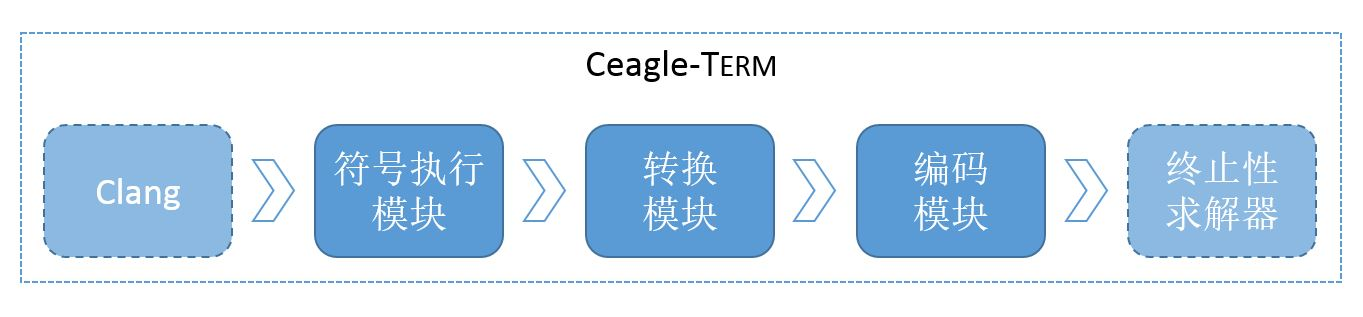
\includegraphics[width=\textwidth]{Ceagle-Termination.jpg}
\caption{\CTerm 组成}
\label{f:Ceagle-Termination}
\end{figure}

如图~\ref{f:Ceagle-Termination} 所示, \CTerm 主要由三部分构成:符号执行模块,转换模块和编码模块。前端接入第三方工具 Clang,将待验证的 C 程序编译成为 LLVM IR 程序。符号执行模块接受 LLVM IR 代码输入,生成对应的符号执行图。符号执行图经过转换模块后,输出整数变迁系统。该变迁系统经过编码模块的编码,生成适合后端重写模型终止性求解器的整数重写模型。后端接入第三方终止性求解器(目前支持开源求解器 \verb|KITTeL|~\cite{DBLP:conf/rta/FalkeKS11}),求解输出终止性验证结果。


\begin{algorithm}[htbp]
  \KwIn{$G$:只包含初始状态顶点的符号执行图}
  \KwIn{$path$:存放顶点的栈结构,初始状态只包含初始顶点}
  \KwOut{$G$:构建完成的符号执行图}

  \While{ $path$ 非空 }{
    $v = peek(path)$\;
    \uIf{$v.visited == false$}{
      
      \If(\tcp*[h]{如果 $v$ 是结束状态}){$v == END$} {
        $v.visited = true$; \qquad $path.pop()$\;
        continue\;
      }

      %\tcp{decide whether we should generalize}
      在 $path$ 中寻找程序位置与 $v$ 相同的顶点,组成列表 $list_v$ \;
      %$list = path.findSamePC(v)$\;
      $should = false$ \tcp*{判断是否应该进行抽象}

      \ForEach{$u\in list_v$}{
        \If{ $u$ 和 $v$ 满足应该抽象的判断条件 }{
            %$u.domain() == v.domain()$ \\
            %$\land$ $v$ has an incoming evaluation edge \\
            %$\land$ $u$ has no incoming refinement edge}{
          $should = true$; \qquad $target = u$\;
          break\;
        }
      }

      %\tcp{Now we know what we should do}
      \uIf{should}{
        %\tcc{Do generalization}
        %perform Algorithm~\ref{a:generalization}\;
        应用算法~\ref{alg:abstraction} 进行抽象\;
      } \Else {
        %\tcc{Do evaluation}
        %perform Algorithm~\ref{a:evaluation}\;
        应用算法~\ref{alg:evaluation} 进行符号执行\;
      }
    } \Else(\tcp*[h]{ $v$ 已被访问过}) {
      在 $G$ 中寻找一个未被访问的 $v$ 的后继顶点 $w$\;
      \uIf{ $w$ 不存在} {
        $pop(path)$\tcp*{将 $v$ 从栈中取出}
      } \Else {
        $push(w,path)$\;
      }
    }
  }
\caption{构建符号执行图}
\label{alg:seg}
\end{algorithm}

\begin{algorithm}[htbp]
\KwIn{$G$:正在构建的符号执行图 }
\KwIn{$v$:正在访问的顶点 }
\KwIn{$target$:$v$ 的抽象目标顶点 } 
\KwIn{$path$:当前搜索路径}
\KwOut{$G$, $path$}
  \uIf{ 状态 $target$ 是 $v$ 的抽象 }{
    $v.visited = true$\;
    %$G.add\_edge(v,genTarget,generalization)$\;
    在 $G$ 中添加从 $v$ 到 $target$ 的一条抽象类型的边\;
    $pop(path)$\tcp*{将 $v$ 从栈中取出}
  } \Else(\tcp*[h]{ 需要计算 $v$ 和 $target$ 的抽象 }) { 
    %$path.popupto(genTarget)$\;
    对 $path$ 进行出栈操作,直到 $target$ 成为栈顶元素\;
    %$G.removeChild(genTarget)$\;
    在 $G$ 中删除 $target$ 的后继顶点\;
    %$c = merge(v, genTarget)$\;
    %$G.add\_vertex(c)$\;
    计算 $v$ 和 $target$ 的抽象状态 $c$,并将其加入 $G$\;

    \uIf{ 如果 $path$ 中只含 $target$ 一个元素 } {
      %$G.add\_edge(genTarget,c,generalization)$\;
      在 $G$ 中添加从 $target$ 到 $c$ 的一条抽象类型的边\;
      $push(c,path)$\;
    } \Else {
      $pop(path)$\tcp*{将 $target$ 从栈中取出}
      $p = peek(path)$\;
      \uIf{ 在 $G$ 中存在从 $p$ 到 $target$ 的抽象类型的边 }{
        从 $G$ 中删除顶点 $target$ 及其边\;
        在 $G$ 中添加从 $p$ 到 $c$ 的一条抽象类型的边\;
        $push(c,path)$\;
      } \Else {
        在 $G$ 中添加从 $target$ 到 $c$ 的一条抽象类型的边\;
        $push(target,path)$\;
        $push(c,path)$\;
      }
    }
  }
\caption{状态抽象}
\label{alg:abstraction}
\end{algorithm}

\begin{algorithm}[htbp]
\KwIn{$G$:正在构建的符号执行图 }
\KwIn{$v$:正在访问的顶点 }
\KwIn{$path$:当前搜索路径}
\KwOut{$G$, $path$}
  $v.visited = true$\;
  %$stateList = v.evaluate()$\;
  对状态 $v$ 应用除抽象外的符号执行规则,获得新状态列表 $list_{new}$\;
  \uIf(\tcp*[h]{没有对 $v$ 应用精化规则 }){$size(list_{new}) == 1$ } {
    $w = list_{new}[0]$\;
    在 $G$ 中添加顶点 $w$ 以及从 $v$ 到 $w$ 的一条求值类型的边\;
    $push(w,path)$\;
  } \Else(\tcp*[h]{ 精化规则被应用,产生2个新状态 }) {
    $w_1 = list_{new}[0]$\;
    $w_2 = list_{new}[1]$\;
    在 $G$ 中添加顶点 $w_1$ 以及从 $v$ 到 $w_1$ 的一条求值类型的边\;
    在 $G$ 中添加顶点 $w_2$ 以及从 $v$ 到 $w_2$ 的一条求值类型的边\;
    $push(w_1,path)$\;
  }
\caption{求值与精化}
\label{alg:evaluation}
\end{algorithm}

\CTerm 的核心模块为符号执行模块,它涉及到对每一个抽象程序状态的符号执行、计算两个状态的抽象状态、以及对整个符号执行图进行构建。对状态的符号执行与抽象计算已经在小节\ref{ss:seg} 进行介绍,在此不再赘述。下面给出构建符号执行图的核心算法,见算法~\ref{alg:seg}。 

\subsection{性能评估} 
\todo{需要等到工具原型开发完成}
 
\todo{与 AProVE 、\texttt{KITTeL}、Ctrl 进行比较} 

\subsection{可扩展性}

由于 \CTerm 的核心模块——符号执行模块是针对 LLVM IR 实现的,得益于 LLVM 一般化的框架及丰富的工具集,通过接入不同的前端,\CTerm 可以支持更多类型的程序终止性验证。比如利用 GCC 搭配 DragonEgg~\cite{dragonegg} 作为前端,则可以实现对 Ada 语言~\cite{DBLP:journals/computer/WolfeBSTW81} 和 Fortran 语言~\cite{DBLP:books/sp/ChiversS15} 程序的终止性验证。

从后端的角度看,由于 \CTerm 输出的模型及模型格式由编码模块决定,因此通过对编码模块进行扩展,可以实现后端对更多重写模型终止性求解器的支持,比如 Ctrl~\cite{DBLP:conf/lpar/Kop015} 和 \TTT~\cite{DBLP:conf/rta/KorpSZM09}。 


\section{本章小结}

整数重写模型是规范化条件重写模型的一种特例。基于整数重写模型和符号执行图,我们开发了针对 C 语言程序终止性的自动验证工具 \CTerm。该工具接受 C 语言程序输入,并自动对其进行模型转换与终止性求解,不需要人工参与。

\todo{评价其表现}

\chapter{结束语}
\label{cha:conclusion}

\section{工作总结}

针对现代嵌入式系统结构复杂、行为复杂所引发的形式化建模与验证问题,本文基于重写理论,完成了以下工作:

\begin{enumerate}
\item 
针对嵌入式系统中硬件的并发行为与软件的顺序行为并存的异构性特征进行研究,提出了规范化条件重写模型。将硬件的并发行为抽象成不确定性行为,将软件的顺序行为抽象成确定性行为,基于模重写模型、条件重写模型以及 Nipkow 在高阶重写中使用的 $\beta\eta$ 规范化过程,本文提出的规范化条件重写模型,利用等式规则描述系统的结构特征及状态等价关系,利用条件约束描述系统的控制流特征,利用化简规则描述系统的确定性行为,利用重写规则描述系统的不确定性行为。本文对重写模型的规则应用策略进行扩展,定义了在多种规则共存的情况下,确定性行为与不确定性行为的协作方式,且保证了重写规则触发时条件约束的可判定性。规范化条件重写模型具有严格的形式化语法及语义定义。该模型是面向建模与验证的重写模型扩展,相比其它重写模型扩展,它的表达能力得到了提升。

\item
基于规范化条件重写模型,以嵌入式系统建模方法论为切入点就重写模型易用性低的问题进行研究。本文提出对嵌入式系统的结构层次性、行为异构性、结构动态性和实时性等特征的具体建模方法,对建模过程进行指导。基于语义映射的方式,将该建模方法在工具 Maude 中进行实现。通过对两个真实嵌入式系统的建模验证过程进行应用,验证了该建模方法在嵌入式系统中实际应用的可行性。其中,机车优化控制系统在本文的建模与验证过程中,成功发现了测试人员进行仿真测试未能发现的系统缺陷;该系统目前运行稳定,满足了铁路节能驾驶使用要求,并在沈阳铁路局通过了实车运用考核。速率单调调度系统的可调度性和正确性通过模型检测方法得到了验证,且本文证明了该结果具有可靠性和完备性;该调度系统目前在某工业级航天控制器中在线运行。

\item 
基于整数重写模型这一规范化条件重写模型实例,针对重写模型易用性低的问题,以嵌入式系统软件的自动建模为切入点进行研究。本文设计、开发了一套针对 C 语言程序终止性的自动验证工具 \CTerm。为增加工具的可扩展性,\CTerm 采用 LLVM IR 作为程序的中间表示语言。参考已有工具,\CTerm 采用符号执行技术生成符号执行图作为程序行为的中间模型。它的后端可以接入多种重写模型终止性求解器,进一步提高了它的可扩展性。\CTerm 接受 C 语言程序输入,并自动得到终止性验证结果,有效降低了形式化验证方法的使用成本。
\end{enumerate}

\section{研究展望}

在本文的工作基础上,为了进一步推动规范化条件重写模型在嵌入式系统建模与验证工作中的应用,拟在以下方面开展更多研究工作:

\begin{enumerate}
\item 
对条件模重写模型的终止性与合流性研究。在规范化条件重写模型 $\lb \cR,\cS,\cE\rb$ 的定义中,要求 $\cS$ 和 $\cE$ 使条件模重写模型 $\SE$ 满足终止性和合流性。从建模的角度看,根据第~\ref{s:modeling} 小节提出的建模方法,$\cS$ 用于建模系统的确定性行为(如软件的局部顺序行为),$\cE$ 用于描述项表达式的结构信息,因此 $\SE$ 的终止性和合流性可以由建模的方法得到保证。然而建模过程是由人主导的,人总是容易出错,这正是为什么需要对系统进行验证的原因。从理论和工具的角度对 $\SE$ 的终止性和合流性进行检查,不但可以保证模型的一致性(consistency),还可以发现建模过程引入的错误。虽然目前存在对模重写模型的终止性和合流性的研究\cite{DBLP:conf/cade/JouannaudM84,DBLP:journals/tcs/JouannaudM92,DBLP:journals/ijsi/JouannaudT08,DBLP:conf/rta/Jouannaud06,DBLP:journals/tcs/JouannaudL12,DBLP:journals/siamcomp/JouannaudK86},但目前的结果对等价模型 $\cE$ 具有较严格的约束。因此,要推动规范化条件重写模型在建模过程中的应用,需要对模重写模型的终止性和合流性进行更一般化的理论研究,以及相应检查工具的开发。
\item
进一步提高和完善基于规范化条件重写模型的建模方法。现代嵌入式系统种类繁多、行为复杂,需要在更多实际案例上应用本文提出的基于规范化条件重写模型的建模方法,发现它在应对不同系统时产生的问题,对其进行进一步提高和完善。对该建模方法的另一个可行的完善方式,是针对不同的特定的嵌入式系统,如中断系统、调度系统等,设计领域特定语言(Domain Specific Language,DSL)来对特定系统进行建模,并将 DSL 模型翻译成对应的规范化条件重写模型。
\item 
完善规范化条件重写模型建模的支持工具集。如第~\ref{ss:method-impl} 小节所述,工具 Maude 不能完全支持规范化条件重写模型的建模,其根本原因在于 Maude 的理论模型——重写逻辑的表达能力不如规范化条件重写模型。因此,对 Maude 的底层核心模块进行扩展,或开发专门针对规范化条件重写模型的建模验证工具集,可以更充分地发挥规范化条件重写模型的作用。
\item 
提高和完善 \CTerm 工具。一方面,由于 \CTerm 采用符号执行技术对模型进行构建,这导致在大规模程序上进行应用时要耗费大量的计算资源。因此,为了降低模型构建的资源占用问题,也为了减小模型规模,可以考虑使用诸如切片~\cite{DBLP:journals/tse/Weiser84} 等程序分析变形技术,在构建模型前对程序中与终止性无关的代码进行削减。另一方面,在构造程序的符号执行图时,抽象规则会导致状态的信息丢失。而在丢失的状态信息中,可能存在某些对终止性判定有用的信息,比如循环不变式~\cite{DBLP:journals/cacm/Hoare69}。设计新的抽象规则,使更多的有用信息得到保留,同时尽量减少不必要的信息,是一个值得研究的方向。再者,虽然目前的内存模型以及对函数调用的执行规则可以保证符号执行图的构造过程在递归函数存在时得以终止,但这并没有完全解决对递归函数的建模问题。如何对递归函数的语义进行精确建模,这是一个从理论和应用层面都值得研究的问题。最后,将不同的终止性验证技术进行融合,是完善 \CTerm 工具的另一个方向。
\end{enumerate}

%%% 其它部分
\backmatter

%% 本科生要这几个索引,研究生不要。选择性留下。
% 插图索引
%%\listoffigures
% 表格索引
%%\listoftables
% 公式索引
%%\listofequations


%% 参考文献
% 注意:至少需要引用一篇参考文献,否则下面两行可能引起编译错误。
% 如果不需要参考文献,请将下面两行删除或注释掉。
\bibliographystyle{thuthesis}
\bibliography{ref/refs}


%% 致谢
% 如果使用声明扫描页,将可选参数指定为扫描后的 PDF 文件名,例如:
% \begin{acknowledgement}[scan-statement.pdf]
\begin{acknowledgement}

\hide{
  衷心感谢导师 xxx 教授和物理系 xxx 副教授对本人的精心指导。他们的言传身教将使
  我终生受益。

  在美国麻省理工学院化学系进行九个月的合作研究期间,承蒙 xxx 教授热心指导与帮助,不
  胜感激。感谢 xx 实验室主任 xx 教授,以及实验室全体老师和同学们的热情帮助和支
  持!本课题承蒙国家自然科学基金资助,特此致谢。

  感谢 \thuthesis,它的存在让我的论文写作轻松自在了许多,让我的论文格式规整漂亮了
  许多。}
\end{acknowledgement}
 

%% 附录
\begin{appendix}
\chapter{定理~\ref{t:main} 的证明}
\label{app:proof}

本附录给出定理~\ref{t:main} 的详细证明。

为了证明定理~\ref{t:main},我们需要先介绍更多关于重写逻辑的背景知识~\cite{DBLP:journals/entcs/OlveczkyM07a}。如果一个项表达式 $t$ 不含变量,那么 $t$ 称作是\emph{封闭的}(ground)。给定原子命题的一个子集 $P\subseteq AP$ 和封闭的项表达式 $t$ 和 $t'$,如果 $t$ 满足的 $P$ 中的命题和 $t'$ 所满足的 $P$ 的命题完全一致,则记作 $t\simeq_P t'$ (如果 $P$ 可从上下文推断,则简记为 $t\simeq t'$)。

时间鲁棒性是我们希望一个实时重写逻辑模型所具有的一系列性质的集合。为了简化概念,我们在这里避免给出时间鲁棒性的准确定义,因为它对本附录的证明无关重要。我们给出以下引理用于证明时间鲁棒性:
\begin{lemma}[\inlinecite{DBLP:journals/entcs/OlveczkyM07a}]
\label{l:timerobustness}
给定一个面向对象风格的模型 $\mathcal{R^L}$,它只包含一条标准的单元计时规则,且满足时间域中只包含一个非正常的时间值为 \verb|INF|。如果 $\mathcal{R^L}$ 对所有封闭的项表达式 $t$、$r$ 和 $r'$ 满足以下条件,则 $\mathcal{R^L}$ 具有时间鲁棒性:
\begin{enumerate}[(i)]
\item 
对所有 $r\le$ \verb|mte(|$t$\verb|)| 满足 \verb|mte(delta(|$t$\verb|,|$r$\verb|))| $=$ \verb|mte(|$t$\verb|) monus |$r$,其中 \verb|monus| 是内置类型 \verb|Time| 的减法操作;

\item
\verb|delta(|$t$\verb|,|$0$\verb|)| $= t$;

\item
对所有 $r+r'\le$ \verb|mte(|$t$\verb|)| 满足 \verb|delta(delta(|$t$\verb|,|$r$\verb|),|$r'$\verb|)| $=$ \verb|delta(|$t$\verb|,|$r+r'$\verb|)|;

\item
对任意瞬时重写规则的左项表达式 $l$ 的所有封闭实例 $\sigma(l)$ 满足 \verb|mte(|$\sigma(l)$\verb|)|$= 0$。
\end{enumerate}
\end{lemma}

任意一步重写可以被分类,在此基础上,我们可以定义单元计时不变性。
\begin{definition}[\inlinecite{DBLP:journals/entcs/OlveczkyM07a}]
给定重写步骤 $t\lrps{r}{}t'$,假定它应用了单元计时规则,且其上标 $r$ 代表该重写的时间推移为 $r$:
\begin{itemize}
\item 
如果不存在时间值 $r'>r$ 使得对于某个 $t''$ 满足 $t\lrps{r'}{}t''$,则该重写步骤被称为一个\emph{极大的单元计时步骤}(maximal tick step),记作 $t\lrps{r}{max}t'$;

\item 
如果对任意时间值 $r'>0$,都存在某个 $t''$ 满足 $t\lrps{r'}{}t''$,则该重写步骤被称作一个 \emph{$\infty$ 单元计时步骤}($\infty$ tick step),记作 $t\lrps{r}{\infty}t'$;

\item 
如果存在一个极大的单元计时步骤 $t\lrps{r'}{max}t''$ 满足 $r'>r$,则该重写步骤被称为一个\emph{非极大的单元计时步骤}(non-maximal tick step)。
\end{itemize}
\end{definition}

\begin{definition}[\inlinecite{DBLP:journals/entcs/OlveczkyM07a}]
一个时间鲁棒的模型 $\mathcal{R^L}$ 被称作根据一个命题集合 $P$ 保持单元计时不变,当且仅当,对任意非极大的单元计时步骤或 $\infty$ 单元计时步骤 $t\lrps{r}{}t'$ 有 $t\simeq_P t'$ 成立。
\end{definition}

我们需要以下引理证明我们的模型根据我们定义的命题具有单元计时不变性:
\begin{lemma}[\inlinecite{DBLP:journals/entcs/OlveczkyM07a}]
\label{l:tickinv}
给定一个时间鲁棒的、面向对象风格的模型 $\mathcal{R^L}$,它只包含一条标准的单元计时规则,且满足时间域中只包含一个非正常的时间值为 \verb|INF|。如果对于所有满足 $r<$ \verb|mte(|$t$\verb|)| 的 $t$ 和 $r$,都有 \verb|{|$t$\verb|}| $\simeq_P$ \verb|{delta(|$t$\verb|,|$r$\verb|)}| 成立,那么 $\mathcal{R^L}$ 是根据原子命题集合 $P$ 保持单元计时不变的。
\end{lemma}

\newcommand{\mteTask}[2]{\texttt{mteTask(}#1\texttt{,}#2\texttt{)}}
\newcommand{\deltaTask}[3]{\texttt{deltaTask(}#1\texttt{,}#2\texttt{,}#3\texttt{)}}
\newcommand{\mteIS}[1]{\texttt{mteIS(}#1\texttt{)}}
\newcommand{\deltaIS}[2]{\texttt{deltaIS(}#1\texttt{,}#2\texttt{)}}
\newcommand{\IntSrc}[3]{\texttt{<}#1\texttt{:IntSrc|val:}#2\texttt{,cycle:}#3\texttt{>}}
\newcommand{\mteIr}[1]{\texttt{mteIr(}#1\texttt{)}}
\newcommand{\mteS}[1]{\texttt{mte(}#1\texttt{)}}
\newcommand{\deltaS}[2]{\texttt{delta(}#1\texttt{,}#2\texttt{)}}
 
我们先证明以下中间引理:
\begin{lemma}
\label{l:auxtask}
给定分别具有类型 \verb|MaybeNat| 和 \verb|TaskList| 的项表达式 $\mathit{ID}$ 和 $L$,对所有 $r\le\mteTask{\mathit{ID}}{L}$,有 $\mteTask{\mathit{ID}}{\deltaTask{\mathit{ID}}{L}{r}} = \mteTask{\mathit{ID}}{L}\; \verb|monus|\;r$ 成立。
\end{lemma}
\begin{proof}
如果 $\mathit{ID}=\verb|none|$,则此情况显而易见。根据定义,有
\begin{eqnarray*}
& & \mteTask{\texttt{none}}{\deltaTask{\texttt{none}}{L}{r}} \\
& = & \mteTask{\texttt{none}}{L} \\
& = & \verb|INF| \\
& = & \mteTask{\texttt{none}}{L}~\verb|monus|~r \;\;\;\mbox{。}
\end{eqnarray*}

否则,存在具有类型 \verb|Nat| 的项表达式 $N$,使 $\mathit{ID}= \verb|some|~N$。假设 $L$ 的第 $N$ 个任务的 \verb|cnt| 值为 \verb|[|$r_e$\verb|/|$C$\verb|]|。则根据定义,$\deltaTask{\mathit{ID}}{L}{r}=L'$ 成立,其中 $L'$ 的第 $N$ 个任务的 \verb|cnt| 值等于 \verb|[|$(r_e+r)$\verb|/|$C$\verb|]|。因此,
\begin{eqnarray*}
& & \mteTask{\mathit{ID}}{\deltaTask{\mathit{ID}}{L}{r}} \\  
& = & \mteTask{\mathit{ID}}{L'} \\
& = & C~\verb|monus|~(r_e+r) \\
& = & (C~\verb|monus|~r_e)~\verb|monus|~r \\
& = & \mteTask{\mathit{ID}}{L}~\verb|monus|~r\;\;\;\mbox{。}
\end{eqnarray*}

以上,引理得证。
\end{proof}

\begin{lemma}
\label{l:auxis}
给定具有类型 \verb|IntSrc| 的项表达式 $\mathit{ISRC}$,它表示我们的模型中中断源的一个可达状态。则对所有 $r\le\mteIS{\mathit{ISRC}}$,$\mteIS{\deltaIS{\mathit{ISRC}}{r}} = \mteIS{\mathit{ISRC}}\;\verb|monus|~r$ 成立。
\end{lemma}
\begin{proof}
任意可达状态 $\mathit{ISRC}$ 必然具有以下形式 $\IntSrc{O}{v}{T}$,其中 $v\le T$。因此,
\begin{eqnarray*}
&  & \mteIS{\deltaIS{\mathit{ISRC}}{r}} \\  
& = & \mteIS{\IntSrc{O}{(v~\texttt{monus}~r)}{T}} \\
& = & v~\texttt{monus}~r \\
& = & \mteIS{\mathit{ISRC}}~\texttt{monus}~r\;\;\;\mbox{。}
\end{eqnarray*}

以上,引理得证。
\end{proof}

\begin{lemma}
\label{l:auxhw}
给定具有类型 \verb|Hardware| 的项表达式 $\mathit{HW}$,则对所有项表达式 $r$,如果满足 $r\le\mteIr{\mathit{HW}}$,那么 $\mteIr{\mathit{HW}} = \mteIr{\mathit{HW}}\; \verb|monus|\; r$ 成立。
\end{lemma}
\begin{proof}
对项表达式 $\mathit{HW}$ 中是否存在被检测到的中断请求进行分情况讨论,则引理可证。
\end{proof}

定理~\ref{t:main} 的详细证明如下:

\begin{proof}[定理~\ref{t:main} 的证明]
我们先利用引理~\ref{l:timerobustness} 证明我们建立的模型满足时间鲁棒性。由于我们的模型选择了内置的连续时间域 \verb|POSRAT-TIME-DOMAIN-WITH-INF| 进行实例化,因此 \verb|INF| 是模型中唯一的非正常时间值。如第~\ref{ss:timedbehavior} 小节所述,在模型中我们只定义了一条标准单元计时规则。因此,根据引理~\ref{l:timerobustness},如果条件~(i--iv) 成立,那么我们的模型满足时间鲁棒性。

条件~(i)。我们需要证明,对所有 $r\le$ \verb|mte(|$s$\verb|)|,均有 \verb|mte(delta(|$s$\verb|,|$r$\verb|))| $=$ \verb|mte(|$s$\verb|)| \verb|monus| $r$ 成立,其中 $s$ 是具有类型 \verb|System| 的系统状态项表达式。假设 $s$ 具有形式 $(L~T~\mathit{STS}~\mathit{HW}~\mathit{ISRC})$,且 $\mathit{ID}=\verb|(|\mathit{HW}\verb|).getPc|$。在此我们详细讨论 $\mathit{ID}$\verb|::MaybeNat| 成立的情况,另一情况 $\mathit{ID}$\verb|::Oid| 的证明过程类似。根据 \verb|mte| 和 \verb|delta| 的定义,
\begin{eqnarray*}
&  & \mteS{\deltaS{s}{r}} \\  
& = & \mteS{\deltaTask{\mathit{ID}}{L}{r}~\;T~\mathit{STS}~\mathit{HW}~\deltaIS{\mathit{ISRC}}{r}} \\
& = & \verb|minimum(|\mteTask{\mathit{ID}}{\deltaTask{\mathit{ID}}{L}{r}}\verb|,| \\
&  & \verb|        |\mteIS{\deltaIS{\mathit{ISRC}}{r}}\verb|,| 
\;\;\mteIr{\mathit{HW}}\verb|)|\;\;\;\mbox{。}
\end{eqnarray*}
根据引理~\ref{l:auxtask}、引理~\ref{l:auxis} 和引理~\ref{l:auxhw},以上表达式可以进一步化简:
\begin{eqnarray*}
&  & \mteS{\deltaS{s}{r}} \\  
& = & \verb|minimum(|\mteTask{\mathit{ID}}{L}~\verb|monus|~r~\verb|,| \\
&  & \verb|        |\mteIS{\mathit{ISRC}}~\verb|monus|~r~\verb|,| \\
&  & \verb|        |\mteIr{\mathit{HW}}~\verb|monus|~r~\verb|)| \\
& = & \verb|minimum(|\mteTask{\mathit{ID}}{L}\verb|,| \\
&  & \verb|        |\mteIS{\mathit{ISRC}}\verb|,| \\
&  & \verb|        |\mteIr{\mathit{HW}}\verb|)|~\verb|monus|~r \\
& = & \mteS{s}~\verb|monus|~r\;\;\;\mbox{。}
\end{eqnarray*}

条件~(ii)。由于对所有 $r$ 都有 $r+0=r$ 和 $r~\verb|monus|~0=r$ 成立,因此条件~(ii) 成立。

条件~(iii)。我们需要证明 $\deltaS{\deltaS{s}{r}}{r'} = \deltaS{s}{r+r'}$ 对所有 $r+r'\le\mteS{s}$ 成立,其中 $s$ 是具有类型 \verb|System| 的系统状态项表达式。采用与条件~(i) 相同的符号,我们给出 $\mathit{ID}$\verb|::MaybeNat| 成立时的详细证明。根据定义,待证等式的左边
\begin{eqnarray*}
&  & \deltaS{\deltaS{s}{r}}{r'} \\  
& = & \verb|(|\deltaTask{\mathit{ID}}{\deltaTask{\mathit{ID}}{L}{r}}{r'} \\
&  & \verb| |~T~\mathit{STS}~\mathit{HW}~\deltaIS{\deltaIS{\mathit{ISRC}}{r}}{r'}\verb|)|~\mbox{,}
\end{eqnarray*}
而待证等式的右边
\begin{eqnarray*}
&  & \deltaS{s}{r+r'} \\  
& = & \verb|(|\deltaTask{\mathit{ID}}{L}{r+r'} ~T~\mathit{STS}~\mathit{HW}~\deltaIS{\mathit{ISRC}}{r+r'}\verb|)|~\mbox{。}
\end{eqnarray*}
由于 $+$ 具有结合律,因此 
\begin{eqnarray*}
\deltaTask{\mathit{ID}}{\deltaTask{\mathit{ID}}{L}{r}}{r'}
& = & \deltaTask{\mathit{ID}}{L}{r+r'}
\end{eqnarray*}
成立。又因为 $(v\; \verb|monus|\; r)\; \verb|monus|\; r' = v\;\verb|monus|\; (r+r')$ 对所有 \verb|Time| 类型的项表达式 $v$ 成立,于是
\begin{eqnarray*}
\deltaIS{\deltaIS{\mathit{ISRC}}{r}}{r'} & = & \deltaIS{\mathit{ISRC}}{r+r'}
\end{eqnarray*}
成立。综上,条件~(iii) 成立。

条件~(iv)。我们证明任意瞬时规则的左项实例的 \verb|mte| 值等于 $0$。比如考虑规则 \verb|interrupt-request|,根据其条件约束 \verb|(|$\mathit{ISRC}$\verb|).timeout|,可得知 $\mathit{ISRC}$ 的 \verb|val| 值等于 $0$。所以,
\begin{eqnarray*}
&  & \mteS{L~T~\mathit{STS}~\mathit{HW}~\mathit{ISRC}} \\  
& = & \verb|minimum(|\mteTask{\mathit{ID}}{L}\verb|,| \mteIS{\mathit{ISRC}}\verb|,| \mteIr{\mathit{HW}}\verb|)| \\
& = & \verb|minimum(|\mteTask{\mathit{ID}}{L}\verb|,|~0~\verb|,| \mteIr{\mathit{HW}}\verb|)| \\
& = & 0\;\;\;\mbox{。}
\end{eqnarray*}
以此类推,其它规则也可根据其条件约束得到证明。综上所述,根据引理~\ref{l:timerobustness} 可证我们的模型满足时间鲁棒性。

最后,我们证明用于分析模型的命题(即 \verb|taskTimeout| 和 \verb|correct|)满足单元计时不变性。根据引理~\ref{l:tickinv},我们必须证明 $\verb|{|s\verb|}|\simeq_P\verb|{|\deltaS{s}{r}\verb|}|$ 对所有 \verb|System| 类型的项表达式 $s$ 和 $r<\mteS{s}$ 成立。也就是说,对系统状态项表达式应用单元计时规则使得时间往前推移 $r$ 个时间单位,并不会对任意命题的真值产生影响。假设 $s$ 的形式为 $(L~T~\mathit{STS}~\mathit{HW}~\mathit{ISRC})$ 且 $\verb|(|\mathit{HW}\verb|).getPc|=\mathit{ID}$。
\begin{itemize}
\item 
命题 \verb|taskTimeout| 成立当且仅当 $L$ 中包含 \verb|error|。由于 \verb|delta| 并不会在 $L$ 中产生或减少 \verb|error|,因此命题 \verb|taskTimeout| 针对状态 $s$ 成立,当且仅当,\verb|taskTimeout| 针对状态 $\deltaS{s}{r}$ 成立,其中 $r<\mteS{s}$。这意味着我们的模型根据 \verb|taskTimeout| 保持单元计时不变性。
\item 
命题 \verb|correct| 的真值取决于 $\mathit{ID}$ 以及 $L$ 中所有任务的状态。与上述情况类似,\verb|delta| 无法改变 $\mathit{ID}$ 或 $L$ 中任意任务的状态,所以命题 \verb|correct| 在状态 $s$ 成立, 当且仅当,\verb|correct| 在状态 $\deltaS{s}{r}$ 也成立,其中 $r<\mteS{s}$。模型根据命题 \verb|correct| 的单元计时不变性得证。
\end{itemize}

综上所述,根据定理~\ref{t:completeness},我们应用非时控模型检测对可调度性及系统正确性进行验证的方法具有完备性。
\end{proof}

\end{appendix}

%% 个人简历
\begin{resume}

  \resumeitem{个人简历}

  1987 年 9 月 24 日出生于广东省惠州市。

  2006 年 9 月考入清华大学软件学院计算机软件专业,2010 年 7 月本科毕业并获得工学学士学位。

  2010 年 9 月免试进入清华大学计算机科学与技术系攻读博士学位至今。

  \researchitem{发表的学术论文} % 发表的和录用的合在一起

  % 1. 已经刊载的学术论文(本人是第一作者,或者导师为第一作者本人是第二作者)
  \begin{publications}
    \item 
    \textbf{Liu Jiaxiang}, Zhou Min, Song Xiaoyu, Gu Ming, Sun Jiaguang. 
    Formal modeling and verification of a rate-monotonic scheduling implementation with Real-Time Maude. 
    IEEE Trans. Industrial Electronics, 2017, 64(4):3239--3249.
    (SCI 源刊, JCR-1 区期刊 TIE, 影响因子 6.383)

    \item 
    \textbf{Liu Jiaxiang}, Jouannaud Jean-Pierre, Ogawa Mizuhito. 
    Confluence of layered rewrite systems. 
    In: Kreutzer S, (eds.). 24th EACSL Annual Conference on Computer Science  Logic, CSL 2015, September 7--10, 2015, Berlin, Germany, volume 41 of  LIPIcs. Schloss Dagstuhl - Leibniz-Zentrum fuer Informatik, 2015. 423--440. 
    (EI 收录, 检索号 20161002065898, CCF-C 类会议 CSL) 

    \item 
    \textbf{Liu Jiaxiang}, Dershowitz Nachum, Jouannaud Jean-Pierre. 
    Confluence by critical pair analysis. 
    In: Dowek G, (eds.). Rewriting and Typed Lambda Calculi - Joint  International Conference, RTA-TLCA 2014, Held as Part of the Vienna Summer  of Logic, VSL 2014, Vienna, Austria, July 14--17, 2014. Proceedings, volume  8560 of Lecture Notes in Computer Science. Springer, 2014. 287--302. 
    (EI 收录, 检索号 20143118004586, CCF-C 类会议 RTA)

    \item 
    \textbf{Liu Jiaxiang}, Jouannaud Jean-Pierre. 
    Confluence: The unifying, expressive power of locality. 
    In: Iida S, Meseguer J, Ogata K, (eds.). Specification, Algebra, and Software - Essays Dedicated to Kokichi Futatsugi, volume 8373 of Lecture  Notes in Computer Science. Springer, 2014. 337--358. 
    (EI 收录, 检索号 20143117998944)
  \end{publications}

  % 2. 尚未刊载,但已经接到正式录用函的学术论文(本人为第一作者,或者
  %    导师为第一作者本人是第二作者)。
  \hide{
  \begin{publications}[before=\publicationskip,after=\publicationskip]
  \item
  \end{publications}
  }

  % 3. 其他学术论文。可列出除上述两种情况以外的其他学术论文,但必须是
  %    已经刊载或者收到正式录用函的论文。
  \begin{publications}[before=\publicationskip,after=\publicationskip]
    \item 
    Jouannaud Jean-Pierre, \textbf{Liu Jiaxiang}.  
    From diagrammatic confluence to modularity.  
    Theoretical Computer Science, 2012, 464:20--34. 
    (SCI 收录, 检索号 WOS:000311985000003, CCF-B 类期刊 TCS, 影响因子 0.643)
  \end{publications}

\hide{
  \researchitem{研究成果} % 有就写,没有就删除
  \begin{achievements}
    \item 任天令, 杨轶, 朱一平, 等. 硅基铁电微声学传感器畴极化区域控是一是事实上是哈是是是是是是是
      方法: 中国, CN1602118A. (中国专利公开号)
    \item Ren T L, Yang Y, Zhu Y P, et al. Piezoelectric micro acoustic sensor
      based on ferroelectric materials: USA, No.11/215, 102. (美国发明专利申请号)
  \end{achievements}
}
\end{resume}
 

%% 本科生进行格式审查是需要下面这个表格,答辩可能不需要。选择性留下。
% 综合论文训练记录表
%%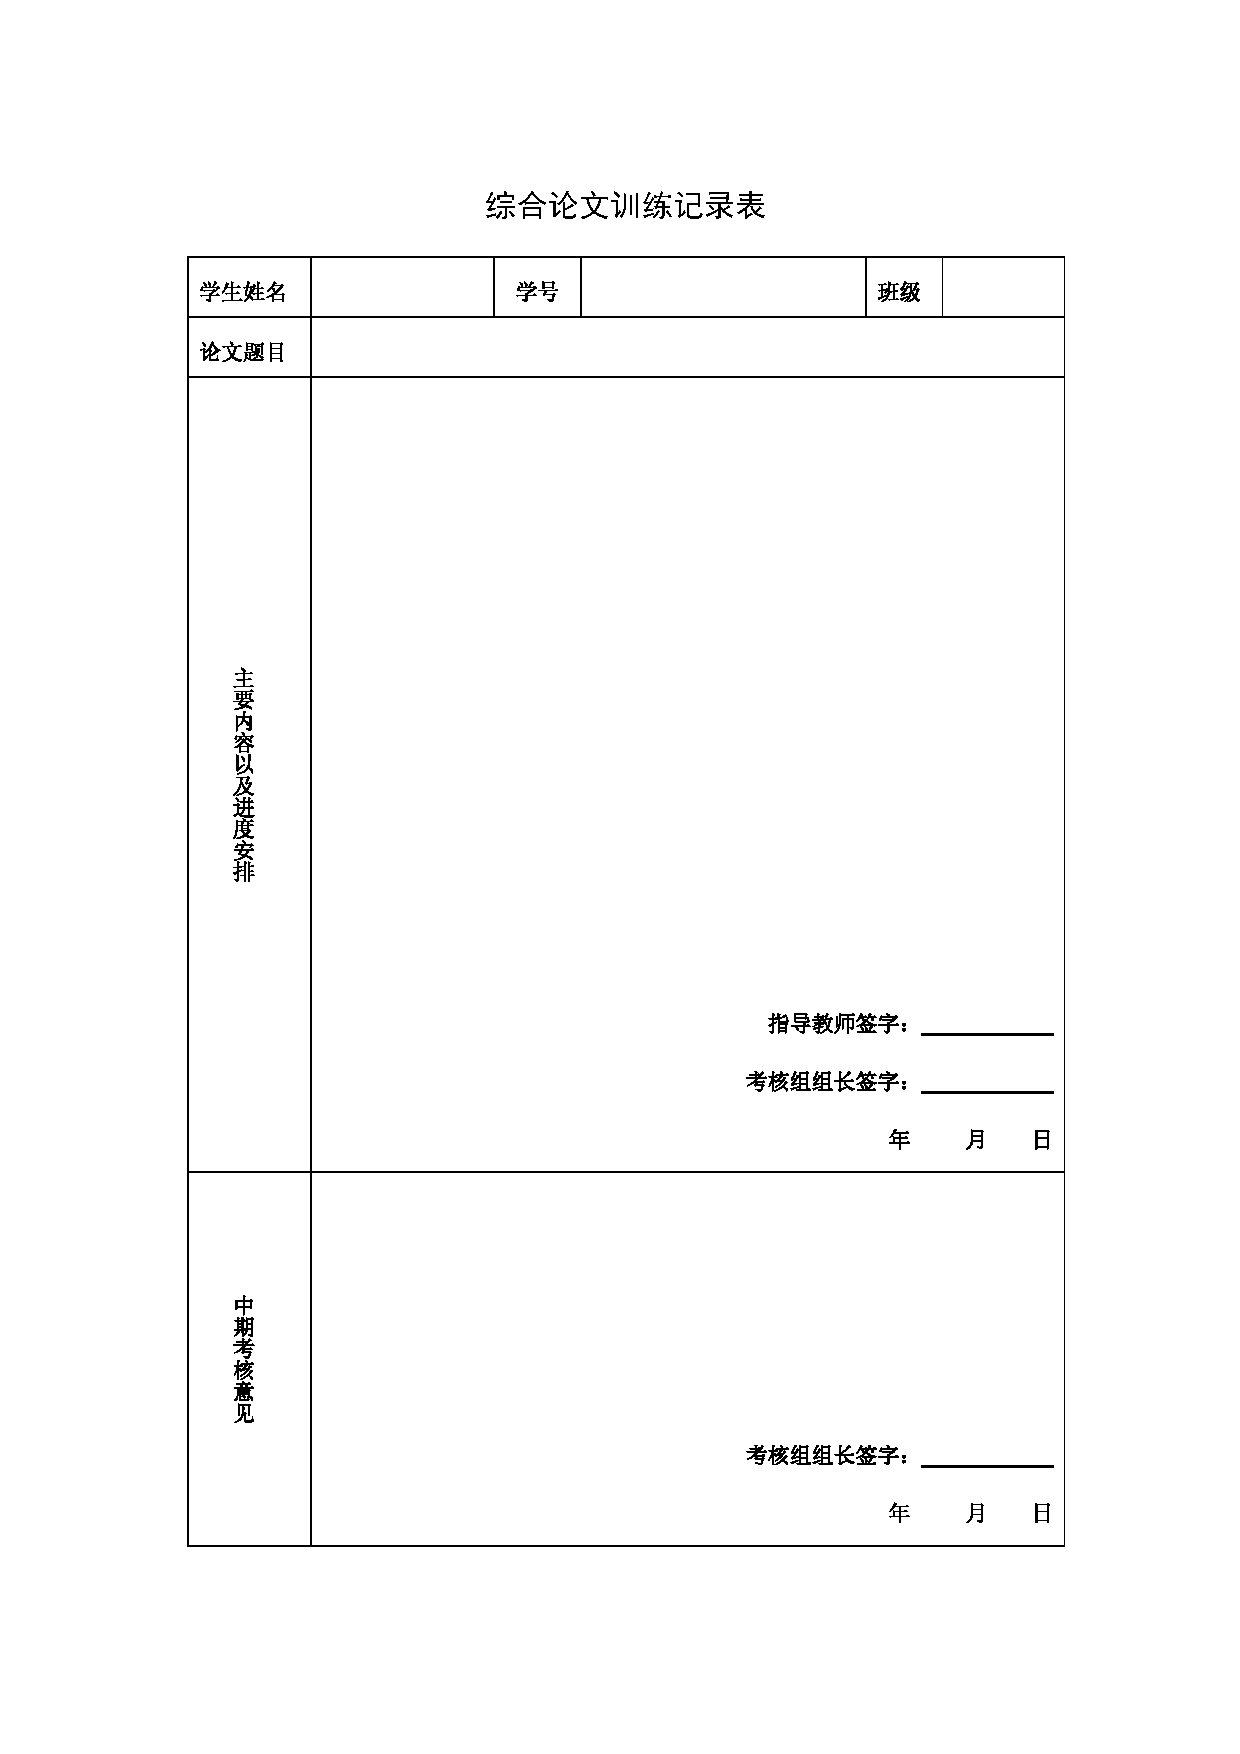
\includepdf[pages=-]{scan-record.pdf}
\end{document}
